\documentclass[english]{amu_these}

\begin{document}


	\chead{}
\pdfbookmark[0]{Page de titre}{titre}
\thispagestyle{empty}
\newgeometry{margin=2em}
% \newgeometry{left=3em,right=2em,top=2em,bottom=2em} %% marge pour la reliure en cas d'exemplaire imprimé

\begin{center}
	\begin{minipage}[c]{.5\linewidth}
		\raggedright\includegraphics[height=7em]{logo_amu_excellence}
	\end{minipage}\hfill
	\begin{minipage}[c]{.5\linewidth}
		%\raggedleft\includegraphics[height=7em]{example-image-b} %% logo cotutelle
	\end{minipage}\hfill
\end{center}

\vspace{1em}

\begin{center}
	\begin{minipage}[c]{.63\linewidth}
		\dhorline{\textwidth}{4pt}
	\end{minipage}\hfill
	\begin{minipage}[c]{.35\linewidth}
		\raggedleft\titl{NNT/NL : 2020AIXM0001/001ED000}
		% renseigner votre numéro national de thèse (NNT) et le numéro local (NL)
		% ils sont indiqués sur la page d'informations administratives de votre espace de dépôt dans le guichet de dépôt légal des thèses AMU lorque votre date de soutenance est renseignée par votre service de scolarité
		% https://depot-theses.univ-amu.fr/
	\end{minipage}\hfill
\end{center}

%\vspace{1em}

\doublespacing
\begin{flushleft}
    \titb{\HUGE\textcolor{cyanamu}{THÈSE DE DOCTORAT}}\\
	\titl{\Large Soutenue à Aix-Marseille Université}\\
	%\titl{\Large dans le cadre d'une cotutelle avec }\\
	\titl{\Large le 27 Octobre 2023}\\
\end{flushleft}
\vspace{2em}
\begin{center}
	\titsb{\Huge Pierre LECHIFFLART}\\
    \vspace{1em}
	\titm{\LARGE Exciton-phonon coupling and phonon-assisted luminescence in hexagonal Boron Nitride nanostructures}\\
\end{center}
\singlespacing

\vspace{4em}

\begin{center}
	\begin{minipage}[t]{.45\linewidth}
    	    \vspace{.5em}
        	\titb{Discipline}
        	
        	\titl{Physique et Sciences de la Matière}
        	
    	    \vspace{1em}
        	\titb{Spécialité}
        	
        	\titl{Matière Condensée et Nanosciences}
        	
    	    \vspace{2em}
        	\titb{École doctorale}
        	
        	\titl{352 PHYSIQUE ET SCIENCES DE LA MATIERE}
        	
    	    \vspace{1em}
        	\titb{Laboratoire/Partenaires de recherche}
        	
        	\titl{CINaM - Centre Interdisciplinaire de Nanosciences de Marseille / UMR 7325
        	}
	\end{minipage}\hfill
	\begin{minipage}[t]{.03\linewidth}
	    \dvertline{4pt}{-16em}
	\end{minipage}\hfill
	\begin{minipage}[t]{.52\linewidth}
	    \vspace{.5em}
    	\titb{\small Composition du jury}

	    \vspace{1em}
    	\titel{
        \begin{tabular}{p{12em} p{9.5em}}
        	Olivia PULCI & Rapporteuse \\
        	Université de Rome Tor Vergata \\
        	\\
        	Sylvain LATTIL & Rapporteur \\
        	CEA Saclay \\
            \\
            Valerio OLEVANO & Examinateur \\
        	Institut Néel, Grenoble \\
            \\
        	Aurélien MANCHON & Président du jury \\
        	Aix-Marseille Université, CINaM \\
            \\
        	Claudio ATTACCALITE & Directeur de thèse \\
        	CNRS-CINaM, Marseille \\
        \end{tabular}
        }
	\end{minipage}\hfill
\end{center}       

\vspace{2em}

\begin{center} %% logos partenaires
	\begin{minipage}[c]{.25\linewidth}
		\centering
\includegraphics[height=5em]{logo/logo-cinam} 
	\end{minipage}\hfill
	% \begin{minipage}[c]{.25\linewidth}
	% 	\centering\includegraphics[height=5em]{example-image-b}
	% \end{minipage}\hfill
\end{center}

\restoregeometry				%% page de titre

	\newpage 
\
\newpage
\chapter*{Affidavit}					
\addcontentsline{toc}{chapter}{Affidavit}
\thispagestyle{empty}
\iffalse % Déclaration sur l'honneur pour une thèse en français (inverser les \if pour une thèse en anglais)
    Je soussigné, [Prénom Nom], %% Prénom et Nom de l'auteur %%
    déclare par la présente que le travail présenté dans ce manuscrit est mon propre travail, réalisé sous la direction scientifique de [Prénom Nom], % Prénom et Nom du directeur de thèse et s’il y a lieu du co-directeur de thèse
    dans le respect des principes d’honnêteté, d'intégrité et de responsabilité inhérents à la mission de recherche. Les travaux de recherche et la rédaction de ce manuscrit ont été réalisés dans le respect à la fois de la charte nationale de déontologie des métiers de la recherche et de la charte d’Aix-Marseille Université relative à la lutte contre le plagiat.
    
    Ce travail n'a pas été précédemment soumis en France ou à l'étranger dans une version identique ou similaire à un organisme examinateur.\\
    
    Fait à [ville] le [date]
    
    \begin{flushright}\includegraphics[width=120px,height=40px]{example-image-a}\end{flushright}% signature
\fi

\iftrue % Affidavit of Honour for english thesis (invert the \if for an English thesis)
    I, undersigned, Pierre Lechifflart, %% First Name and Surname of the PhD student
    hereby declare that the work presented in this manuscript is my own work, carried out under the scientific direction of Dr. Claudio Attaccalite, %% First Name and Surname of the thesis director and if applicable of the co-thesis director
    in accordance with the principles of honesty, integrity and responsibility inherent to the research mission. The research work and the writing of this manuscript have been carried out in compliance with both the french national charter for Research Integrity and the Aix-Marseille University charter on the fight against plagiarism.
    
    This work has not been submitted previously either in this country or in another country in the same or in a similar version to any other examination body.\\
    
    Marseille, 28 August 2023
    
    \begin{flushright}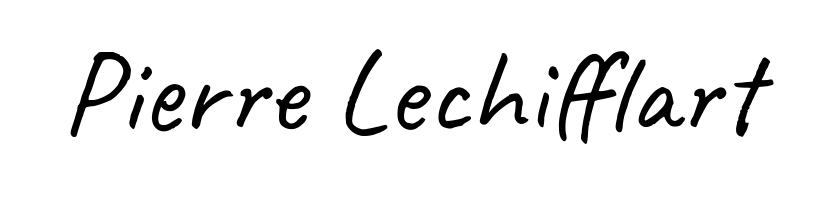
\includegraphics[width=60px,height=23px]{signaturePL.png} \ 
\includegraphics[width=46px,height=59px]{signature_pierre.png}\end{flushright} % signature
\fi

~\vfill
\begin{center}
	\begin{minipage}[c]{0.25\linewidth}
		\includegraphics[height=35px]{by-nc-nd-eu}
	\end{minipage}\hfill
\end{center}

Cette \oe{}uvre est mise à disposition selon les termes de la \href{https://creativecommons.org/licenses/by-nc-nd/4.0/deed.fr}{Licence Creative Commons Attribution - Pas d’Utilisation Commerciale - Pas de Modification 4.0 International}. % consultez les conditions de la licence cc by-nc-nd, vous pouvez appliquer une licence moins restrictive, cc by-nc-sa par exemple
				%% affidavit et licence

	\newpage
\chapter*{Liste de publications et participation aux conférences}
\addcontentsline{toc}{chapter}{Liste de publications et participation aux conférences}
\subsection*{Liste des publications réalisées dans le cadre du projet de thèse:}
\begin{enumerate}
\item \underline{Pierre Lechifflart}, Fulvio Paleari and Claudio Attaccalite. “Excitons under strain: light absorption and emission in strained
hexagonal boron nitride”. In: SciPost Physics 12 (May 2022), p. 145.
\item \underline{Pierre Lechifflart}, Fulvio Paleari, Davide Sangalli and Claudio Attaccalite. “First-principles study of luminescence in hexagonal boron
nitride single layer: Exciton-phonon coupling and the role of substrate”. In: Physical Review Materials 7.2 (Feb. 2023).
\item Michele Re Fiorentin, \underline{Pierre Lechifflart} and Fulvio Paleari, "Electronic structure and luminescence of Bernal Boron Nitride", \textit{en péparation}.
\end{enumerate}


\subsection*{Participation aux conférences et écoles d’été au cours de la période de thèse:}
\begin{enumerate}
\item Virtual school on electronic excitations in solids and nanostructures using the Yambo code, Avril 2021, en ligne
\item 17th ETSF Young Researchers Meeting, Septembre 2021, Cagliari
\item 12th Meeting on NanoScience Advances, Septembre 2021, Porquerolles
\item School : ab initio Many-body methods and simulations with the yambo code, Avril 2022, Trieste  
\item 25th ETSF Workshop, Juin 2022, Leuven
\item 18th ETSF Young Researchers Meeting, Septembre 2022, Marseille
\item Green's function methods : the next generation Workshop, Novembre 2022, Toulouse
\item GDR HOWDI annual meeting, Mai 2023, Porquerolles
\item International BN Workshop, Mai 2023, Montpellier
\end{enumerate}			%% liste de publications et participation aux conférences

	\chapter*{Résumé}
\addcontentsline{toc}{chapter}{Résumé}

%

%

\selectlanguage{french}
La présente thèse de doctorat explore l'interaction complexe entre les excitons et les phonons dans les nanostructures de nitrure de bore hexagonal (hBN) à l'aide de méthodes de calcul avancées. La thèse commence par une introduction au hBN, mettant en lumière ses propriétés uniques et son importance dans la physique de la matière condensée. 

Le chapitre 2 donne un aperçu complet du cadre théorique de pointe utilisé tout au long de la recherche, englobant la théorie de la fonctionnelle de la densité (DFT), la théorie des perturbations de la fonctionnelle de la densité (DFPT) pour les propriétés des phonons, et la théorie des perturbations à N-corps (MBPT) à travers l'approximation GW et l'équation de Bethe-Salpeter pour prendre en compte les effets collectifs électroniques et excitoniques.

Dans le chapitre 3, l'accent est mis sur le hBN massif soumis à une déformation uniaxiale, où le couplage exciton-phonon est étudié à l'aide d'une méthode de dérivation par différences finies. Cette approche reproduit approximativement les changements d'intensité de la luminescence observés lorsqu'une contrainte est appliquée au cristal. Les résultats de ce chapitre donnent des indications précieuses sur les propriétés électroniques, phononiques et excitoniques, ainsi que sur les interactions exciton-phonon dans les systèmes hBN massifs soumis à une déformation uniaxiale.

Le chapitre 4 se penche sur l'étude du hBN monocouche, en utilisant une méthode ab initio fondée sur une dérivation théorique rigoureuse des éléments de matrice du couplage exciton-phonon. En incorporant les pics directs et indirects dans les spectres de luminescence, cette méthode donne des intensités relatives détaillées, permettant une interprétation précise des mesures expérimentales publiées par différents groupes de recherche. Notamment, cette étude élimine la possibilité d'observer des répliques de phonons dans les spectres du hBN monocouche, apportant une nouvelle clarté à des interprétations auparavant ambiguës.

En outre, la thèse présente des résultats préliminaires pour le BN Bernal, un polytype de hBN avec un empilement de couches différent, présentant des gaps d'énergie directs et indirects très proches les uns des autres. Ce matériau intrigant a le potentiel d'afficher simultanément des pics directs et indirects dans les spectres de luminescence. Dans le cadre des recherches en cours qui incluent une étude numérique poussée, ce chapitre ouvre la voie à une compréhension plus approfondie des interactions exciton-phonon dans la phase Bernal du BN.

Dans l'ensemble, cette thèse de doctorat contribue de manière significative au domaine de la physique computationnelle de la matière condensée en clarifiant les phénomènes complexes de couplage exciton-phonon dans diverses nanostructures hBN. Les connaissances acquises grâce à cette étude peuvent faire progresser la compréhension et la conception de nouveaux dispositifs optoélectroniques basés sur des matériaux hBN.

\vspace{0.5cm}
Mots-clés: luminescence, phonons, excitons, couplage exciton-phonon					%% résumé

	\chapter*{Abstract}
\addcontentsline{toc}{chapter}{Abstract}
\selectlanguage{english}

The present PhD thesis explores the intricate interplay between excitons and phonons in hexagonal Boron Nitride (hBN) nanostructures through advanced computational methods. The thesis commences with an introduction to hBN, shedding light on its unique properties and relevance in condensed matter physics. 

Chapter 2 provides a comprehensive overview of the state-of-the-art theoretical framework employed throughout the research, encompassing Density Functional Theory (DFT), Density Functional Perturbation Theory (DFPT) for phonon properties, and Many-Body Perturbation Theory (MBPT) through the GW approximation and the Bethe-Salpeter equation to account for collective electronic and excitonic effects.

In Chapter 3, the focus lies on uniaxially strained bulk hBN, where the exciton-phonon coupling is studied using a finite-difference derivative method. This approach approximately reproduces the changes in luminescence intensity observed when strain is applied to the crystal. The outcomes of this chapter offer valuable insights into the electronic, phononic and excitonic properties, as well as exciton-phonon interactions in bulk hBN systems under uniaxial strain.

Chapter 4 delves into the investigation of monolayer hBN, employing an ab initio method grounded on a rigorous theoretical derivation of the exciton-phonon coupling matrix elements. By incorporating both direct and indirect peaks in the luminescence spectra, this method yields detailed relative intensities, enabling an accurate interpretation of experimental measurements published by different research groups. Notably, this study eliminates the possibility of observing phonon replicas in the spectra of monolayer hBN, providing new clarity to previously ambiguous interpretations.

Furthermore, the thesis offers preliminary results for Bernal BN, a polytype of hBN with a different layer stacking, featuring closely situated direct and indirect energy gaps. This intriguing material holds potential for displaying simultaneously both direct and indirect peaks in luminescence spectra. As part of ongoing research that includes deep numerical studies, this chapter paves the way for a deeper understanding of exciton-phonon interactions in Bernal BN structures.

Overall, this PhD thesis contributes significantly to the field of computational condensed matter physics by unraveling the complex exciton-phonon coupling phenomena in various hBN nanostructures. The insights gained from this study have the potential to advance the understanding and design of novel optoelectronic devices based on hBN materials.

\vspace{0.5cm}
Keywords: luminescence, excitons, phonons, exciton-phonon coupling

				%% abstract

	\chapter*{Acknowledgments / Remerciements}
\addcontentsline{toc}{chapter}{Acknowledgments / Remerciements}

First I would like to thank the board of Doctoral School 352 that granted me this PhD funding, Andrea Marini for hosting me one week in Rome, funded by the Cost Action TUMIEE, Daniele Varsano and HPC Europa3 for allowing me a 2-month visit in Modena.

I would like to thank my supervisor Claudio for his constant support, his availability, for giving me the freedom to study the things I wanted and for his wise decisions that helped me to become a scientist. Un ringraziamento speciale per il tempo che hai dedicato alla revisione di questo manoscritto.


I would like to thank Khaoula Boukari and Andres Saul for the management and maintenance of the computer cluster \textit{Rosa} which was an undeniable advantage for this PhD work.

I thank the TSN department as a whole for scientific discussions and at large, everyone who I discussed about science with and who sated my hunger for understanding, Elena Cannuccia, Adrien Rousseau, Thibaut Sohier, Pedro Melo, Martino Silvetti, Matteo Zanfrognini, Riccardo Reho.

I thank the people I met in CINaM and who became my friends : Anna, Petr, Clémence, Céline, Alex, Julien, Diego, Ilan, Rajarshi, Guillem, Djouher, Mathilde, Kostis, Tarik, Gaëlle, Giorgia, Luigi,  Mohit, Vyshnav. You contributed to brighten the sometimes gloomy days. 

I thank Vitaly, Laura, Miguel and Kalyani for their help in the organization of YRM 2022 which was quite an experience, Véronique, Régine, Lydia, Cindy, Sabina for the precious administrative help, and Christophe for the budgetary rescue.

I thank Marine Baujon for helping me manage things that felt bigger than me at times.

I thank everyone for good times in Marseille and elsewhere Sam, Yann, Jonathan, Pavlo, Vasile, Thaïs, Simon, Inès.

Merci à mes proches qui donnent un sens à tout ceci. Jules, Pieric, Valentin, Yann, merci de votre soutien indéfectible, vous êtes des amis formidables.

Un simple merci ne suffirait pas pour exprimer ma gratitude envers mes parents et ma famille. Merci Maman et Papa pour m'avoir toujours soutenu et exprimé votre fierté. Merci Baptiste et Maxime d'être des frères admirables. Merci Côme et Thaïs de bien vouloir jouer avec moi.				%% remerciements

    \microtypesetup{protrusion=false}	%% désactive la protrusion (TOC LOFT GLS)
	\tableofcontents					%% TOC
	\listoffigures						%% LOF
	\listoftables						%% LOT
	\printglossary[						%% acronymes
		type=\acronymtype,
		title={List of acronyms},
		toctitle={List of acronyms}
		]
	\printglossary[						%% glossaire
		title={Glossary},
		toctitle={Glossary}
		]
	% \printglossary[						%% nomenclature
	% 	type=notation,
	% 	title={Nomenclature},
	% 	toctitle={Nomenclature}
	% 	]
    \microtypesetup{protrusion=true}	%% rétabli la protrusion

	\ohead{\leftmark\Ifstr{\rightmark}{\leftmark}{}{ -- \rightmark}}	%% place le chapitre et la partie en en-tête

	\chapter*{Introduction}
\addcontentsline{toc}{chapter}{Introduction}
Generalities about hBN \\
We could compute phonon-assisted absorption but the phonon satellites are very small wrt to the main peaks so when they overlap, they are not visible.\\
Theory of phonon-assisted optics : it exists. For instance, Williams-Lax theory that treats lattice-dependent band features and phonon-assisted transitions 
There is also Hallen-Bardeen-Blatt and Heine-Cardona but I don't know too much about them.
Besides, some models of exciton-phonon coupling exists also, some specifically for luminescence, but they are computationally expensive for real materials.
==> there is a need for exciton-phonon coupling and phonon-assisted optics from first principles. In chapters 2 and 3, two different approaches are presented in section \textcolor{red}{ref to sections}. The first one consists in calculating the response function correction due to exciton-phonon coupling from finite differences, by displacing atoms in supercells. The second one is a more general approach based on \acrshort{MBPT}, in which a dynamical correction induced by electron-phonon coupling is added as a perturbation to the Bethe-Salpeter kernel. Thanks to this \textit{ab initio} framework, the scattering of every exciton with every phonon mode can be computed, over the whole Brillouin Zone. These calculations are done in the unit cell.
Both approaches allow to compute the exciton-phonon coupling. Then, the absorption can be obtained after post-processing of a standard \acrshort{BSE} calculation. To obtain the luminescence spectra, we use the van Roosbroeck -- Shockley relation for both cases.
Exciton-phonon in hBN are not only possible, but likely due to strong electron-phonon coupling. Verified experimentally by the External Quantum Efficiency comparable to direct gap materials.
%
%
%
ETSF webinar of Fulvio
indirect bandgap only; we can write the response function with derivatives of the response function because we consider only phonon-assisted transitions; need supercells
converge the displacement so that it is the smallest possible
PLE (propto absorption) or absorption and PL are not symmetric, as expected for direct gaps
the minimum exciton at T is the degenerate dark state at Gamma which splits
for absorption, the bright exciton overlaps with the phonon replicas and it is so bright that we don't see them 

	\chapter{Hexagonal Boron Nitride under strain}
\chaptertoc{}

\textit{This chapter is partly based on our publication Ref. \cite{lechifflart2022excitons}. Some of the text and figures contained in this Chapter are adapted from this reference.}

%
\section{Introduction and experimental motivations}
\textcolor{red}{Do you think I should put this in the Introduction chapter ?}
Strain is a powerful tool to engineer electronic and optical properties of materials. It is possible to modify the electronic dispersion of strained crystals, in particular to modify the conduction band minima and the valence band maxima, even leading to a direct to indirect bandgap transition, as it was shown for Germanium \cite{hoshina2009first,cheng2010strain} and more recently for transition metal dichalcogenides.\cite{desai2014strain,choudhary2020shear,frisenda2017biaxial} Regarding hBN, the effect of strain on vibrational properties was investigated experimentally in exfoliated hBN with various thicknesses,\cite{androulidakis2018strained} while theoretically biaxial tensile strain was considered for the mono- and bilayer h-BN \cite{yang2013distorted,fujimoto2016band} as well as its role on hexagonal boron nitride quantum emitters.\cite{tabesh2021strain} But little is known about the effect of strain on the optical properties of bulk h-BN, which are the simplest mean to characterize this material. \\
A recent experiment showed a remarkable modification of the cathodoluminescence spectrum of hBN under strain. \cite{schue2017proprietes} In this experiment Léonard Schué, from the group of Julien Barjon, suspended a nanosheet of hexagonal Boron Nitride over a trench carved out from an SiO$_2$ substrate. The nanosheet is about 100 nm thick and curves under the effect of gravity, as illustrated in Fig. \ref{fig:exp_strain}(a), and was imaged by \acrfull{AFM} (Fig. \ref{fig:exp_strain}(b)).
\begin{figure}[tbp]
	\vspace{0.2cm}
	\setcapindent{2em}
	\centering
	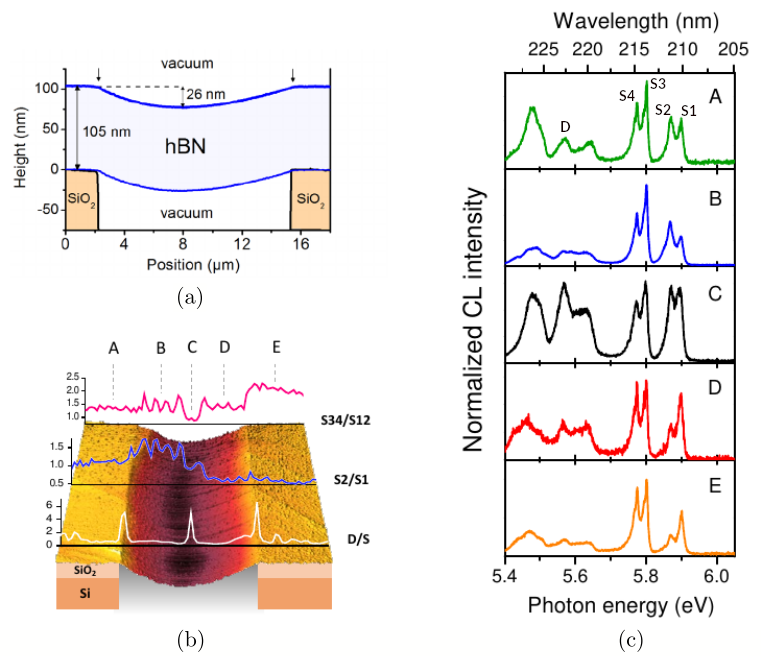
\includegraphics[width=0.7\textwidth]{exp_strain.png}
	\caption{(a) Sketch of the deposited hBN nanosheet on the trench. (b) AFM profile and relative intensity ratios of different emission peaks with respect to spatial region. (c) Cathodoluminescence intensity measured on different regions of the sample. Courtesy of Léonard Schué and Julien Barjon}
	\label{fig:exp_strain}
\end{figure}
When measuring the cathodoluminescence spectra at different positions on the sample, one can see that the intensity ratios between different peaks are varying. Their interpretation is that the deformation of the sample induces uniaxial (compressive) strain, perpendicular to the trench. This strain could have an effect on the recombination process of excitons or their scattering with phonons, leading to a change in the luminescence intensity. The measure an intensity ratio between the S1/2 and the S3/4 peaks coming from $\approx 4$ at equilibrium to almost 1 at the bottom of the trench. We try to simulate this phenomenon and use a method to reproduce the phonon-assisted luminescence from first-principles.


%
\section{Structure and phonons}
In order to simulate the hBN sample in suspension, we consider an infinite bulk crystal under uniaxial strain. In the experiment, the beam of electron penetrates only on the upper part of the nanosheet, where the strain is compressive. However for the first steps of the computational workflow, we study a range of strain including both stretching and compression around the equilibrium structure.
First, we obtain the strained structure by taking an orthorombic cell of the pristine crystal, larger than the hexagonal unit cell. Because it has three orthogonal lattice vectors, the orthorombic cell is more suited for the application of a uniaxial strain. To do so, we simply alter the length of one cell vector, up to an arbitrary length corresponding to a value of strain. We studied different strain values, in an interval going from a $+2.5\%$ to a $-2.5\%$ variation of the equilibrium length. In this work we applied strained in the armchair direction, the one parallel to the B-N bond. 
\begin{figure}[tbp]
	\vspace{0.5cm}
	\setcapindent{2em}
	\centering
	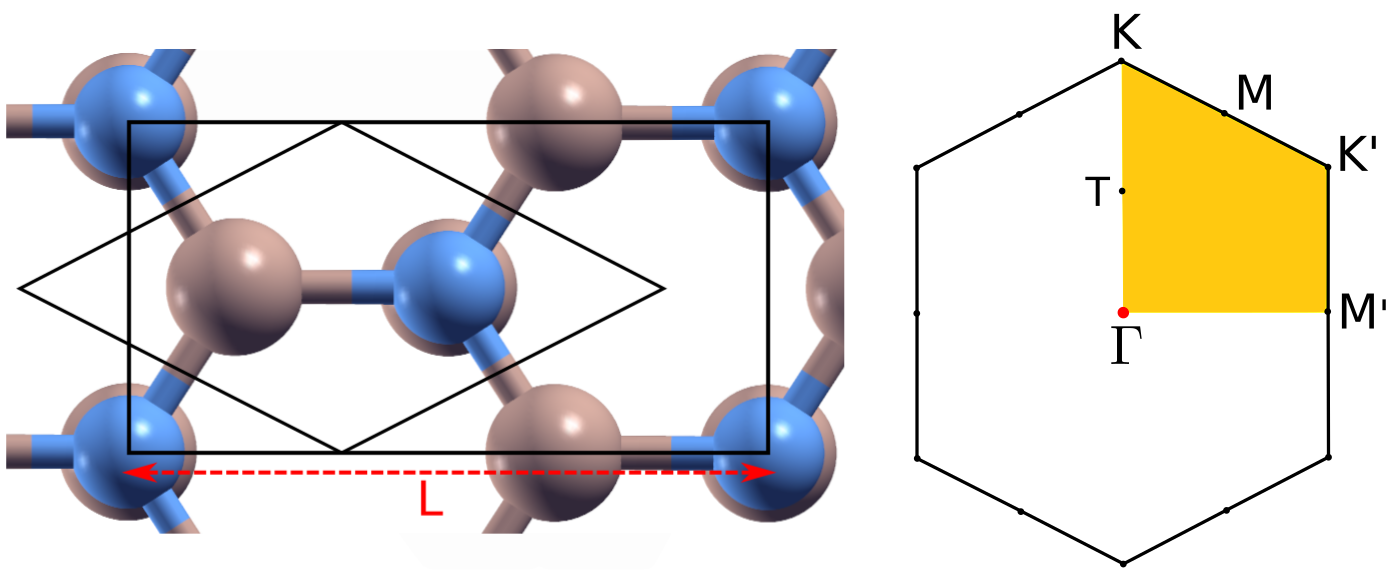
\includegraphics[width=0.8\textwidth]{AppB_structure_BZ.png}
	\caption{Left : visualization of the strained crystal and the orthorombic and pseudo-hexagonal unit cells. Right : corresponding strained Brillouin Zone. The dotted line is the shape of the equilibrium BZ. The yellow zone is the area enclosed by the high-symmetry points we used to plot dispersions.}
	\label{fig:strain_BZ}
\end{figure}
After setting the length of the cell to the desired length corresponding to a strain value, we let the atom positions and the other two cell vectors relax, using a damped molecular dynamics algorithm where the forces acting on the atoms are computed in \acrshort{DFT} using the Hellmann--Feynman theorem. This procedure in implemented in the \qe ~suite.\cite{giannozzi2009quantum,giannozzi2017advanced} More computational details can be found in Appendix \ref{app:comp_par_strain}. We found that once the two cell vectors orthogonal to the strained one are relaxed, their length vary linearly with the strain.\\
Once we have the relaxed strained orthorombic cells, we want to construct a pseudo-hexagonal unit cell containing only four atoms. This way, we can compare the structures obtained for different strain values with the equilibrium structure in a consistent way and proceed with the calculation of electronic and optical properties. To construct the pseudo-hexagonal cells from the strained orthorombic ones, we followed the procedure described in Appendix \ref{app:ortho2hex}. We computed the phonon-related properties using \acrshort{DFPT} in the four-atom strained cells. In the strained crystal, whatever the value of strain, the 120\textdegree~ rotational symmetry is broken and this makes the \MM~and \KK~points in the \acrshort{BZ} inequivalent to the \MM' and \KK' points. The path between high-symmetry points containing all four of these points is drawn in yellow in Fig. \ref{fig:strain_BZ}.
The resulting phonon dispersions are shown in Fig. \ref{fig:strain_phonons}, for three strain values : a $+2.5\%$ stretch, a $-2.5\%$ compression and the equilibrium one.
\begin{figure}[tbp]
	\vspace{0.5cm}
	\setcapindent{2em}
	\centering
	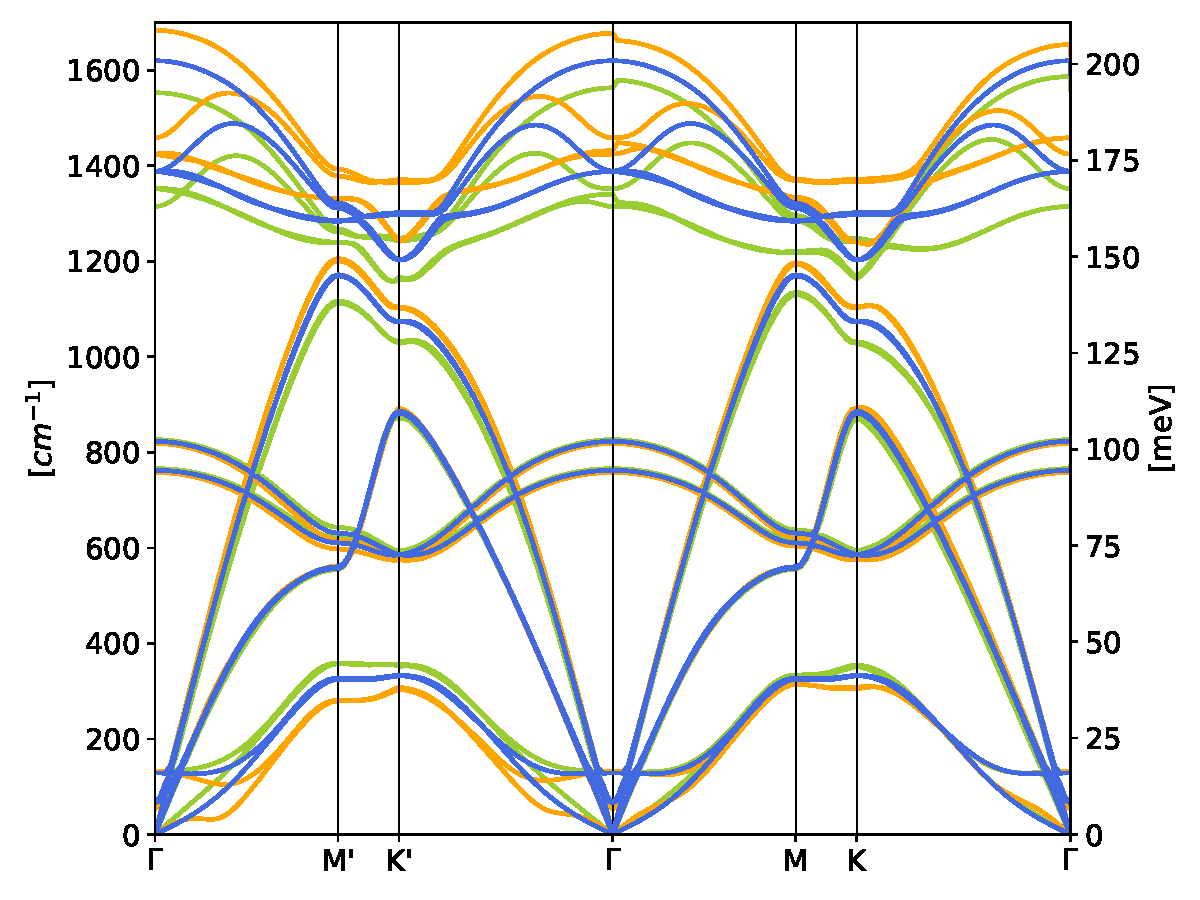
\includegraphics[width=0.8\textwidth]{strain_ph.pdf}
	\caption{Phonon dispersion versus uniaxial strain. Blue lines are at equilibrium, green lines at 2.5\% stretch and orange lines at 2.5\% compression.}
	\label{fig:strain_phonons}
\end{figure}
For the unstrained dispersion we can notice the splitting of the highest branch at $\Gamma$ with the two branches below. This is the LO-TO splitting mentionned in Sec. \ref{sec:DFPT}.

We found that the optical modes (the branches with the highest energies) are the most affected by strain. With compressive strain, their frequencies are increased at all $\qq$ points and they are decreased for tensile strain. We also observe the splitting of the E$_{2g}$ modes, whose frequencies are degenerate at $\Gamma$ just below 175 meV or 1400 cm$^{-1}$ for the unstrained structure. They split as soon as a strain is applied. This is in agreement with Raman measurements and previous calculations.\cite{blundo2022vibrational,androulidakis2018strained} It is also interesting to notice that depending on the direction along which the $\Gamma$ point is approached, the splitting of the two E$_{2g}$ modes has different magnitudes. 

On the mid-energy range of the dispersion, the LA, TA and TO modes are not very affected by strain. This will be important in the discussion about luminescence in the following.

On the lower frequency end, the acoustic modes are affected in an opposite way. Under compression, their frequencies are decreased and increased under stretch. The orange curve shows a softening of the lowest branch close to $\Gamma$. We noticed that increasing the value of compressive strain leads to giving imaginary frequencies. This happens when the geometry is unstable. Then the second derivative in Eq. \eqref{eq:IFC_matrix} is negative and the eigenvalues $\omega^2$ in Eq. \eqref{eq:ph_evprob} are negative. We did not investigate this instability caused by compression, since the range of strain we are interested in is not above $+2.5\%$ of strain. Nonetheless, the phonon dispersions show that our systems are stable in the range of strain considered.

%
\section{Electronic structure}
After computing the Kohn-Sham eigenvalues in \acrshort{DFT}, we performed a one-shot G$_0$W$_0$ calculation to compute the quasiparticle corrections using the \yambo code. We found that these corrections are a rigid shift in energy of the KS eigenvalues over the whole \acrshort{BZ}. 
\begin{figure}[tbp]
	\vspace{0.5cm}
	\setcapindent{2em}
	\centering
	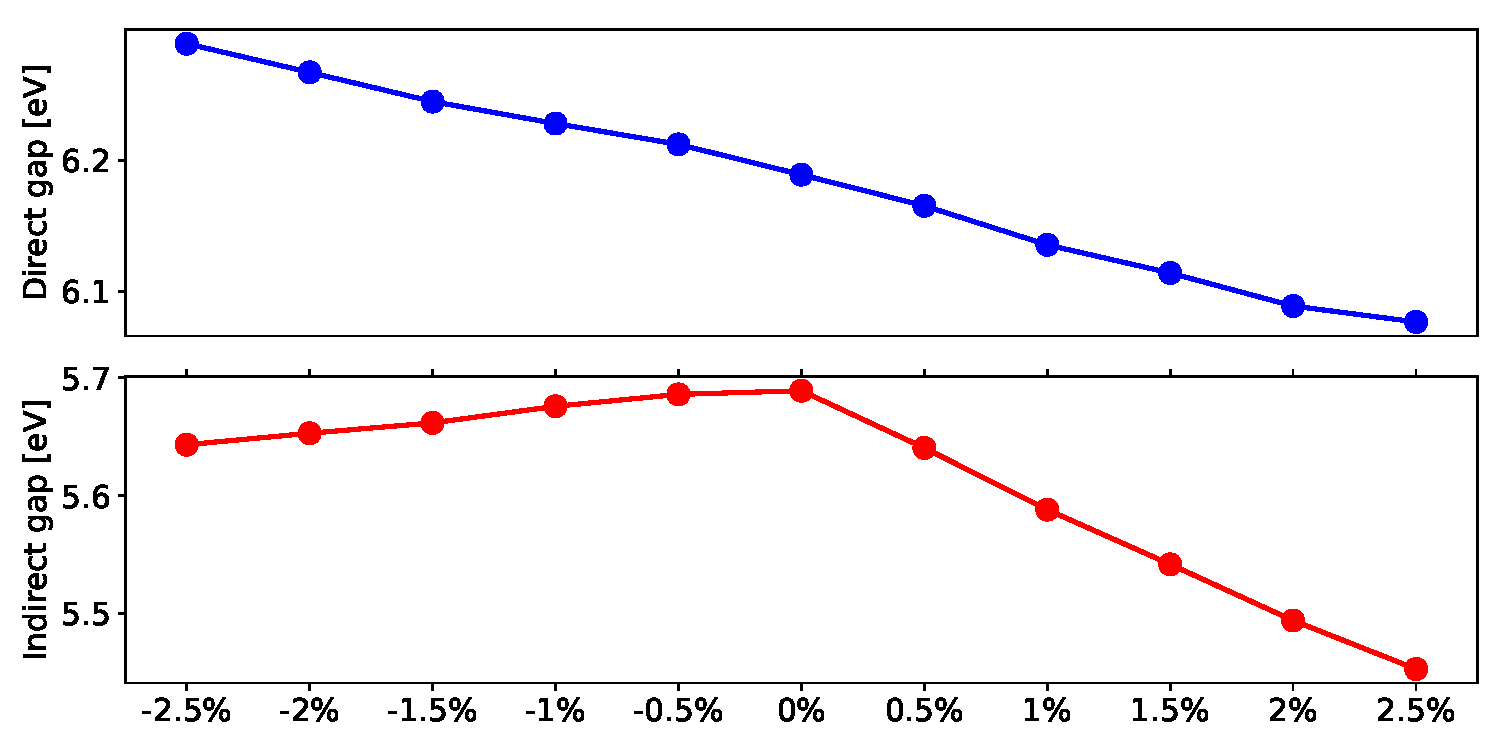
\includegraphics[width=0.8\textwidth]{strain_gw_gaps.pdf}
	\caption{Quasiparticle corrections to the direct and indirect bandgaps at the G$_0$W$_0$ level with respect to strain.}
	\label{fig:strain_gw_gaps}
\end{figure}
In Fig. \ref{fig:strain_gw_gaps} we report the variation of the direct gap (at \MM) and of the indirect gap (between \KK~and \MM) with respect to strain. The direct gap has decreases linearly with increasing relative values of strain, while the indirect gap is maximal for the unstrained system and decreases both for compression and stretch.

The electronic dispersions along the path showed above are plotted in Fig. \ref{fig:strain_eldisp} for the two maximally strained systems and for the unstrained one. 
\begin{figure}[tbp]
	\vspace{0.5cm}
	\setcapindent{2em}
	\centering
	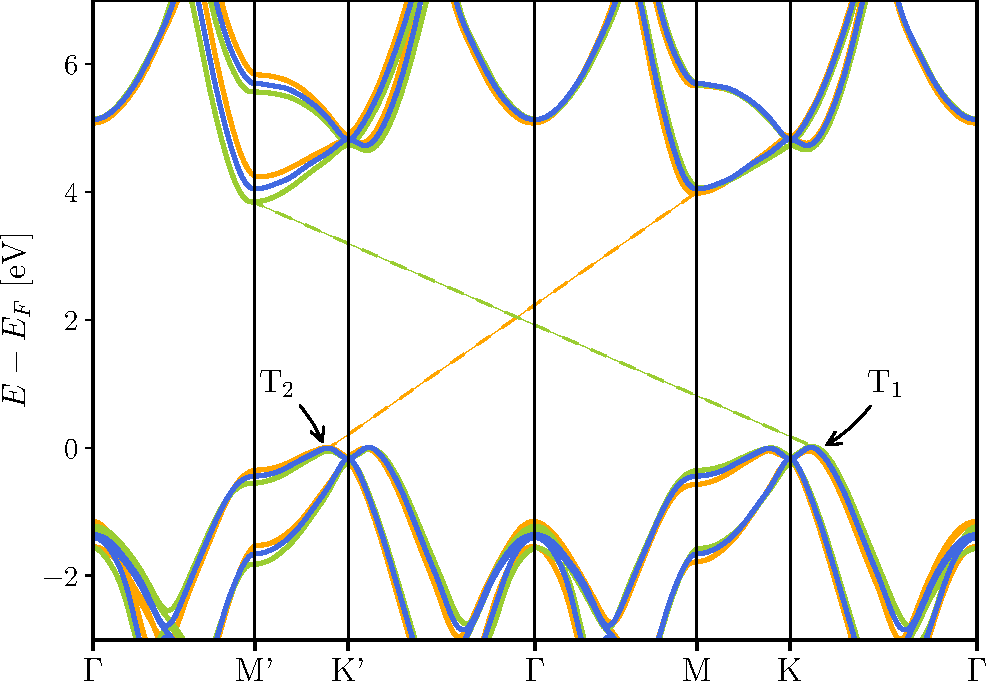
\includegraphics[width=0.6\textwidth]{strain_bands_qgaps.pdf}
	\caption{Details of the electronic band structure under the maximum
	stretch and compression considered in the manuscript. Blue lines are at equilibrium, green lines at +2.5\% stretch and orange lines at -2.5\% compression. We report also the location of the new indirect gaps in the two cases. Notice that at equilibrium all indirect transitions between the different \KK~ and \MM~ points are equivalent.}
	\label{fig:strain_eldisp}
\end{figure}
At equilibrium, the direct gap is located between states with a momentum close to \KK. The indirect gap is between a point close to \KK~for the valence band and the \MM~point for the conduction band. As discussed above, strain breaks one of the symmetries of the crystal and this effect is visible on the dispersions at high-symmetry points. Under compression, the conduction band is shifted down at \MM~while it is increased at \MM'. This trend is reversed under stretch. Hence, the conduction band minimum is at \MM~for the compressed crystal and at \MM' for the stretched crystal. 
These variations can be explained in term of the variation of the orbital properties. 
\begin{wrapfigure}{r}{0.41\textwidth}
	\vspace{-16pt}
	\setcapindent{1em}
	\centering
	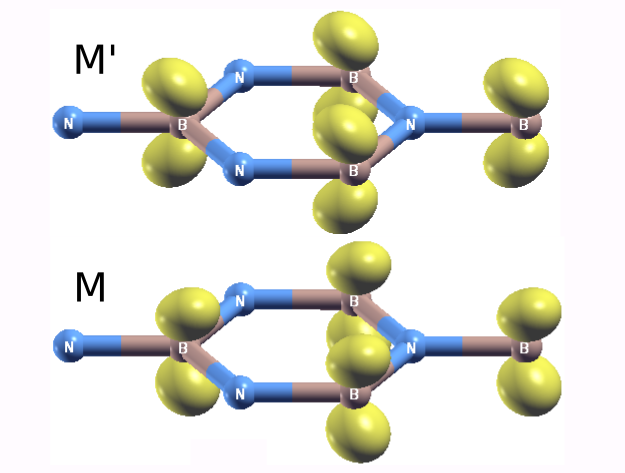
\includegraphics[width=0.4\textwidth]{M_and_M_prime.png}
	\caption{$\pi^*$ atomic-like orbitals of the conduction band minima on one of the layers for a compression of 0.5\%. At \MM', the components of the wavefunctions are oriented along the compressed B-N bond. At \MM, they are oriented along one of the other bonds.}%\textcolor{red}{Rajoute des flèches pour montrer le strain.}}
	\label{fig:WF_strain}
\end{wrapfigure}
The $\pi^*$ atomic-like orbitals at \MM~and \MM' have a different shape, as illustrated in Fig. \ref{fig:WF_strain} for a compression of 0.5\%. While they are degenerated in energy for the unstrained crystal, this degeneracy is lifted due to the symmetry breaking. The state with orbital components along the strained bond is the one whose energy changes with strain at \MM'. These orbitals are dependent on the interlayer interactions, which in turns depends on the interlayer distance. This distance varies linearly with the strain applied to the system in our relaxation process. This explains the splitting of the bands induced by strain at the \MM' point.

The valence states around \KK~and \KK' are only slightly changed in energy. This can be explained because the orbitals corresponding to these states are protected from interlayer interactions by symmetry, as shown in the theoretical study of Ref. \cite{kang2016unified}. There is nonetheless a slight change in energy, which causes the valence band maximum to be located at the point called \textbf{T}$_2$ under compression and at \textbf{T}$_1$ under stretch. %\textcolor{red}{change the names either of these points OR of the T point in the BZ scheme}. 
The minimal indirect gaps are indicated by the dotted lines in Fig \textcolor{red}{Fig5} for compressive and tensile strain.

%
\section{Excitons and absorption}
On the low-energy end of the excitonic spectrum (in the sense of linear algebra) of bulk \acrshort{hBN}, we find two pairs of degenerate excitons. The splitting between the pairs is caused by the interlayer interactions and is called the Davydov splitting.\cite{paleari2018excitons} The two pairs transform differently under inversion operation (\textit{i.e.} taking $\rr \to -\rr$ or $\kk \to -\kk$). The lowest pair is even for inversion symmetry, which means it is dark in absorption. The second lowest pair instead is odd for inversion symmetry and thus bright. \textcolor{red}{I have to explain what dark and bright is in chapter 1} 
Note that this is true for one-photon absorption, at the linear response level. In non-linear optics, for instance two-photon absorption, the dark and bright characters are reversed. \\
The 120$\textdegree$ rotation symmetry breaking induced by uniaxial strain has an effect on the degeneracy of the Davydov pairs. First, looking at the energies of the four lowest excitons at $\Gamma$, as displayed in panel $(a)$ of Fig. \ref{fig:exc_abs_vs_strain}, we see that the energies are split, both for compression and stretching. 
These changes in energy are mainly due to the change in electronic gap reported in the above section. Indeed, they follow the same linear trend as the strain value increases and are of the same magnitude, about $\pm 0.1$ eV. We could also verify that the binding energies of the direct excitons remain approximately constant on the strain range considered, varying only by 10 to 15 meV.
\begin{figure}[tbp]
	\vspace{0.2cm}
	\setcapindent{2em}
	\centering
	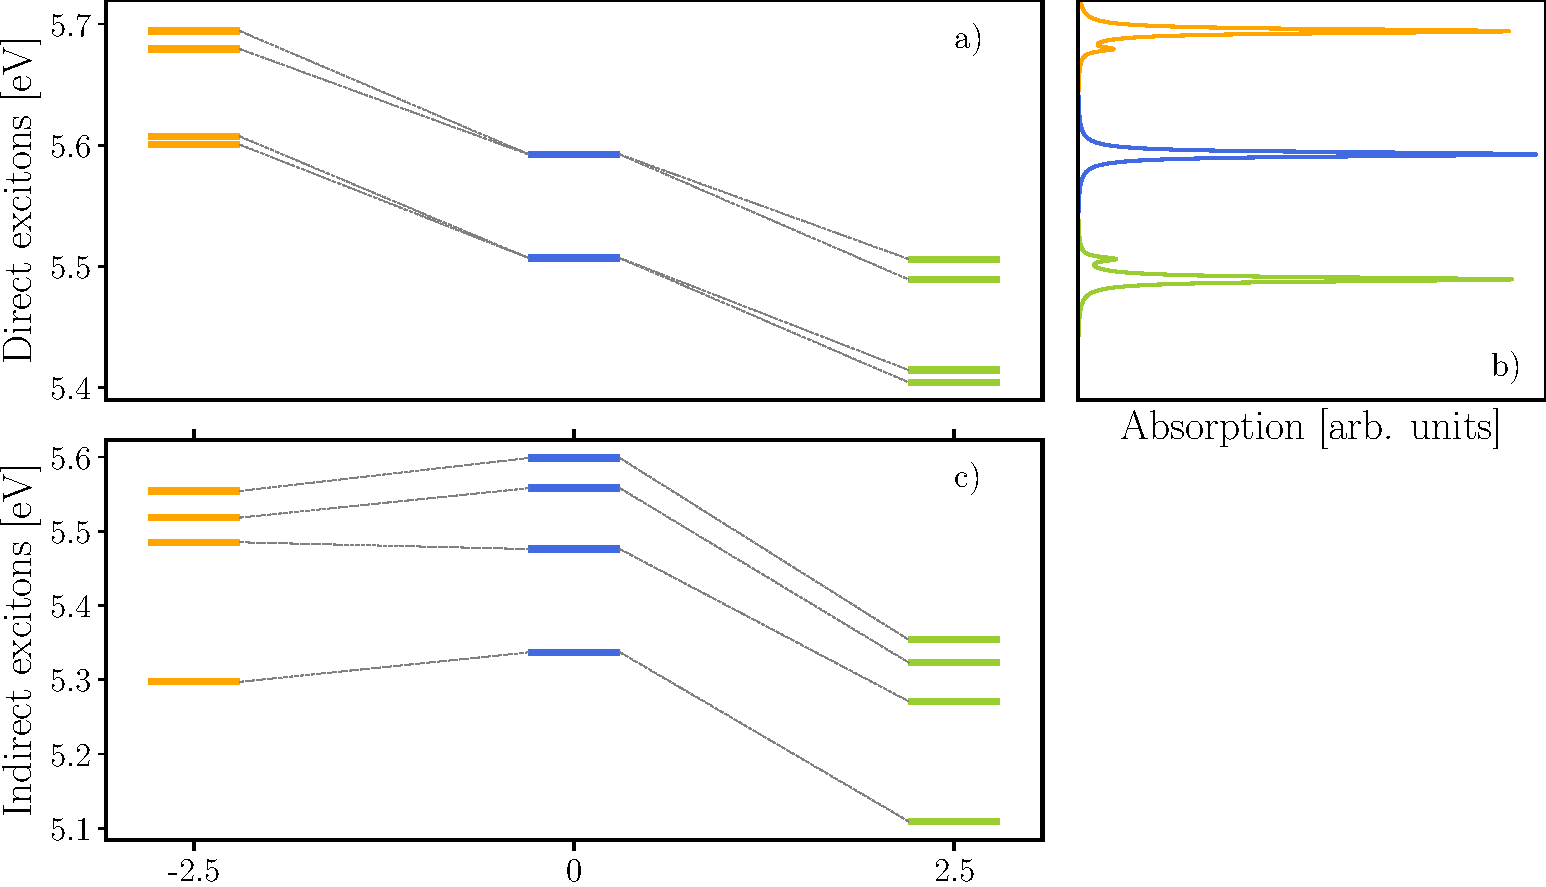
\includegraphics[width=0.8\textwidth]{hBN_exc_abs_vs_strain.pdf}
	\caption{Blue lines are for equilibrium crystal, orange is for compression and green is for stretch. (a) Energies of the lowest 4 excitons at $\Gamma$ (b) Absorption spectra associated with the direct excitons. Both excitons of the bright Davydov pair have a non-zero dipole matrix element and we can distinguish two peaks in the spectra for the strained crystals. (c) Energies of the lowest 4 indirect excitons.}
	\label{fig:exc_abs_vs_strain}
\end{figure}

The associated absorption spectra are displayed in panel (b) of Fig. \ref{fig:exc_abs_vs_strain}. As the inversion symmetry is not broken by uniaxial strain, the lowest two excitons remain dark when strain is applied. For the third and fourth lowest excitons in the strained systems, they are not mixed by the rotational symmetry as it is the case in the pristine crystal. This gives both excitons a non-zero dipole, and we see two peaks appearing in the absorption spectra. \\
The change of peak energy induced by strain is quantified by the strain gauge factor, which is defined as the spectral shift per \% of uniaxial strain. With these calculations, we find a value of $\approx$ 43 meV/\%, which is in the same range as transition metal dichalcogenides as reported in Ref. \cite{carrascoso2021strain}.

The splitting is also visible on the exciton wavefunctions in real space. It is displayed for the lowest two excitons at $\Gamma$, for a stretch of +2.5\%. The splitting is clear, with one of the wavefunctions having its components along the strained B-N bond or the armchair direction, while the other has its components along the zigzag direction.
\begin{figure}[tbp]
	\vspace{0.2cm}
	\setcapindent{2em}
	\centering
	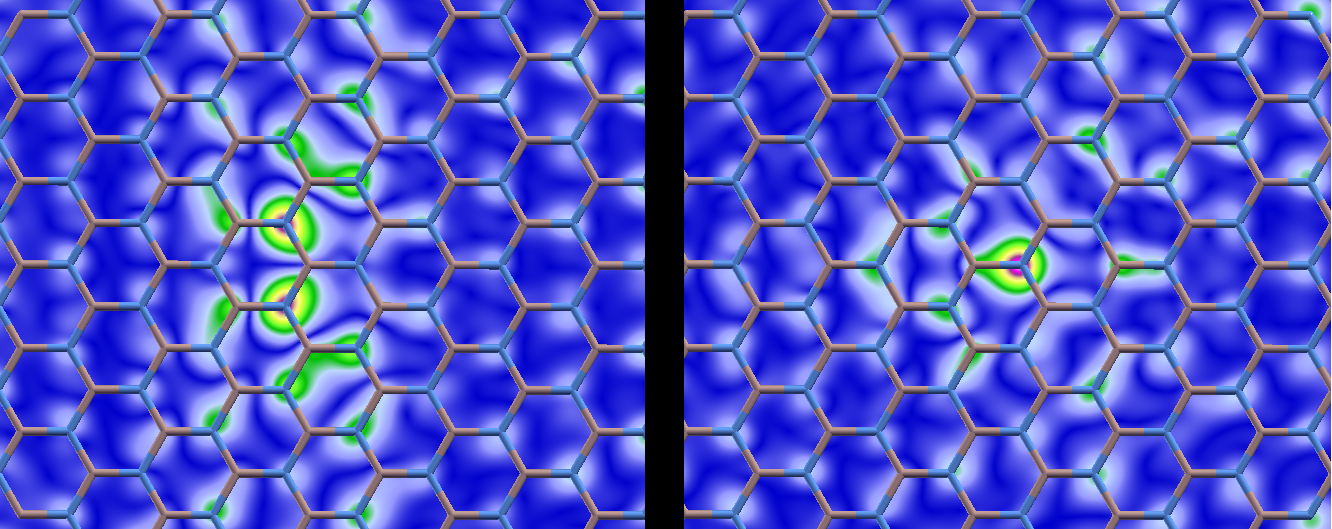
\includegraphics[width=0.8\textwidth]{excitonWF_strain.png}
	\caption{Electron distribution when the hole is fixed near the central Nitrogen atom, that we call exciton wavefunction. Left is the lowest dark exciton at $\Gamma$, right is the second lowest dark exciton at $\Gamma$, taken for a stretch of +2.5\%.}
	\label{fig:excWF_strain}
\end{figure}

We observe the same trend for the lowest-lying excitons with non-zero momentum, which we will call indirect excitons because they are formed by indirect electronic transitions. Their change in energy with strain is reported in Fig. \ref{fig:exc_abs_vs_strain} (c). It follows the same variation as the indirect gap and here again their binding energy is almost invariant with strain. The indirect excitons of hBN play an important role in light emission by luminescence. These changes in energy combined with the change in phonon frequencies will have an impact on the luminescence spectra of the strained crystals. This will be discussed in the next two sections.

%
\section{Exciton-phonon coupling from finite differences}
As presented in the introduction of the thesis, the inclusion of lattice vibrations in our computational framework is necessary to describe accurately the phonon-assisted features in the luminescence spectrum of hBN. In particular the exciton-phonon coupling is the central quantity to take into account. To do so, I present in this section how to calculate the macroscopic dielectric function with a static correction due to lattice vibrations, in a finite-difference scheme. The method can be found in Ref. \cite{paleari2019exciton} and in a slightly different approach in Ref. \cite{cannuccia2019theory}.\\
The key idea is to take the Taylor expansion of the macroscopic dielectric function with respect to atomic displacements. By displacing the atoms around their equilibrium positions along the phonon eigenvectors obtained earlier with \acrshort{DFPT} and calculating the response function with the \acrshort{BSE} in the displaced configurations, we will obtain the coupling between the exciton responsible for the optical response and the phonons. The link between the response function (without the long-range component) and the macroscopic dielectric function is given by Eq. \eqref{eq:eps_macro}. 
The Taylor exp is $\varepsilon (\omega)\approx \varepsilon^{(0)}(\omega) + \varepsilon^{st,(2)}_{\bar{q}}(\omega)$, where the second term is the static correction induced buy the atomic displacements.\cite{zacharias2016one} 
The contribution from exciton $\lambda$ to the response function  writes :
\begin{equation}
	\chi^\lambda_R(\omega) = \frac{|T^\lambda_R|^2}{E^\lambda_R - \omega + i \eta} \label{eq:chi_R_lambda}
\end{equation}
where the subscript R indicates that the quantities are evaluated at clamped ion positions. The infinitesimal $\eta$ is taken independent of $R$ for simplicity. Here we recall that we define the exciton dipole matrix element $T^\lambda = \sum_{cvk} \bar{A}_\lambda^{cvk} d_{cvk}$. The first derivative entering in the Taylor expansion will be :
\begin{equation}
	\frac{\partial \chi^\lambda_R(\omega)}{\partial R}\biggr|_{R=0} = \frac{\partial |T^\lambda_R|}{\partial R}\biggr|_{R=0} \frac{2|T^\lambda_{R=0}|}{E^\lambda_{R=0} - \omega + i\eta} + \frac{\partial \left[ E^\lambda_R - \omega + i\eta \right]^{-1}}{\partial R}\biggr|_{R=0} |T^\lambda_{R=0}|^2.
\end{equation}
This expression has a term linear in the exciton dipole and a term at the second power, both taken at clamped ion positions. It means that for dark excitons, the first derivative in the Taylor expansion will be zero. Excitons belonging in this category are labelled $\lambda'$, and we have $\frac{\partial \chi^{\lambda'}_R(\omega)}{\partial R}\bigr|_{R=0} = 0$.
In \acrshort{hBN}, the excitons involved in luminescence are the ones which low at the lowest energies in the dispersion, at finite momentum. Because of momentum conservation, these ones cannot recombine and emit light which has almost zero momentum, hence they are dark at clamped ion positions. Phonons are needed to transfer momentum and assist their recombination. \\ 
Similar arguments hold for the second derivative in the Taylor expansion
and the only non-vanishing term that remains is :
\begin{equation}
	\frac{\partial^2 \chi^{\lambda'}_R(\omega)}{\partial R^2} = \frac{\partial^2 |T^{\lambda'}_R|^2}{\partial R^2}\biggr|_{R=0} \left[ E^{\lambda'}_{R=0} - \omega + i\eta \right]^{-1} \label{eq:chi_fdd}
\end{equation}
This equation shows that it is equivalent to compute the finite-difference derivative of the full response function or only of the exciton dipoles. This is verified numerically in Ref. \cite{paleari2019exciton}. \\
This above second derivative is evaluated numerically with the finite difference formula :
\begin{equation}
	\frac{\partial^2 \chi^{\lambda'}_R(\omega)}{\partial R^2} \approx \frac{\chi(\Delta\RR;\omega) - 2 \chi_0(\omega) + \chi(-\Delta\RR;\omega)}{\Delta\RR^2}
\end{equation}
In our case, the displacements write $R \to R_{\mu\bar{q}}$ and are along the eigenvector of a particular phonon mode $\mu$ taken at the momentum $\bar{q}$ where the exciton dispersion reaches its minimum. The displacement magnitude are given by Eq. \eqref{eq:normal_displacements} taken for $t=0$ :
\begin{equation}
	u^{\mu\bar{q}}_{Ls\alpha}(t=0) = \frac{c}{\sqrt{M_s}}\Re\left\{ e^{i\bar{\qq}\cdot\boldsymbol{\tau}_L} \xi^{\mu\bar{q}}_{s\alpha} \right\}
\end{equation}
The $c$ parameter is a scaling factor which needs to be converged. Indeed for the finite difference derivative, we want to keep the displacements as small as possible. However if they are too small, their effect will be indistinguishable from numerical noise, but if they are too large, effects beyond the second-order derivatives will start to appear. For this work, we converged the displacements to a value of $|\Delta \RR| = 0.05 \AA$.
To accommodate the periodicity of the phonon at $\bar{q}$, we construct supercells. The supercell with the minimal size is non-diagonal,\cite{lloyd2015lattice} and we build them using the \texttt{yambopy} Python tool.\cite{Sangalli_2019}\\
From Ref. \cite{zacharias2020theory}, the second-order correction to the full dielectric due to the transitions assisted by a single phonon of momentum $\bar{q}$ is :
\begin{equation}
	\varepsilon^{st,(2)}_{\bar{q}} (\omega) = \frac{1}{2} \sum_\mu \left[ \sum_i^{N_{\bar{q}}} \frac{1}{2} \sum_j^2 \frac{\partial^2 \varepsilon^{(0)}_j(\omega)}{\partial R^2_{\mu\bar{q}}} \biggr|_{eq} \right] \sigma^2_{\mu\bar{q}} \label{eq:eps_Taylor_2nd}
\end{equation}
where $j$ is the polarization direction of the incoming light. We average over two orthogonal in-plane directions. The index $i$ runs over the equivalent $\bar{q}$ points in the \acrshort{BZ} where the exciton energies are minimal. For a perfect hBN crystal, $N_{\bar{q}} = 6$ but in our case, $N_{\bar{q}} = 4$. The last factor $\sigma^2_{\mu\bar{q}}$ is the thermal average of the squared displacement of the a quantum harmonic oscillator, given by :
\begin{equation}
	\sigma^2_{\mu\bar{q}}(T) = l^2_{\mu\bar{q}} (2n_{\mu\bar{q}}(T) + 1).
\end{equation}
$n_{\mu\bar{q}}(T)$ is the Bose-Einstein occupation function, and $l^2_{\mu\bar{q}} = 1/(2M_{\mu\bar{q}}\Omega_{\mu\bar{q}})$ is the zero-temperature squared displacement (from now on we refer to phonon frequencies with capital Omega). In our case the reference mass is $M_{\mu\bar{q}} = \sum^{N_{ions}}_s M_s |\xi_s^{\mu\bar{q}}|^2$.\\
Finally the imaginary part of the dielectric function follows from Eqs. \eqref{eq:chi_fdd},\eqref{eq:chi_R_lambda} and \eqref{eq:eps_macro} : 
\begin{equation}
	\Im\frac{\partial^2 \varepsilon^{(0)}(\omega)}{\partial R^2_{\mu\bar{q}}}\biggr|_{eq} = \frac{8\pi}{N_k V} \sum_{\lambda'} \frac{\partial^2 |T^{\lambda'}|^2}{\partial R^2_{\mu\bar{q}}}\biggr|_{eq} \Im\left\{ \frac{1}{\omega - E^{\lambda'} + i\eta} \right\}.
\end{equation}
At this point we can reintroduce the dependence on the phonon frequency coming from the energy conservation in perturbation theory, which was neglected above (more details can be found in Ref. \cite{paleari2019first}). Two terms appear, one coming from the process of phonon emission which is proportional to $1 + n_{\mu\bar{q}}$ and one from phonon absorption proportional to $n_{\mu\bar{q}}$. At low temperature, $1 \gg n_{\mu\bar{q}}$ which means that absorbing a phonon is much less likely than emitting one. We have the transformation :
\begin{equation}
	\frac{2n_{\mu\bar{q}} + 1}{\omega - E^{\lambda'} + i\eta} \to \frac{n_{\mu\bar{q}} + 1}{\omega - E^{\lambda'} - \Omega_{\mu\bar{q}} + i\eta} + \frac{n_{\mu\bar{q}}}{\omega - E^{\lambda'} + \Omega_{\mu\bar{q}} + i\eta}
\end{equation}
Finally, similarly to Ref \cite{paleari2019exciton}, we rename the numerator between square brackets in Eq. \eqref{eq:eps_Taylor_2nd} as $|t^{\text{static}}_{\mu\bar{q}\lambda'}|^2$. It represents the static formation probability of an exciton $\lambda'$ mediated by a phonon mode $\mu$ with momentum $\bar{q}$ and frequency $\Omega_{\mu\bar{q}}$. We can call this quantity \textit{exciton-phonon coupling} matrix element in the sense of optical absorption and exciton creation. This is to be compared with the exciton-phonon matrix elements obtained \textit{ab initio} in Chapter 3.\\
The final expression writes :
\begin{equation}
	\varepsilon^{(2)}_{\bar{q}2}(\omega) = \sum_{\lambda\lambda'} |t^{\text{static}}_{\mu\bar{q}\lambda'}|^2 l^2_{\mu\bar{q}} \left[ n_{\mu\bar{q}} + 1/2 \mp 1/2 \right] \delta(\omega - E^{\lambda'} \pm \Omega_{\mu\bar{q}}). \label{eq:eps2_fdd}
\end{equation}
The upper (lower) sign refers to the process of phonon absorption (emission). One thing to note here is that we neglect the variation of the exciton energies induced by the coupling with phonon. This is justified for hBN because the exciton energies are large enough compared to this renormalization, and moreover we know that the $GW$ approximation underestimates the fundamental gap, so the energies we will obtain at the end of the process will not be accurate anyways. Instead, we focus on obtaining spectra that reproduce the shape of phonon-assisted replicas.

%
\section{Luminescence results}
We used the expression of the dielectric function in Eq. \eqref{eq:eps2_fdd} and plugged it in the van Roosbroeck--Shockley relation from Eq. \eqref{eq:vRS_PL_ind}. The full expression writes :
\begin{multline}
	R^{sp}(\omega)= \sum_{\mu,{\bar{q}}} \frac{\omega(\omega + 2\Omega_{\mu \bar{q}})^2}{\pi^2 c^3 } n_1(\omega) \sum_S \frac{\partial^2 |T^{\lambda'}|^2 }{\partial R_{\mu\bar{q}}^2}\biggr|_{\text{eq}} \\ \times	\Im \left\{\frac{1}{\omega-(E^{\lambda'}-\Omega_{\mu \bar{q}})+i\eta}\right\} n_B(E^{\lambda'}_{\bar{q}},T_{exc})
\end{multline}
where $n_B(E^{\lambda'}_{\bar{q}},T_{exc}) = e^{-(E^{\lambda'}-E^{min})/k_BT_{exc}}$ is the Boltzmann occupation for excitons where the energy difference is taken with the minimal exciton energy over the whole Brillouin Zone $E^{min}$. It means that the lowest valleys in the exciton dispersion will be populated by relaxed excitons, while the higher states will have exponentially decaying populations. For instance, the direct exciton has an energy too large to even be visible in the spectrum.
As discussed above, we simulate a crystal at low temperature, which we set at 10K in agreement with the experimental measurements. Hence we approximated $1 + n_{\mu\bar{q}} \approx 1$, and we neglect the phonon absorption processes, which would give higher energy peaks that would be suppressed by the Boltzmann function anyway. The excitonic temperature $T_{exc}$ is higher than the lattice temperature because we consider a steady-state process in which the excitons do not thermalize, since they are constantly pumped by the laser. We obtained the value by fitting the experimental data of Ref. \cite{cassabois2016hexagonal} which gave us the value of $T_{exc} = 24 K$ for a lattice temperature of $T_L = 10 K$. The effect of temperature is also taken into account in the broadening parameter of the peaks with the Lorentzian model : $\eta = \Gamma_0 + aT + bB(T)$ where the values of the parameters can be found in Refs. \cite{paleari2019exciton,vuong2017exciton}. Another approximation we made is to compute the dipoles at the displaced configurations with the statically screened interaction from the equilibrium configurations : 
\begin{equation}
	\frac{\partial^2 |T^{\lambda'} (W, L )|^2 }{\partial R_{\mu \bar{q}}^2} \simeq \frac{\partial^2 |T^{\lambda'} (W(R=R_{eq}), L) |^2 }{\partial R_{\mu \bar{q}}^2}.
\end{equation}
It has been shown previously that this has negligible effects for the calculation of electron-phonon matrix elements,\cite{faber2015exploring} and we verified that our results are not modified by this approximation. 

Now comes the discussion about the choice of $\bar{q}$. For the pristine hBN crystal, the indirect electronic gap is between two points close to the \KK~point and the \MM~point. The usual approximation is to consider that the gap lies on the \KK~point, and that the momentum that connects the two points is $\qq = (\tfrac{1}{3}, -\tfrac{1}{6}, 0)$ and that the minimum of the exciton dispersion is also at this momentum. This simplifies the construction of the supercells needed to accommodate the phonon modes at this $\qq$-vector. In our case, because of the symmetry breaking in the electronic dispersion, there are several indirect gaps which have a very similar energy, especially for low values of strain. This could lead to a broadening of the peaks in the luminescence spectra. In order to verify this hypothesis, we constructed the supercells which accommodate all the vectors corresponding to the transitions $\bf M - \bf K$,  $\bf M - \bf {K'}$,  $\bf {M'} - \bf K$ , $\bf {M'}  - \bf { K'}$. Then we performed a \acrshort{BSE} calculation for all these non-diagonal supercells containing 24 displaced atoms and summed the dipoles. Because of the displacement of atoms, some symmetries are broken and the dark excitons which are folded at $\Gamma$ acquire a finite dipole, hence contributing to the luminescence spectra.\\

The resulting spectra for various values of strained are displayed in Fig. \ref{fig:Lum_vs_strain}.
\begin{figure}[tbp]
	\vspace{0.2cm}
	\setcapindent{2em}
	\centering
	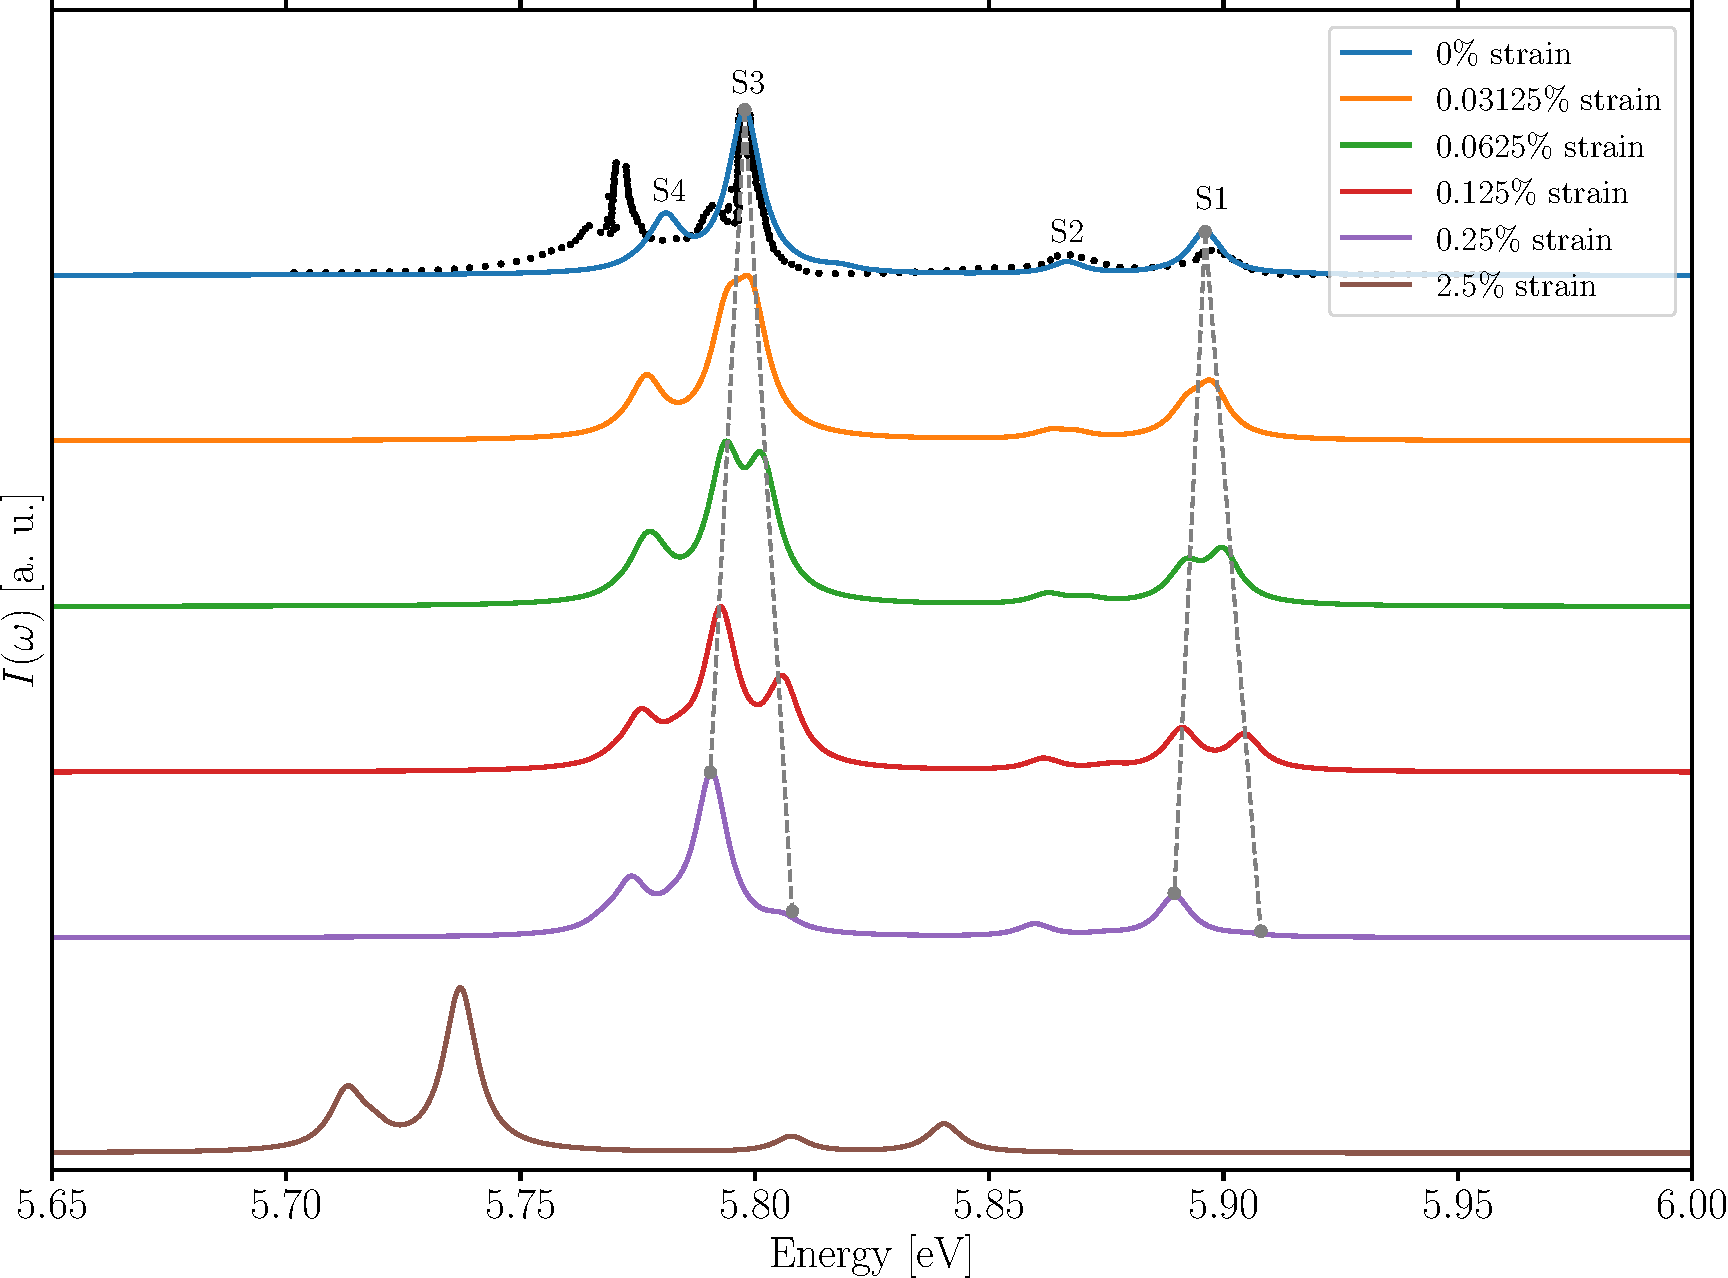
\includegraphics[width=0.9\textwidth]{Lum_vs_strain.pdf}
	\caption{Luminescence spectra as a function of strain, for selected value of compressive strain. Plots are shifted vertically for clarity. On the top plot, experimental data is represented by the black dots from Ref. \cite{schue2019bright}. The spectra have been shifted to match the position of the indirect exciton at equilibrium, and compensate the numerical error of the $GW$ approximation.\cite{artus2021ellipsometry} Dashed lines are a guide for the eye.}
	\label{fig:Lum_vs_strain}
\end{figure}
First, we can see on the top plot that the equilibrium luminescence spectrum is quite well reproduced compared to experiment. At low values of strain, the excitons originating from the different $\bf{ M^{(')}} - \bf{ K^{(')}}$ transitions have a very close energy and therefore all of them contribute to the luminescence spectra as they are not suppressed by the Boltzmann function. These excitons scatter with phonons who also have their frequencies modified. These combined effects create a splitting of the peaks which increases with strain. There is also a slight increase in the intensty of the S1 and S2 peaks, coming from scattering with LA and TA modes. At equilibrium, we found that the S3/S1 intensity ratio is $\approx 3.7$ and it decreases down to $\approx 2.7$ with strain. This result is in line with those of Léonard Schué in Ref. \cite{schue2017proprietes}, however they found a ratio going down to $\approx 1$ in their compressed samples.\\ The discrepancy could be explained by the lack of the fine sampling of the exciton and phonon dispersions. Indeed with a larger density of states to scatter, the intensity of some peaks could be increased even more. The differences could also come from experimental factors not accounted for in our simulation methods, such as surface effects or non-uniform strain field.\\
Finally, for larger values of strain, the exciton energies split so much that the peaks coming from the higher one are suppressed by the Boltzmann function in the van Roosbroeck--Shockley relation. The spectrum thus acquires the same shape as the equilibrium one but translated to lower energies due to the closure of the indirect gap, and the change in the phonon frequencies. Note that the $2.5\%$ value of strain is extreme and is probably out of reach in the experimental conditions we try to reproduce. The results are similar for the tensile strain.

%
\section*{Conclusion of the chapter}
In this chapter, I presented our results about the electronic, phononic and optical properties of bulk hBN under uniaxial strain, both tensile and compressive., along the armchair direction. We observed a splitting of the exciton at $\Gamma$ due to the breaking
of the threefold rotational symmetry. This splitting could be measured in reflectivity experiments.\cite{elias2021flat} We also found that the direct excitons energies vary linearly with the applied strain, while the indirect exciton energies decrease both with compression and stretch. We were also able to evaluate the strain gauge factor, which was found to be similar to that of transition metal dichalcogenides.
I presented a method to include the exciton-phonon coupling in the response function and hence in the optical spectra of the strained crystals. It is based on a finite-difference derivative approach and is well-suited for materials with a indirect and deep exciton dispersion exciton minimum. The coupling of excitons and phonons is calculated only for a few momenta in the Brillouin Zone. Since this method requires the use of supercells, it is particularly adapted to the study of defects such as in Ref. \cite{libbi2022phonon}. We employed the method to compute the phonon-assisted luminescence spectrum and how it changes with strain. We found that at low strain,additional peaks appear in the spectra due to the breaking of the degeneracy between the different \KK~ and \MM~ points in the Brillouin Zone. These additional peaks decrease the intensity ratio between the acoustic- and the optical-phonon assisted transitions, in agreement with recent measurements. For large compressive strain we found that only one valley contributes to the luminescence, and the spectra return to a shape similar to the equilibrium one but shifted at lower energies. This prediction could be verified by means of luminescence measurements in highly strained h-BN.\cite{blundo2022vibrational}

	\chapter{Ab initio exciton-phonon coupling}
\chaptertoc{}

\section{Introduction}
Mainly on monolayer, the three experiments
mention also the cathodoluminescence paper in which we see only the direct peak
say we did a benchmark on hBN
talk about the bBN and the reason we chose it : direct and indirect gaps are close in energy so we might see direct peak and phonon satellites. Indeed it was see experimentally so it is a good candidate for our method.

\section{monolayer exciton dispersion}
fitting of the dispersion, Lbar vs Lfull
the nearly-free electron states at Gamma

\section{Theory of the ab initio exciton-phonon coupling}
The derivation in MBPT is carried out in Pierluigi Cuddazzo's paper in 2020 and with extensive details in Fulvio's thesis. Here we follow a different approach, similar to Chen's derivation. I should mention the fact that they compute the exc-ph matrix elements like us, but the luminescence is different.\\
For simplicity, drop $\QQ$.
exciton creation and annihilation operators\\

We consider a system with displacements from the equilibrium positions $\boldsymbol{u}_{Ls}$ ($L$ labels the unit cell and $s$ the atom). Taylor expansion of the Kohn-Sham potential around the equilibrium positions :
\begin{equation}
    V^{KS}(\left\{ \uu_{Ls} \right\}) = V_0^{KS} + \sum_{Ls\alpha} \frac{\partial V^{KS}}{\partial \uu_{Ls\alpha}} \uu_{Ls\alpha} + \mathcal{O}(\left\{ \uu_{Ls} \right\}^2)
\end{equation}
The electronic wave functions and eigenvalues of the perturbed system depend on the atomic displacements $\left\{ \uu_{Ls} \right\}$. To obtain their change in the perturbed system, we apply first-order perturbation theory by keeping terms linear in $\left\{ \uu_{Ls} \right\}$. To first order, the correction to the eigenvalues vanishes while the correction to the Kohn-Sham wave functions $\psi_i$, (solutions of Eq. \eqref{eq:KS_eqs}) can be written as : 
\begin{equation}
    \delta\ket{\psi_i} = \sum_{j\neq i} \frac{\bra{\psi_j} \Delta V \ket{\psi_i}}{\epsilon_i - \epsilon_j} \ket{\psi_j}, \qquad \text{with} \ \ \Delta V = \sum_{Ls\alpha}\frac{\partial V^{KS}}{\partial \uu_{Ls}}\cdot \uu_{Ls}
\end{equation}
In the following, we use the tilde for quantities of the perturbed system and write the perturbed wave function as :
\begin{equation}
    \ket{\tilde{\psi}_i} = \ket{\psi_i} + \delta\ket{\psi_i} = \ket{\psi_i} + \sum_{j \neq i} \Delta_{ij} \ket{\psi_j}
\end{equation}
with
\begin{equation}
    \Delta_{ij} \equiv \frac{\bra{\psi_j} \Delta V \ket{\psi_i}}{\epsilon_i - \epsilon_j}
\end{equation}

We start by defining an unpertubed Bethe-Salpeter Hamiltonian $H \equiv H(\{\boldsymbol{u}_{Ls} \}=0)$ and a perturbed BSE Hamiltonian $\Tilde{H} \equiv H(\{\boldsymbol{u}_{Ls} \})$. We will use first order perturbation theory to obtain the exciton-phonon interaction. The BSE Hamiltonian writes :
\begin{equation}
    H_{vc,v'c'} = \bra{vc} H \ket{v'c'} = ( \epsilon_c - \epsilon_v ) \delta_{vv'}\delta_{cc'} + K_{vc,v'c'}
    \label{eq:BSE_H}
\end{equation}
where $c,v$ are for conduction and valence band, respectively. The perturbed Hamiltonian one is :
\begin{equation}
    \Tilde{H}_{\Tilde{v}\Tilde{c},\Tilde{v}'\Tilde{c}'}  = \bra{\Tilde{v}\Tilde{c}} H \ket{\Tilde{v}'\Tilde{c}'}  = ( \Tilde{\epsilon}_c - \Tilde{\epsilon}_v ) \delta_{\Tilde{v}\Tilde{v}'}\delta_{\Tilde{c}\Tilde{c}'} + K_{\Tilde{v}\Tilde{c},\Tilde{v}'\Tilde{c}'}
\end{equation}
The Bethe-Salpeter kernel is defined as :
\begin{equation}
    K_{vc,v'c'} = \bra{vc} K \ket{v'c'} = \int d1 d2 d3 d4 \psi_v(2) \psi_c^*(1) K(1234) \psi^*_{v'}(3)\psi_{c'}(4)
\end{equation}
where
\begin{equation}
    K(1234) = -i\delta(1,2)\delta(3,4)\ v(1,4) + i \delta(1,4)\delta(2,3)\ W(1,2)
\end{equation}
with $v$ being the bare Coulomb potential and $W$ the screened Coulomb interaction. In the fashion of Many-Body theory, space, time and spin variables are grouped like so : $1 = (\boldsymbol{r_1},t_1,\sigma_1)$. $\Tilde{K}_{\Tilde{v}\Tilde{c},\Tilde{v}'\Tilde{c}'}$ is the 
\begin{equation}
    \Tilde{K}_{\Tilde{v}\Tilde{c},\Tilde{v}'\Tilde{c}'} = \bra{\Tilde{v}\Tilde{c}} \Tilde{K} \ket{\Tilde{v}'\Tilde{c}'} 
\end{equation}
Solving the BSE Hamiltonian in \eqref{eq:BSE_H} gives the exciton wave functions $\ket{S_n}$ and energies $E^{S_n}$ :
\begin{align}
    \sum_{v',c'} H_{vc,v'c'} A^{S_n}_{v'c'} &= E^{S_n} A^{S_n}_{vc} \\
    \ket{S_n} = \sum_{vc}& A_{vc}^{S_n}\ket{vc}
\end{align}
To derive the exciton-phonon interaction, we project the perturbed BSE Hamiltonian onto the unperturbed basis set and keep only the terms to first-order in the phonon perturbation. By such a process, the terms that will arise and be different from the unperturbed BSE Hamiltonian will define the exciton-phonon interaction. One can show that to first order, the perturbed and unperturbed electronic energies coincide, so we will use $\Tilde{\epsilon}_i = \epsilon_i$. The perturbed Hamiltonian in the unperturbed basis is :
\begin{align*}
    \Tilde{H}_{nm} = \bra{S_m} \Tilde{H} \ket{S_n} &= \sum_{\Tilde{v}\Tilde{c},\Tilde{v}'\Tilde{c}'}  \bra{S_m}\ket{\Tilde{v}\Tilde{c}}\bra{\Tilde{v}\Tilde{c}} \Tilde{H} \ket{\Tilde{v}'\Tilde{c}'}\bra{\Tilde{v}'\Tilde{c}'}\ket{S_n} \\
    &= \sum_{vc,v'c'}\sum_{\Tilde{v}\Tilde{c},\Tilde{v}'\Tilde{c}'} \bra{S_m}\ket{vc}\bra{vc}\ket{\Tilde{v}\Tilde{c}}\bra{\Tilde{v}\Tilde{c}} \Tilde{H} \ket{\Tilde{v}'\Tilde{c}'}\bra{\Tilde{v}'\Tilde{c}'}\ket{v'c'}\bra{v'c'}\ket{S_n}
\end{align*}
where we used the completeness relations of both basis sets, $\sum_{vc}\ket{vc}\bra{vc} = 1$ and $\sum_{\Tilde{v},\Tilde{c}} \ket{\Tilde{v}\Tilde{c}}\bra{\Tilde{v}\Tilde{c}} = 1$. By definition of the BSE wave functions $\bra{v'c'}\ket{S_n} = A^{S_n}_{v'c'}$, then we can write the above equation as :
\begin{equation}
    \Tilde{H}_{nm} = \bra{S_m} \Tilde{H} \ket{S_n} = \sum_{vc,v'c'} A{^S_m *}_{vc} A^{S_n}_{v'c'} \times \left[ \sum_{\Tilde{v}\Tilde{c},\Tilde{v}'\Tilde{c}'} \bra{vc}\ket{\Tilde{v}\Tilde{c}}  \bra{\Tilde{v}\Tilde{c}} \Tilde{H} \ket{\Tilde{v}'\Tilde{c}'} \bra{\Tilde{v}'\Tilde{c}'}\ket{v'c'} \right]
    \label{eq:exc_ham}
\end{equation}
The term inside the square brackets can be separated into to terms :
\begin{align*}
    &\sum_{\Tilde{v}\Tilde{c},\Tilde{v}'\Tilde{c}'} \bra{vc}\ket{\Tilde{v}\Tilde{c}}  \bra{\Tilde{v}\Tilde{c}} \Tilde{H} \ket{\Tilde{v}'\Tilde{c}'} \bra{\Tilde{v}'\Tilde{c}'}\ket{v'c'} =  \sum_{\Tilde{v}\Tilde{c},\Tilde{v}'\Tilde{c}'} \bra{vc}\ket{\Tilde{v}\Tilde{c}}  \left[ (\Tilde{\epsilon}_{\Tilde{c}} - \Tilde{\epsilon}_{\Tilde{v}}) \delta_{\Tilde{v}\Tilde{v}'}\delta_{\Tilde{c}\Tilde{c}'} + \Tilde{K}_{\Tilde{v}\Tilde{c},\Tilde{v}'\Tilde{c}'} \right] \bra{\Tilde{v}'\Tilde{c}'}\ket{v'c'} \\
    &= \sum_{\Tilde{v}\Tilde{c}} \bra{vc}\ket{\Tilde{v}\Tilde{c}} (\epsilon_{\Tilde{c}} - \epsilon_{\Tilde{v}}) \bra{\Tilde{v}\Tilde{c}}\ket{v'c'} + \sum_{\Tilde{v}\Tilde{c},\Tilde{v}'\Tilde{c}'} \bra{vc}\ket{\Tilde{v}\Tilde{c}} \Tilde{K}_{\Tilde{v}\Tilde{c},\Tilde{v}'\Tilde{c}'} \bra{\Tilde{v}'\Tilde{c}'}\ket{v'c'}
\end{align*}
We make the choice to approximate the perturbed kernel with the unperturbed one, $\Tilde{K}_{\Tilde{v}\Tilde{c},\Tilde{v}'\Tilde{c}'} \approx \bra{\Tilde{v}\Tilde{c}}K\ket{\Tilde{v}'\Tilde{c}'}$, that is to say the effect of the atomic displacements on the bare and screened Coulomb interactions can be neglected and $W \approx \Tilde{W}$. With this approximation we have :
\begin{equation}
    \sum_{\Tilde{v}\Tilde{c},\Tilde{v}'\Tilde{c}'} \bra{vc}\ket{\Tilde{v}\Tilde{c}} \Tilde{K}_{\Tilde{v}\Tilde{c},\Tilde{v}'\Tilde{c}'} \bra{\Tilde{v}'\Tilde{c}'}\ket{v'c'} 
    \approx  \sum_{\Tilde{v}\Tilde{c},\Tilde{v}'\Tilde{c}'} \bra{vc}\ket{\Tilde{v}\Tilde{c}} 
    \bra{\Tilde{v}\Tilde{c}} K \ket{\Tilde{v}'\Tilde{c}'}\bra{\Tilde{v}'\Tilde{c}'}\ket{v'c'} = \bra{vc} K \ket{v'c'} = K_{vc,v'c'}
\end{equation}
and thus the term in brackets in Eq. \eqref{eq:exc_ham} becomes 
\begin{equation}
    \sum_{\Tilde{v}\Tilde{c},\Tilde{v}'\Tilde{c}'} \bra{vc}\ket{\Tilde{v}\Tilde{c}}  \bra{\Tilde{v}\Tilde{c}} \Tilde{H} \ket{\Tilde{v}'\Tilde{c}'} \bra{\Tilde{v}'\Tilde{c}'}\ket{v'c'} = \sum_{\Tilde{v}\Tilde{c}} \bra{vc}\ket{\Tilde{v}\Tilde{c}} (\epsilon_{\Tilde{v}} - \epsilon_{\Tilde{c}}) \bra{\Tilde{v}\Tilde{c}}\ket{v'c'} +  K_{vc,v'c'} 
\end{equation}
Next, we use Eq. (pas écrite) to expand $\sum_{\Tilde{v}\tilde{c}} \bra{vc}\ket{\Tilde{v}\Tilde{c}} (\epsilon_{\Tilde{c}} - \epsilon_{\Tilde{v}})\bra{\Tilde{v}\Tilde{c}}\ket{v'c'}$ to order $\mathcal{O}(\Delta)$. We work within the Tamm-Dancoff approximation and keep only the resonant part of the BSE Hamiltonian; as a consequence, only valence-valence and conduction-conduction hole- and electron-phonon are allowed, that is to day $\Delta_{vc} = \Delta_{cv} = 0$. Using Eq. (pas écrite) we get :
\begin{align}
\begin{split}
    \bra{vc}\ket{\tv\tc} &= \bra{v}\ket{\tv}\bra{c}\ket{\tc} = \left(\delta_{v\tv} + \sum_{v''\neq\tv}\Delta_{\tv v''}\delta_{vv''}\right) \left(\delta_{c\tc} + \sum_{c''\neq \tc}\Delta_{\tc c''}\delta_{cc''}\right) \\
    &= \left( \delta_{v\tv}\delta_{c\tc} + \delta_{v\tv} \sum_{c''\neq\tc} \Delta_{\tc c''}\delta_{cc''} + \delta_{c\tc}\sum_{v''\neq \tv} \Delta_{\tv v''} \delta_{vv''} \right) + \mathcal{O}(\Delta^2)
\end{split}
\end{align}
and similarly
\begin{equation}
    \bra{\tv\tc}\ket{v'c'} = \bra{v'}\ket{\tv}^*\bra{c'}\ket{\tc}^* = \left( \delta_{v'\tv}\delta_{c'\tc} + \delta_{v'\tv} \sum_{c''\neq\tc} \Delta^*_{\tc c''}\delta_{c'c''} + \delta_{c'\tc}\sum_{v''\neq \tv} \Delta^*_{\tv v''} \delta_{v'v''}  \right)  + \mathcal{O}(\Delta^2)
\end{equation}
With these expressions, there are five first-order terms in $\sum_{\Tilde{v}\tilde{c}} \bra{vc}\ket{\Tilde{v}\Tilde{c}} (\epsilon_{\Tilde{c}} - \epsilon_{\Tilde{v}})\bra{\Tilde{v}\Tilde{c}}\ket{v'c'}$ that we can simplify using the Kronecker delta :
\begin{align}
    \sum_{\tv\tc} \bra{vc}\ket{\tv\tc} (\epsilon_{\Tilde{c}} - \epsilon_{\Tilde{v}})\bra{\tv\tc}\ket{v'c'} \nonumber \\
    %
        \approx (\epsilon_c - \epsilon_v)\delta_{vv'}\delta_{cc'} &+ \delta_{cc'}\sum_{\tv}(\epsilon_c - \epsilon_{\tv}) \sum_{v''\neq \tv} (\Delta^*_{\tv v''}\delta_{vv''}\delta_{v'\tv} + \Delta_{\tv v''}\delta_{v'v''}\delta_{v\tv}) \nonumber \\
        &+  \delta_{vv'} \sum_{\tc} (\epsilon_{\tc} - \epsilon_v) \sum_{c'' \neq\tc} (\Delta_{\tc c''}\delta_{cc''}\delta_{c'\tc} + \Delta^*_{\tc c''}\delta_{c'c''}\delta_{c\tc}) \nonumber \\
        %
        = (\epsilon_c - \epsilon_v)\delta_{vv'}\delta_{cc'} &+ \delta_{cc'} \left[  \sum_{v''\neq v'} (\epsilon_c - \epsilon_{v'}) \Delta^*_{v'v''}\delta_{v v''} + \sum_{v'' \neq v} (\epsilon_c - \epsilon_v) \Delta_{vv''} \delta_{v'v''} \right] \nonumber \\
        &+  \delta_{vv'} \left[ \sum_{c''\neq c'} (\epsilon_{c'} - \epsilon_v)\Delta_{c' c''}\delta_{cc''} + \sum_{c''\neq c} (\epsilon_c - \epsilon_v) \Delta^*_{cc''}\delta_{c'c''} \right] \nonumber \\
    %
    = (\epsilon_c - \epsilon_v) \delta_{vv'}\delta_{cc'} &+ \delta_{cc'}(\epsilon_{v'} - \epsilon_v) \Delta_{vv'} + \delta_{vv'}(\epsilon_c - \epsilon_{c'}) \Delta^*_{cc'}
\end{align}
where we used $\Delta_{ij} = -\Delta_{ji}^*$ to obtain the last line. Finally, the perturbed Hamiltonian in the excitonic basis in Eq. \eqref{eq:exc_ham} becomes :
\begin{align}
    \tilde{H}_{mn} &= \sum_{vc,v'c'} A^{S_m *}_{vc} A^{S_n}_{v'c'} \times \left\{ \left[ (\epsilon_c - \epsilon_v) \delta_{vv'}\delta_{cc'} + K_{vc,v'c'} \right] + \delta_{cc'} (\epsilon_{v'} - \epsilon_v)\Delta_{vv'} + \delta_{vv'}(\epsilon_c - \epsilon_{c'}) \Delta_{cc'}^*  \right\} \nonumber \\
    &= E^{S_m}\delta_{mn} + \sum_{vc,v'c'} A^{S_m*}_{vc} A^{S_n}_{v'c'} \cdot \left( \delta_{cc'}(\epsilon_{v'} - \epsilon_v) \Delta_{vv'}  + \delta_{vv'} (\epsilon_c - \epsilon_{c'}) \Delta^*_{cc'} \right) \label{eq:perturb_H_exc}
\end{align}
where we use the fact that the unperturbed Hamiltonian is diagonalized by the Tamm-Dancoff exciton eigenvectors :
\begin{equation}
    E^{S_m}\delta_{mn} = \sum_{vc,v'c'} A^{S_m*}_{vc} A^{S_n}_{v'c'} \times \left( (\epsilon_c - \epsilon_v)\delta_{vv'}\delta_{cc'}+ K_{vc,v'c'} \right).
\end{equation}
Therefore, the first term in the second line of Eq. \eqref{eq:perturb_H_exc} is the unperturbed Hamiltonian, while the second term is the exciton-phonon interaction,
\begin{equation}
    \tilde{H}_{\text{exc-ph}} = \sum_{vc,v'c'} A^{S_m*}_{vc} A^{S_n}_{v'c'} \cdot \left( \delta_{cc'}(\epsilon_{v'} - \epsilon_v) \Delta_{vv'}  + \delta_{vv'} (\epsilon_c - \epsilon_{c'}) \Delta^*_{cc'} \right). \label{eq:H_exc-ph}
\end{equation}
To obtain the final result, we reintroduce the momemtum dependence and the Bloch states :
\begin{equation}
    \ket{\phi_i} \to \ket{\phi_{n\kk}}
\end{equation}
and the transition basis set for an exciton with center of mass momentum $\QQ$ is $\ket{vc} = \ket{v\kk_v,c\kk_c} = \ket{v\kk_v,c\kk_v + \QQ}$. We write the change in potential due to atomic displacements using normal coordinates :
\begin{equation}
    \Delta V = \sum_{\mu \qq} \sqrt{\frac{1}{2\Omega_{\mu\qq}}} \Delta_{\mu\qq} V^{KS}(\hat{b}_{\mu\qq} + \hat{b}^\dagger_{\mu-\qq})  
\end{equation}
Then the $\Delta_{ij}$ describing the transition from $i$-th to $j$-th state becomes :
\begin{equation}
    \Delta_{n\kk n'\kk'} = \frac{\bra{n'\kk'} \Delta V \ket{n\kk}}{\epsilon_{n\kk} - \epsilon_{n'\kk'}} = \sum_{\mu\qq} \frac{g_{nn'v}(\kk,\qq) \delta(\kk'-\kk-\qq)}{\epsilon_{n\kk} - \epsilon_{n'\kk'}} (\hat{b}_{\mu\qq} + \hat{b}^\dagger_{\mu-\qq})
\end{equation}
where $g_{nn'\mu}(\kk,\qq) = (1/2\Omega_{\mu\qq})^{1/2} \bra{n'\kk'} \Delta_{\mu\qq} V^{KS} \ket{n\kk}$ is the usual electron-phonon matrix element \textcolor{red}{check if it corresponds to the expression I gave in chapt1}, namely the probability amplitude for an electron in band $n$ with crystal momentum $\kk$ to transition to a final state in band $n'$ and momentum $\kk' = \kk+\qq$ by absorbing or emitting a phonon with mode index $\mu$ and wave vector $\qq$.

By introducing exciton creation and annihilation operators, $\hat{a}^\dagger_{S_n(\QQ)}$ and $\hat{a}_{S_n(\QQ)}$, we rewrite the exciton-phonon interaction from Eq. \eqref{eq:H_exc-ph} as :
\begin{equation}
    \tilde{H}_{\text{exc-ph}} = \sum_{mn\mu, \QQ\qq} \mathcal{G}_{mn\mu}(\QQ,\qq) \hat{a}^\dagger_{S_n(\QQ+\qq)} \hat{a}_{S_n(\QQ)} (\hat{b}_{\mu\qq} + \hat{b}^\dagger_{\mu-\qq}).
\end{equation}
where we defined the exciton-phonon matrix elements as :
\begin{multline}
    \mathcal{G}_{nm\mu}(\QQ,\qq) = \sum_{\substack{vcv'c'\\ \kk_v \kk_c \kk'_{v'} \kk'_{c'}}} A^{S_m(\QQ+\qq)*}_{v\kk_v,c\kk_c} A^{S_n(\QQ)}_{v'\kk'_{v'},c'\kk'_{c'}} \left[ \delta_{vv'} g_{c'c\mu}(\kk'_{c'},\qq) \delta(\kk_c - \kk'_{c'} - \qq) \right. \\
    \left. - \delta_{cc'}g_{vv'\mu}(\kk_v,\qq) \delta(\kk'_{v'} - \kk_v -\qq) \right]. \label{eq:Gkkp}
\end{multline}
Let us make momentum conservation explicit to obtain the final expression. The exciton-phonon coupling constant $\mathcal{G}_{mn\mu}(\QQ,\qq)$ is the probability amplitude for scattering from an exciton with band index $n$ with center-of-mass momentum $\QQ$ to an exciton with band index $m$ and center-of-mass momentum $\QQ+\qq$. Since $A^{S_n(\QQ)}_{v\kk_{v},c\kk_{c}} \neq 0$ only for $\kk_c - \kk_v = \QQ$ \textcolor{red}{(why ?)}, in Eq. \eqref{eq:Gkkp} we can impose three constraints : $\kk_c - \kk_v = \QQ$, $\kk'_c - \kk'_v =\QQ + \qq$ and $\kk'_c - \kk_c = \qq$ (or $\kk'_v - \kk_v = \qq$). As a consequence, we drop three $\kk$-point \acrshort{BZ} summations and the final result for the exciton-phonon matrix element for a given exciton momentum $\QQ$ and phonon momentum $\qq$ is :
\begin{multline}
    \mathcal{G}_{nm\mu}(\QQ,\qq) = \sum_{\kk} \left[ \sum_{vcc'} A^{S_m(\QQ+\qq)*}_{v\kk,c(\kk+\QQ+\qq)} A^{S_n(\QQ)}_{v\kk,c'(\kk+\QQ)}g_{c'cv}(\kk+\QQ,\qq) \right.\\
     \left. - \sum_{cvv'} A^{S_m(\QQ+\qq)*}_{v(\kk-\qq),c(\kk+\QQ)} A^{S_n(\QQ)}_{v'\kk,c(\kk+\QQ)} g_{vv'\mu}(\kk-\qq,\qq) \right].
\end{multline}

\section{PL benchmark on hBN and results for mBN}
better than Chen but intensity reversed for LO/TO. Mention that in Matteo's paper they have the correct intensities by using Lbar at Gamma and Lfull otherwise I think ? \\
experimental spectra

\section{effect of the substrate}
electronic gap, distortion of excitonic dispersion to simulate a change in the screening.

\section{Preliminary results on bBN}
show the distorted spectrum, which also contains the ZO peaks





	\chapter{Ab initio exciton-phonon coupling} \label{chap:mBN}
\textit{This Chapter is partly based on our publication Ref. \cite{lechifflart2023first}. Some of the text and figures contained in this Chapter are adapted from this reference.}


\chaptertoc{}

%
\section{Introduction}
In recent years, single or few-layer materials have attracted a great deal of attention due to their peculiar properties, often different from their bulk counterparts. For example, MoS$_2$ undergoes an indirect-to-direct band gap transition when reducing its thickness to the monolayer limit.\cite{splendiani2010emerging,Mak_2010}
This transition was discovered thanks to the increase in the luminescence signal, since it is well-known that indirect materials tend to be poor light emitters due to higher-order processes mediating the electron-hole recombination.
A similar band gap transition was also predicted for \acrshort{hBN}.\cite{paleari2018excitons}\\

For many years it was not possible to measure the luminescence signal of a single hBN layer,\cite{schue2016dimensionality} and this was attributed either to the increase of the exciton-exciton annihilation rate in low-dimensional structures\cite{yuan2015exciton,plaud2019exciton} or to other quenching mechanisms.
However, recent experiments reported a photoluminescence signal from direct excitons in single-layer hexagonal Boron Nitride (mBN) epitaxially grown on Graphite, showing the existence of a fine two-peak structure.\cite{elias2019direct,wang2022scalable} These experiments were later repeated using exfoliated hBN on a silicon oxide substrate,\cite{rousseau2021monolayer} where only one dominant peak was found. Very recently, a group achieved the technical prowess of measuring the cathodoluminescence signal of a monolayer of hBN grown on a Graphite substrate.\cite{shima2023cathodoluminescence} Their results have a very low signal-to-noise ratio, but it seems that only one peak appears. However care has to be taken since this article is still in the process of peer-reviewing.
The various mBN spectra that appeared in the literature present notable differences which were attributed first to coupling with phonon modes and later to the presence of bubbles in the m-hBN structure.
In addition, the first luminescence measurements of another polytype of BN with an AB stacking, the so-called \acrfull{bBN} was reported recently.\cite{rousseau2022bernal, rousseau2022phonon}
These measurements seemed to show the coexistence of emission peaks from both direct and indirect excitons in the same spectrum. \\

From a theoretical point of view, mBN has been always considered a direct band gap materials in models\cite{galvani2016excitons}, while the nature of its gap in \emph{ab initio} approaches depends on the approximation used in the calculations.\cite{prete2020giant,mengle2019impact} Regarding bulk hBN, models and \emph{ab initio} calculations agree on its nature as an indirect gap insulator.\cite{sponza2018direct}
For the intermediate situation, for few-layers hBN, the magnitude and nature of the quasiparticle band gap depends both on the number of layers and on the stacking order.\cite{sponza2018direct,mengle2019impact,latil2022electronic}\\

In light of these results, we decided to investigate luminescence in mBN using a novel approach that includes the coupling between excitons and phonons within an \emph{ab initio} framework and allows for an accurate treatment of both direct and phonon-assisted peaks in the spectra.
The motivation of this study is threefold.
First, mBN could present both direct and indirect peaks in its luminescence spectra, which is an ideal test for our theory, while its well-known bulk counterpart provides an excellent benchmark.
Second, the presence of new and partially unclear experiments on \acrshort{mBN} makes the application of this new methodology interesting and timely.
Third, a detailed study of the relation between the lattice structure and phonon and exciton dispersions could pave to way to an experimental tuning of the intensity of various features in the luminescence spectra. \\

At variance with older theoretical works on exciton-phonon coupling, where the values of the coupling matrix elements were taken as parameters, recent formulations focused on accurate \emph{ab initio} numerical simulations, either tackling the exciton-phonon problem by means of finite-difference displacements in supercells as it was done in the previous chapter, or, more recently, by combining \acrshort{DFPT} with \acrshort{BSE} simulations, in order to avoid the need of large supercells.\cite{chen2020exciton}
In the first two sections of this chapter we put forward a formal derivation within \acrshort{MBPT} which captures phonon mediated photoluminescence in a steady-state approximation, and combine it with \acrshort{DFPT} to perform accurate \emph{ab initio} numerical simulations in a single unit cell.
The great advantage of this formulation is the possibility of integrating over exciton momenta in the full Brillouin Zone, thus calculating the renormalization of the direct peak induced by the indirect transitions. This is essential when studying an emission spectrum that may have competing direct and indirect peaks, such as the case investigated here. We test this method on the well-documented bulk \acrshort{hBN} and then apply it to \acrshort{mBN}, which constitute the main result of this Chapter. Finally, we present preliminary results on \acrshort{bBN}.

%
\section{Theory of the ab initio exciton-phonon coupling} \label{sec:excph_ai}
In this section we present an \textit{ab initio} approach to obtain the exciton-phonon coupling matrix elements, that goes beyond the finite-difference approach presented in Sec. \ref{sec:excph_fdd}. The great advantage of this formulation is the possibility to integrate over exciton momenta in the full \acrlong{BZ} and to obtain the coupling between all excitons and all phonon modes.\\

In this work in order to study optical response we start from an exciton-phonon Hamiltonian where excitons are independent quasi-particle, and the coupling with phonons acts as an interaction term between excitons mediated by phonons. This Hamiltonian can be assumed as a model \cite{perebeinos2005effect, perebeinos2008phonon}
or formally derived as it was by our collaborator Fulvio Paleari in his PhD thesis, \cite{paleari2019first} itself stemming from the theoretical work of Pierluigi Cudazzo published in Ref. \cite{cudazzo2020first}. In this approach, the electron-phonon interaction is included in the \acrshort{BSE} kernel via a phonon propagator. 
The induced dynamical perturbation induced adds a term to the \acrshort{BSE} kernel and it yields a general \textit{dynamical} \acrlong{BSE} :
\begin{equation}
    \mathcal{L}(1234) = L(1234) + \int d5678 \ L(1625) \ \tilde{\Xi}^{D}(5867) \ \mathcal{L}(7483) \label{eq:dBSE}
\end{equation}
where $L$ is the two-particle propagator solution of the static \acrshort{BSE} in Eq. \eqref{eq:BSE}. The kernel $\tilde{\Xi}^{D}$ has an additional dynamical term induced by the electron-phonon interaction. The dynamical kernel does not allow a direct inversion of the dynamical \acrshort{BSE} since it depends self-consistently on $L$ and cannot be written in terms of two times. 
%
Then, after a few approximations, the problem can be formally inverted and mapped onto an exciton-phonon Hamiltonian, which gives the exciton-phonon matrix elements. I refer the interested reader to Ref. \cite{cudazzo2020first,paleari2019first}, where the rigorous derivation can be found.\\

In this thesis, I will present another way to derive the same exciton-phonon matrix elements, adapted from Ref. \cite{chen2020exciton}. It uses first-order perturbation theory for the excitonic Hamiltonian, the perturbation being a displacement of atoms along phonon modes. It introduces an additional interaction term due to the electron-phonon coupling, from which the exciton-phonon matrix elements can be identified. \\
Note that another, more general approach exists in litterature. It consists in treating the electron-electron, the electron-phonon interactions and the external field on the same footing,\cite{paleari2022exciton} which lifts some of the approximation we use, but it does not introduce relevant changes for the systems investigated here.\\

We consider a system with displacements from equilibrium positions $\boldsymbol{u}_{Ls}$ ($L$ labels the unit cell and $s$ the atom). We start from the \acrshort{DFT} level and take the Taylor expansion of the Kohn-Sham potential, labelled as $v_{\text{eff}}$ in Eq. \eqref{eq:KS_potential}, which we call $V^{KS}$ here. The expansion around the equilibrium positions reads :
\begin{equation}
    V^{KS}(\left\{ \uu_{Ls} \right\}) = V_0^{KS} + \sum_{Ls\alpha} \frac{\partial V^{KS}}{\partial \uu_{Ls\alpha}} \uu_{Ls\alpha} + \mathcal{O}(\left\{ \uu_{Ls} \right\}^2)
\end{equation}
The electronic wave functions and eigenvalues of the perturbed system depend on the atomic displacements $\left\{ \uu_{Ls} \right\}$. To obtain their change in the perturbed system, we apply first-order perturbation theory by keeping terms linear in $\left\{ \uu_{Ls} \right\}$. To first order, the correction to the eigenvalues vanishes while the correction to the Kohn-Sham wave functions $\psi_i$ (solutions of Eq. \eqref{eq:KS_eqs}) can be written as : 
\begin{equation}
    \delta\ket{\psi_i} = \sum_{j\neq i} \frac{\bra{\psi_j} \Delta V \ket{\psi_i}}{\epsilon_i - \epsilon_j} \ket{\psi_j}, \qquad \text{with} \ \ \Delta V = \sum_{Ls\alpha}\frac{\partial V^{KS}}{\partial \uu_{Ls}}\cdot \uu_{Ls}
\end{equation}
In the following, we use the tilde to label quantities of the perturbed system and write the perturbed wave function as :
\begin{equation}
    \ket{\tilde{\psi}_i} = \ket{\psi_i} + \delta\ket{\psi_i} = \ket{\psi_i} + \sum_{j \neq i} \Delta_{ij} \ket{\psi_j} \label{eq:perturb_wf}
\end{equation}
with
\begin{equation}
    \Delta_{ij} \equiv \frac{\bra{\psi_j} \Delta V \ket{\psi_i}}{\epsilon_i - \epsilon_j} \label{eq:Delta_var}
\end{equation}

We set ourselves in the Tamm-Dancoff approximation and we use the resonant Hamiltonian from Eq. \eqref{eq:H_BSE_res} as the  Hamiltonian of the unperturbed system $H \equiv H^{2p}(\{\boldsymbol{u}_{Ls} \}=0)$. For the perturbed system, we have $\Tilde{H} \equiv H^{2p}(\{\boldsymbol{u}_{Ls} \})$. 
The perturbed Hamiltonian matrix element is :
\begin{equation}
    \Tilde{H}_{\Tilde{v}\Tilde{c},\Tilde{v}'\Tilde{c}'}  = \bra{\Tilde{v}\Tilde{c}} \tilde{H} \ket{\Tilde{v}'\Tilde{c}'}  = ( \Tilde{\epsilon}_c - \Tilde{\epsilon}_v ) \delta_{\Tilde{v}\Tilde{v}'}\delta_{\Tilde{c}\Tilde{c}'} + \tilde{\Xi}_{\tv\tc}^{\tv'\tc'} \label{eq:perturbed_BSE}
\end{equation}
where $v,c$ refer to valence and conduction bands, respectively.
The perturbed Bethe-Salpeter kernel is defined just as in Eq. \eqref{eq:BSE_kernel_vc}, except that it is evaluated with the screened interaction of the perturbed system $\tilde{W}$, and its matrix elements are expressed in the perturbed basis.

Solving the \acrshort{BSE} in Eq. \eqref{eq:BSE_secular} gives the exciton wave functions that we will name $\ket{\lambda}$ and energies $E_{\lambda}$ :
\begin{align}
    \sum_{v',c'} H_{vc,v'c'} A_{\lambda}^{v'c'} &= E_{\lambda} A_{\lambda}^{vc} \\
    \ket{\lambda} = \sum_{vc}& A^{vc}_{\lambda}\ket{vc}
\end{align}
To derive the exciton-phonon interaction, we project the perturbed BSE Hamiltonian onto the unperturbed basis set and keep only the terms to first-order in the phonon perturbation. 
By such a process, the terms that will arise and be different from the unperturbed BSE Hamiltonian will define the exciton-phonon interaction.
One can show that to first order, the perturbed and unperturbed electronic energies coincide, so we will use $\Tilde{\epsilon}_i = \epsilon_i$. 
The perturbed Hamiltonian in the unperturbed basis is :
\begin{align*}
    \Tilde{H}_{\lambda\lambda'} = \bra{\lambda'} \Tilde{H} \ket{\lambda} &= \sum_{\Tilde{v}\Tilde{c},\Tilde{v}'\Tilde{c}'}  \bra{\lambda'}\ket{\Tilde{v}\Tilde{c}}\bra{\Tilde{v}\Tilde{c}} \Tilde{H} \ket{\Tilde{v}'\Tilde{c}'}\bra{\Tilde{v}'\Tilde{c}'}\ket{\lambda} \\
    &= \sum_{vc,v'c'}\sum_{\Tilde{v}\Tilde{c},\Tilde{v}'\Tilde{c}'} \bra{\lambda'}\ket{vc}\bra{vc}\ket{\Tilde{v}\Tilde{c}}\bra{\Tilde{v}\Tilde{c}} \Tilde{H} \ket{\Tilde{v}'\Tilde{c}'}\bra{\Tilde{v}'\Tilde{c}'}\ket{v'c'}\bra{v'c'}\ket{\lambda}
\end{align*}
where we used the completeness relations of both basis sets, $\sum_{vc}\ket{vc}\bra{vc} = \mathds{1}$ and $\sum_{\Tilde{v},\Tilde{c}} \ket{\Tilde{v}\Tilde{c}}\bra{\Tilde{v}\Tilde{c}} = \mathds{1}$. By definition of the BSE wave functions $\bra{v'c'}\ket{\lambda} = A_{\lambda}^{v'c'}$, then we can write the above equation as :
\begin{equation}
    \Tilde{H}_{\lambda\lambda'} = \bra{\lambda'} \Tilde{H} \ket{\lambda} = \sum_{vc,v'c'} A_{\lambda'}^{vc*} A_{\lambda}^{v'c'} \times \left[ \sum_{\Tilde{v}\Tilde{c},\Tilde{v}'\Tilde{c}'} \bra{vc}\ket{\Tilde{v}\Tilde{c}}  \bra{\Tilde{v}\Tilde{c}} \Tilde{H} \ket{\Tilde{v}'\Tilde{c}'} \bra{\Tilde{v}'\Tilde{c}'}\ket{v'c'} \right]
    \label{eq:exc_ham}
\end{equation}
The term inside the square brackets can be separated in two :
\begin{align*}
    &\sum_{\Tilde{v}\Tilde{c},\Tilde{v}'\Tilde{c}'} \bra{vc}\ket{\Tilde{v}\Tilde{c}}  \bra{\Tilde{v}\Tilde{c}} \Tilde{H} \ket{\Tilde{v}'\Tilde{c}'} \bra{\Tilde{v}'\Tilde{c}'}\ket{v'c'} =  \sum_{\Tilde{v}\Tilde{c},\Tilde{v}'\Tilde{c}'} \bra{vc}\ket{\Tilde{v}\Tilde{c}}  \left[ (\Tilde{\epsilon}_{\Tilde{c}} - \Tilde{\epsilon}_{\Tilde{v}}) \delta_{\Tilde{v}\Tilde{v}'}\delta_{\Tilde{c}\Tilde{c}'} + \tilde{\Xi}_{\tv\tc}^{\tv'\tc'} \right] \bra{\Tilde{v}'\Tilde{c}'}\ket{v'c'} \\
    &= \sum_{\Tilde{v}\Tilde{c}} \bra{vc}\ket{\Tilde{v}\Tilde{c}} (\epsilon_{\Tilde{c}} - \epsilon_{\Tilde{v}}) \bra{\Tilde{v}\Tilde{c}}\ket{v'c'} + \sum_{\Tilde{v}\Tilde{c},\Tilde{v}'\Tilde{c}'} \bra{vc}\ket{\Tilde{v}\Tilde{c}} \tilde{\Xi}_{\tv\tc}^{\tv'\tc'} \bra{\Tilde{v}'\Tilde{c}'}\ket{v'c'}
\end{align*}
We make the choice to approximate the perturbed kernel with the unperturbed one, $\tilde{\Xi}_{\tv\tc}^{\tv'\tc'} \approx \bra{\Tilde{v}\Tilde{c}} \Xi \ket{\Tilde{v}'\Tilde{c}'}$, that is to say the effect of atomic displacements on the screened interaction can be neglected and $W \approx \Tilde{W}$. This is the same approximation we took in Chapter 2 when we evaluated the response function by finite difference derivative.\cite{lechifflart2022excitons,paleari2019exciton,cannuccia2019theory} With this approximation we have :
\begin{equation}
    \sum_{\Tilde{v}\Tilde{c},\Tilde{v}'\Tilde{c}'} \bra{vc}\ket{\Tilde{v}\Tilde{c}} \tilde{\Xi}_{\tv\tc}^{\tv'\tc'} \bra{\Tilde{v}'\Tilde{c}'}\ket{v'c'} 
    \approx  \sum_{\Tilde{v}\Tilde{c},\Tilde{v}'\Tilde{c}'} \bra{vc}\ket{\Tilde{v}\Tilde{c}} 
    \bra{\Tilde{v}\Tilde{c}} \Xi \ket{\Tilde{v}'\Tilde{c}'}\bra{\Tilde{v}'\Tilde{c}'}\ket{v'c'} = \bra{vc} \Xi \ket{v'c'} = \Xi_{vc}^{v'c'}
\end{equation}
and thus the term in square brackets in Eq. \eqref{eq:exc_ham} becomes 
\begin{equation}
    \sum_{\Tilde{v}\Tilde{c},\Tilde{v}'\Tilde{c}'} \bra{vc}\ket{\Tilde{v}\Tilde{c}}  \bra{\Tilde{v}\Tilde{c}} \Tilde{H} \ket{\Tilde{v}'\Tilde{c}'} \bra{\Tilde{v}'\Tilde{c}'}\ket{v'c'} = \sum_{\Tilde{v}\Tilde{c}} \bra{vc}\ket{\Tilde{v}\Tilde{c}} (\epsilon_{\Tilde{v}} - \epsilon_{\Tilde{c}}) \bra{\Tilde{v}\Tilde{c}}\ket{v'c'} +  \Xi_{vc}^{v'c'} 
\end{equation}
Next, we use Eq. \eqref{eq:perturb_wf} to expand $\sum_{\Tilde{v}\tilde{c}} \bra{vc}\ket{\Tilde{v}\Tilde{c}} (\epsilon_{\Tilde{c}} - \epsilon_{\Tilde{v}})\bra{\Tilde{v}\Tilde{c}}\ket{v'c'}$ to order $\mathcal{O}(\Delta)$. Since we work within the Tamm-Dancoff approximation and keep only the resonant part of the BSE Hamiltonian, only valence-valence and conduction-conduction phonon-mediated scattering are allowed, that is to say $\Delta_{vc} = \Delta_{cv} = 0$ where the operator $\Delta$ was defined in Eq. \eqref{eq:Delta_var}. Using Eq. \eqref{eq:perturb_wf} we get :
\begin{align}
\begin{split}
    \bra{vc}\ket{\tv\tc} &= \bra{v}\ket{\tv}\bra{c}\ket{\tc} = \left(\delta_{v\tv} + \sum_{v''\neq\tv}\Delta_{\tv v''}\delta_{vv''}\right) \left(\delta_{c\tc} + \sum_{c''\neq \tc}\Delta_{\tc c''}\delta_{cc''}\right) \\
    &= \left( \delta_{v\tv}\delta_{c\tc} + \delta_{v\tv} \sum_{c''\neq\tc} \Delta_{\tc c''}\delta_{cc''} + \delta_{c\tc}\sum_{v''\neq \tv} \Delta_{\tv v''} \delta_{vv''} \right) + \mathcal{O}(\Delta^2)
\end{split}
\end{align}
and similarly
\begin{equation}
    \bra{\tv\tc}\ket{v'c'} = \bra{v'}\ket{\tv}^*\bra{c'}\ket{\tc}^* = \left( \delta_{v'\tv}\delta_{c'\tc} + \delta_{v'\tv} \sum_{c''\neq\tc} \Delta^*_{\tc c''}\delta_{c'c''} + \delta_{c'\tc}\sum_{v''\neq \tv} \Delta^*_{\tv v''} \delta_{v'v''}  \right)  + \mathcal{O}(\Delta^2)
\end{equation}
With these expressions, there are five first-order terms in $\sum_{\Tilde{v}\tilde{c}} \bra{vc}\ket{\Tilde{v}\Tilde{c}} (\epsilon_{\Tilde{c}} - \epsilon_{\Tilde{v}})\bra{\Tilde{v}\Tilde{c}}\ket{v'c'}$ that we can simplify using the Kronecker delta :
\begin{align}
    \sum_{\tv\tc} \bra{vc}\ket{\tv\tc} (\epsilon_{\Tilde{c}} - \epsilon_{\Tilde{v}})\bra{\tv\tc}\ket{v'c'} \nonumber \\
    %
        \approx (\epsilon_c - \epsilon_v)\delta_{vv'}\delta_{cc'} &+ \delta_{cc'}\sum_{\tv}(\epsilon_c - \epsilon_{\tv}) \sum_{v''\neq \tv} (\Delta^*_{\tv v''}\delta_{vv''}\delta_{v'\tv} + \Delta_{\tv v''}\delta_{v'v''}\delta_{v\tv}) \nonumber \\
        &+  \delta_{vv'} \sum_{\tc} (\epsilon_{\tc} - \epsilon_v) \sum_{c'' \neq\tc} (\Delta_{\tc c''}\delta_{cc''}\delta_{c'\tc} + \Delta^*_{\tc c''}\delta_{c'c''}\delta_{c\tc}) \nonumber \\
        %
        = (\epsilon_c - \epsilon_v)\delta_{vv'}\delta_{cc'} &+ \delta_{cc'} \left[  \sum_{v''\neq v'} (\epsilon_c - \epsilon_{v'}) \Delta^*_{v'v''}\delta_{v v''} + \sum_{v'' \neq v} (\epsilon_c - \epsilon_v) \Delta_{vv''} \delta_{v'v''} \right] \nonumber \\
        &+  \delta_{vv'} \left[ \sum_{c''\neq c'} (\epsilon_{c'} - \epsilon_v)\Delta_{c' c''}\delta_{cc''} + \sum_{c''\neq c} (\epsilon_c - \epsilon_v) \Delta^*_{cc''}\delta_{c'c''} \right] \nonumber \\
    %
    = (\epsilon_c - \epsilon_v) \delta_{vv'}\delta_{cc'} &+ \delta_{cc'}(\epsilon_{v'} - \epsilon_v) \Delta_{vv'} + \delta_{vv'}(\epsilon_c - \epsilon_{c'}) \Delta^*_{cc'}
\end{align}
where we used $\Delta_{ij} = -\Delta_{ji}^*$ to obtain the last line. Finally, the perturbed Hamiltonian in the excitonic basis in Eq. \eqref{eq:exc_ham} becomes :
\begin{align}
    \tilde{H}_{\lambda\lambda'} &= \sum_{vc,v'c'} A_{\lambda'}^{vc*} A_{\lambda}^{v'c'} \times \left\{ \left[ (\epsilon_c - \epsilon_v) \delta_{vv'}\delta_{cc'} + \Xi_{vc}^{v'c'} \right] + \delta_{cc'} (\epsilon_{v'} - \epsilon_v)\Delta_{vv'} + \delta_{vv'}(\epsilon_c - \epsilon_{c'}) \Delta_{cc'}^*  \right\} \nonumber \\
    &= E_{\lambda'}\delta_{\lambda\lambda'} + \sum_{vc,v'c'} A_{\lambda'}^{vc*} A_{\lambda}^{v'c'} \cdot \left( \delta_{cc'}(\epsilon_{v'} - \epsilon_v) \Delta_{vv'}  + \delta_{vv'} (\epsilon_c - \epsilon_{c'}) \Delta^*_{cc'} \right) \label{eq:perturb_H_exc}
\end{align}
where we use the fact that the unperturbed Hamiltonian is diagonal in the excitonic space :
\begin{equation}
    E_{\lambda'}\delta_{\lambda\lambda'} = \sum_{vc,v'c'} A_{\lambda'}^{vc*} A_{\lambda}^{v'c'} \times \left( (\epsilon_c - \epsilon_v)\delta_{vv'}\delta_{cc'} + \Xi_{vc}^{v'c'} \right).
\end{equation}
Therefore, the first term in the second line of Eq. \eqref{eq:perturb_H_exc} is the unperturbed Hamiltonian, while the second term is the exciton-phonon interaction,
\begin{equation}
    \tilde{H}_{\text{exc-ph}} = \sum_{vc,v'c'} A_{\lambda'}^{vc*} A_{\lambda}^{v'c'} \cdot \left( \delta_{cc'}(\epsilon_{v'} - \epsilon_v) \Delta_{vv'}  + \delta_{vv'} (\epsilon_c - \epsilon_{c'}) \Delta^*_{cc'} \right). \label{eq:H_exc-ph}
\end{equation}
To obtain the final result, we reintroduce the periodicity of the Kohn-Sham states stemming from Bloch theorem :
\begin{equation}
    \ket{\phi_i} \to \ket{\phi_{n\kk}}
\end{equation}
and the transition basis set for an exciton with center of mass momentum $\QQ$ is $\ket{vc} = \ket{v\kk_v,c\kk_c} = \ket{v\kk_v,c\kk_v + \QQ}$. We write the change in potential due to atomic displacements in second quantization using the phonon normal coordinates :
\begin{equation}
    \Delta V = \sum_{\mu \qq} \sqrt{\frac{1}{2\Omega_{\mu\qq}}} \partial_{\mu\qq} V^{KS}(\hat{b}_{\mu\qq} + \hat{b}^\dagger_{\mu-\qq})  
\end{equation}
where the operator $\partial_{\mu\qq}$ should be understood as the derivative with respect to a displacement $R_{\mu\qq}$ along a phonon mode $\mu$ at momentum $\qq$. Then the $\Delta_{ij}$ describing the transition from $i$-th to $j$-th state becomes :
\begin{equation}
    \Delta_{n\kk n'\kk'} = \frac{\bra{n'\kk'} \Delta V \ket{n\kk}}{\epsilon_{n\kk} - \epsilon_{n'\kk'}} = \sum_{\mu\qq} \frac{g_{nn'\mu}(\kk,\qq) \delta(\kk'-\kk-\qq)}{\epsilon_{n\kk} - \epsilon_{n'\kk'}} (\hat{b}_{\mu\qq} + \hat{b}^\dagger_{\mu-\qq})
\end{equation}
where $g_{nn'\mu}(\kk,\qq)$ are the electron-phonon matrix elements defined in Eq. \eqref{eq:gkkp}, namely the probability amplitude for an electron in band $n$ with crystal momentum $\kk$ to transition to a final state in band $n'$ and momentum $\kk' = \kk+\qq$ by absorbing or emitting a phonon with mode index $\mu$ and wave vector $\qq$. The slight difference with Eq. \eqref{eq:gkkp} is that we change the arguments to have a more compact form : the first argument is the momentum of the initial state and the second argument is the phonon momentum.

To proceed further we have to make on additional approximation on the nature of excitons : they are considered as independent bosons. This way, we can define a bosonic Hamiltonian for excitons as :
\begin{equation}
    H_{\text{exc}} = \sum_\lambda E_\lambda (\QQ) \hat{a}^\dagger_{\lambda\QQ} \hat{a}_{\lambda\QQ}
\end{equation}
where $\hat{a}^\dagger_{\lambda\QQ}, \hat{a}_{\lambda\QQ}$ are the creation/annihilation operators for an exciton $\lambda$ with center-of-mass momentum $\QQ$ and energy $E_\lambda(\QQ)$. The full Hamiltonian also includes the phonon term, which is ignored here without loss of generality since it is only an additive constant. The bosonic approximation for excitons ignores the fact that excitons are a pair of two bound fermions, this is why it works best at low exciton density so that the exciton are weakly interacting. It has been shown to correctly reproduce several experimental results.\cite{paleari2019exciton,perebeinos2005effect} However, there are theoretical evidence that the fermionic character of excitons cannot always be neglected.\cite{katzer2023excitonphononscattering}\\
Using this approximation we rewrite the exciton-phonon interaction from Eq. \eqref{eq:H_exc-ph} in second quantization :
\begin{equation}
    \tilde{H}_{\text{exc-ph}} = \sum_{\lambda\lambda'\mu, \QQ\qq} \mathcal{G}_{\lambda\lambda'}^{\mu}(\QQ,\qq) \hat{a}^\dagger_{\lambda\QQ+\qq} \hat{a}_{\lambda'\QQ} (\hat{b}_{\mu\qq} + \hat{b}^\dagger_{\mu-\qq}). \label{eq:H_excph}
\end{equation}
where we defined the exciton-phonon matrix elements as :
\begin{multline}
    \mathcal{G}_{\lambda\lambda'}^{\mu}(\QQ,\qq) = \sum_{\substack{vcv'c'\\ \kk_v \kk_c \kk'_{v'} \kk'_{c'}}} A_{\lambda\QQ+\qq}(v\kk_v,c\kk_c) A_{\lambda'\QQ}^*(v'\kk'_{v'},c'\kk'_{c'}) \\ 
    \times \left[ \delta_{vv'} g_{c'c\mu}(\kk'_{c'},\qq) \delta(\kk_c - \kk'_{c'} - \qq) \right. \left. - \delta_{cc'}g_{vv'\mu}(\kk_v,\qq) \delta(\kk'_{v'} - \kk_v -\qq) \right]. \label{eq:Gkkp_full}
\end{multline}
Let us make momentum conservation explicit to obtain the final expression. The exciton-phonon coupling constant $\mathcal{G}_{\lambda\lambda'\mu}(\QQ,\qq)$ is the probability amplitude for scattering from an exciton with band index $\lambda$ with center-of-mass momentum $\QQ + \qq$ to an exciton with band index $\lambda'$ and center-of-mass momentum $\QQ$. This convention will be clarified later. Since $A_{\lambda\QQ}(v\kk_{v},c\kk_{c}) \neq 0$ only for $\kk_c - \kk_v = \QQ$, in Eq. \eqref{eq:Gkkp_full} we can impose three constraints : $\kk_c - \kk_v = \QQ$, $\kk'_c - \kk'_v =\QQ + \qq$ and $\kk'_c - \kk_c = \qq$ (or $\kk'_v - \kk_v = \qq$). As a consequence, we drop three $\kk$-point \acrshort{BZ} summations and the final result for the exciton-phonon matrix element for a given exciton momentum $\QQ$ and phonon momentum $\qq$ is :
\begin{multline}
    \mathcal{G}_{\lambda\lambda'}^{\mu}(\QQ,\qq) \\
    = \sum_{\kk} \left[ \sum_{vcc'} A_{\lambda\QQ+\qq}(v\kk,c\kk+\QQ+\qq) A_{\lambda'\QQ}^{*}(v\kk,c'\kk+\QQ)g_{c'c\mu}(\kk+\QQ +\qq,-\qq) \right.\\
     \left. - \sum_{cvv'} A_{\lambda\QQ+\qq}(v\kk-\qq,c\kk+\QQ) A_{\lambda'\QQ}^*(v'\kk,c\kk+\QQ) g_{vv'\mu}(\kk-\qq,\qq) \right]. \label{eq:Gkkp}
\end{multline}
This is the general expression which was implemented in the \yambo~code. This expression is made of two contributions relative to the coupling of phonons with either the electron in the conduction band or the hole in the valence band constituting the exciton. It corresponds to a rotation of the electron-phonon coupling in the exciton basis. This basis shifts the picture from electrons and holes scattering with phonons to transitions between excitonic states mediated by phonons.

This formula allows to compute various quantities depending on the exciton-phonon matrix elements, such as the exciton lifetimes or more interestingly for us, the response functions including phonon-assisted transitions. Then from the optical response function we will obtain a formula for the luminescence intensity.

%
\section{Phonon-assisted response function} \label{sec:PL_ai}
Now we can proceed to the solution of the exciton-phonon Hamiltonian. A direct diagonalization is out of reach because the transitions at different $\QQ$ are mixed by the electron-phonon scattering, therefore the dimension of the Hilbert space becomes too large. Hence we will make use of \acrshort{MBPT} to find an approximate solution to Eq. \eqref{eq:H_excph}. 

We chose an approach that consists in taking the electron-phonon interaction only up to first order. This way, we define the two-particle propagator with a first-order dynamical correction $L^{(1)}$ as the solution of Eq. \eqref{eq:dBSE}, obtained by replacing $\mathcal{L}$ on the right hand side of Eq. \ref{eq:dBSE} by the static $L$ :
\begin{equation}
    L^{(1)}(1234) = L(1234) + \int d5678 \ L(1625) \ \tilde{\Xi}(5867) \ L(7483)
\end{equation}
where $\Tilde{\Xi}$ is the kernel perturbed by first-order electron-phonon interaction, the same introduced in the above section in Eq. \eqref{eq:perturbed_BSE}. With this equation can consider only interaction mediated with a single phonon. Extension to multiple-phonon scattering exists in literature,\cite{perebeinos2008phonon} but the present formulation is the first order of a cumulant expansion and its generalization to coupling with phonons at all orders is straightforward.\cite{cudazzo2020first}\\
Using the relation Eq. \eqref{eq:chi_iL}, we can obtain the response function in the excitonic basis in terms of one frequency (or two times), including the first-order correction due to exciton-phonon coupling :
\begin{equation}
    \chi^{(1)}_{\lambda\lambda'}(\omega) = \chi_{\lambda\lambda'}(\omega) + \chi_{\lambda}(\omega) \ \Pi^{\text{excp-ph}}_{\lambda\lambda'} (\omega) \ \chi_{\lambda'}(\omega) \label{eq:chi_1}
\end{equation}
where we used the short-hand notation $\chi_{\lambda}(\omega) = \chi_{\lambda\lambda'} (\omega) \delta_{\lambda\lambda'}$. On the right hand side, the quantity $\Pi^{\text{excp-ph}}_{\lambda\lambda'} (\omega)$ is the exciton self-energy describing dynamical effects induced by the electron-phonon interaction. We will refer to it as \textit{exciton-phonon self-energy}. It can be computed starting from the exciton-phonon Hamiltonian Eq. \ref{eq:H_exc-ph} in \acrshort{MBPT}\cite{mahan2000many} in a similar way as for the electron-phonon case.\cite{giustino2017review} Owing to the fact that we consider the first order only in exciton-phonon scattering, we will have a self-energy similar to the Fan-Migdal one for the electron-phonon problem : $\Pi^{\text{excp-ph}} = \mathcal{G}^2DL$ where the exciton propagator $L$ replaces the electron one, $D$ is the phonon propagator and $\mathcal{G}$ are the exciton-phonon matrix elements derived in the previous section given by Eq. \eqref{eq:Gkkp}. 

Keeping only the first order dynamical correction allows scattering with only one phonon at a time, but this scattering can be re-summed at higher order solving the Dyson equation with a dynamical self-energy of a self-energy allows to formally write two different ways of summing contributions to infinite orders, hence scattering with any number of phonons. The first one is to take a Dyson equation $\chi^{D} = \chi + \chi \Pi^{\text{excp-ph}} \chi$ which corresponds to a partial re-summation of the general Eq. \eqref{eq:dBSE}.\cite{marini2003dynamical} It will yield the correction to the exciton energies due to coupling with phonons but will fail to describe the phonon satellites in the optical spectra, just as the \acrshort{PES} satellites given by the $GW$ approximation are inaccurate. Another infinite summation is the cumulant expansion $\chi_C = \chi e^C$ with the cumulant coefficient of the form $C_\lambda(t) = \int dt \Pi^{\text{excp-ph}}_{\lambda\lambda}(t) e^{iE_\lambda t}$, determined by the diagonal components of the self-energy.\cite{cudazzo2020first} The cumulant ansatz is able to capture the physics giving rise to phonon satellites.\\
Notice that the first order of these two summations is identical and is given by Eq. \eqref{eq:chi_1}. It is the one we use for the rest of this thesis. We will focus on the description of the satellite structures in optical spectra and neglect the corrections to exciton energies. The exciton-phonon self-energy writes :
\begin{multline}
    \Pi^{\text{excp-ph}}_{\lambda\lambda'} (\QQ,\omega) = \frac{1}{N_q} \sum_{\mu\beta\qq} \mathcal{G}^\mu_{\beta\lambda}(\QQ,\qq) \mathcal{G}^{\mu*}_{\beta\lambda'}(\QQ,\qq) \\
    \times \left[ \frac{1-n_\beta(\QQ+\qq)+n_{\qq\mu}}{\omega-E_{\QQ+\qq,\beta} - \Omega_{\qq\mu} - i\eta} + \frac{n_\beta(\QQ+\qq)+n_{\qq\mu}}{\omega-E_{\QQ+\qq,\beta} + \Omega_{\qq\mu} - i\eta} \right] \label{eq:excph_SE}
\end{multline}
where $N_q$ is the number of $q$-points summed over in the Brillouin Zone, $\Omega_{\qq\mu}$ is the frequency of phonon mode $\mu$ at momentum $\qq$, $n_{\qq\mu}$ and $n_\beta(\QQ)$ are the temperature-dependent occupation factors for phonons and excitons, respectively. The imaginary infinitesimal $-i\eta$ comes from the analytic continuation in the Matsubara formalism for finite-temperature extension.\cite{mahan2000many} From here on, we label $\beta$ the finite-momentum, lowest lying excitons states that are populated. The internal sum over $\beta$ excitons includes every possible exciton level $E_{\QQ+\qq,\beta}$ that can be connected to the external exciton levels $E_{\QQ,\lambda}$ by emitting or absorbing one phonon with frequency $\Omega_{\qq\mu}$. \\

Since we are interested in optical properties, only excitons at zero momentum $\QQ = 0$ are involved in the response functions, therefore we specialize the self-energy only for $\QQ = 0$. 
To simulate the process of luminescence, we assume that the sample is constantly pumped with a laser and that there is a quasi-equilibrium population of excited carriers. In the excitonic picture, it means that the minima of the exciton dispersion are populated. When these minima are at indirect momenta, the process of light emission will start from an exciton $\beta$ at finite momentum $\qq$ that will be scattered by a phonon with the same momentum $\qq$ and frequency $\Omega_{\qq}$ into a direct exciton $\lambda$ at $\QQ = 0$. This direct exciton is allowed to recombine radiatively but it is a virtual, intermediate state. The frequency of the emitted light will be $\hbar \omega_{PL} = \hbar E_{\qq\beta} \pm \hbar\Omega_{\qq\mu}$. This allows us to simplify the expression of the exciton-phonon matrix elements in Eq. \eqref{eq:Gkkp} as $\mathcal{G}_{\lambda\lambda'}^\mu(\QQ=0,\qq) = \mathcal{G}_{\lambda\lambda'}^\mu(\qq)$. Then, we make two approximations to compute the self-energy in Eq. \eqref{eq:excph_SE}. The first one is to neglect the excitonic occupations $n_\beta$ compared to the phonon ones $n_{\qq\mu}$. This is realistic for an equilibrium and even for the quasi-equilibrium situation we are interested in (see Supplemental Materials of Ref. \cite{schue2019bright} for an estimation of the excitonic density in hBN). The second is to use only the diagonal components of the self-energy. This means that an exciton $\lambda$ that scatters with a phonon $\mu\qq$ can only end up in an excitonic state of the same branch $\lambda$. In our case this approximation is valid because for luminescence we are only interested in the lowest excitons at finite momentum, that are not degenerate. In the general case one has to take into account the off-diagonal terms that are also responsible for the asymmetric Lorentzian shape of the excitonic peaks in the spectrum.\cite{toyozawa1964interband}
The simplified expression for the self-energy reads :
\begin{multline}
    \Pi^{\text{excp-ph}}_{\lambda}(\QQ=0,\omega) = \frac{1}{N_q} \sum_{\mu\beta\qq} |\mathcal{G}^\mu_{\beta\lambda}(\qq)|^2 \\
    \times \left[ \frac{1+n_{\qq\mu}}{\omega-E_{\qq\beta} - \Omega_{\qq\mu} - i\eta} + \frac{n_{\qq\mu}}{\omega-E_{\qq\beta} + \Omega_{\qq\mu} - i\eta} \right]. \label{eq:excph_SE_compact}
\end{multline}
Plugging Eq. \eqref{eq:excph_SE_compact} in Eq. \eqref{eq:chi_1}, we obtain for the diagonal case :
\begin{equation}
    \chi^{(1)}_\lambda(\omega) = \frac{|T^\lambda|^2 (1-Z_\lambda)}{\omega - E_\lambda + i\eta} + \frac{|T^\lambda|^2}{N_q} \sum_{\mu\beta\qq} \frac{|\mathcal{G}^\mu_{\beta\lambda}(\qq)|^2}{(E_{\qq\beta} - E_\lambda \pm \Omega_{\qq\mu})^2} \frac{1/2 \pm 1/2 + n_{\qq\mu}}{\omega - E_{\qq\beta} \mp \Omega_{\qq\mu} - i\eta} \label{eq:chi_one}
\end{equation}
where the upper (lower) sign refer to phonon emission (absorption). The above expression contains two terms : the first one describes the response coming from direct transitions. Its weight is reduced by the renormalization factor $Z_\lambda$ compared to the static case. The second term gives the phonon satellites coming from transitions assisted by the absorption or emission of a single phonon. They appear at the energy of the finite-momentum excitons plus or minus on phonon frequency $E_{\qq\beta} \pm \Omega_{\qq\mu}$. The renormalization factor $Z_\lambda$ is given by :
\begin{align}
    Z_\lambda &= - \frac{\partial \Pi^{\text{excp-ph}}_{\lambda\lambda}(\omega)}{\partial \omega}\biggr|_{\omega = E_\lambda} \\
    &= \frac{1}{N_q} \sum_{\mu\beta\qq} |\mathcal{G}^\mu_{\beta\mu}(\qq)|^2 \left[ \frac{n_{\qq\mu} + 1}{(E_{\qq\beta} - E_\lambda + \Omega_{\qq\mu} )^2} + \frac{n_{\qq\mu}}{(E_{\qq\beta} - E_\lambda - \Omega_{\qq\mu})^2} \right] \label{eq:renorm_fact}
\end{align}
It is the derivative of the self-energy with respect to incoming light frequency. It is a measure of how much weight is transferred from the direct peak to the satellites structures in the optical spectra when including the exciton-phonon coupling. Notice that there is a divergence when the phonon frequency is resonant with the exciton energy difference in the denominators. This unphysical behavior is an artifact of the finite-order perturbation theory.\cite{toyozawa2003optical} If higher order terms are included, as in the cumulant expansion for instance, then a correction to the exciton energies and a broadening enter then denominators, which removes the divergence. This fictitious divergence could be particularly important for the material studied in this Chapter, \acrshort{mBN}. In fact one of the experimental interpretation is that a phonon satellite caused by a transition between two zero-momentum excitons is visible in the photoluminescence spectrum of \acrshort{mBN}. Hence we have to take special care when performing the $q$ integration around $\Gamma$. To avoid divergences, we excluded the three acoustic modes with zero frequency at $\Gamma$ in the sum over phonon modes.\footnote{Notice that the electron-phonon coupling for acoustic modes goes to zero for $\qq \to 0$, and so do the corresponding exciton-phonon coupling.} Moreover to have a precise description of the phonon and exciton dispersions at small momentum, we used a double-grid scheme as explained in Appendix \ref{app:comp_details_Chapt3}.

Now we use Eq. \eqref{eq:eps_macro} to get the imaginary part of the macroscopic dielectric function Eq. \eqref{eq:chi_one}. Then we can derive a formula for the luminescence intensity using the Roosbroeck--Shockley relations from Eqs. \eqref{eq:vRS_PL} and \eqref{eq:vRS_PL_ind}. This formula will include both the direct and the phonon assisted emission terms in the form :
\begin{equation}
	R^{sp}(\omega) = R^{sp}_0(\omega) + \frac{1}{N_q} \sum_{\qq\mu} R^{sp}_{\qq\mu}(\omega)
\end{equation} 
where $R^{sp}_0(\omega)$ is the spontaneous emission rate for direct transitions only given by Eq. \eqref{eq:vRS_PL} and the second term includes the phonon-assisted transition is given by Eq. \eqref{eq:vRS_PL_ind}. Note that here the refractive index entering the two term $n_1(\omega)$ can be excellently approximated by Eq. \eqref{eq:refrac_index} with just the static \acrshort{BSE} result for $\varepsilon^{exc}$. Our final luminescence intensity formula up to a multiplicative constant reads :
\begin{multline}
    I(\omega) = \mathcal{D} R^{sp}(\omega) = \mathcal{D} \Im \sum_\lambda |T^\lambda|^2 \left\{  \omega^3 n_1(\omega) \frac{1-Z_\lambda}{\omega - E_\lambda + i\eta} \ e^{-\tfrac{E_\lambda-E_{min}}{k_B T_{exc}}} \right.\\
    +\left.  \frac{1}{N_q}\sum_{\mu\beta\qq} \omega(\omega \mp \Omega_{\qq\mu})^2 n_1(\omega) \frac{|\mathcal{G}^\mu_{\beta\mu}(\qq)|^2}{(E_{\qq\beta} - E_\lambda \pm \Omega_{\qq\mu} )^2} \frac{1/2 \pm 1/2 + n_{\qq\mu}}{\omega - E_{\qq\beta} \pm \Omega_{\qq\mu} - i\eta} \ e^{\tfrac{E_{\qq\beta}-E_{min}}{k_B T_{exc}}} \right\} \label{eq:I_PL}
\end{multline}
where $\mathcal{D}$ is a dimensional factor, $n_1(\omega)$ is the refractive index. Here we need to reintroduce the exciton occupation that we neglected in the self-energy, as it is fundamental for light emission. We use a Boltzmann occupation function whose parameters are $E_{min}$, the minimum of the exciton dispersion and $T_{exc}$, the effective excitonic temperature. The latter is the only parameter in the whole process that needs to be fitted and we estimated it from the experimental measurements of Ref. \cite{cassabois2016hexagonal}. For a lattice temperature of 10 K, the fit gives an excitonic temperature of $T_{exc}=24$ K. The Boltzmann function for excitons is an approximation of the Bose-Einstein assumption that we made earlier, but it is valid for low excitonic density and reproduces correctly the experimental exponential decay of the phonon satellite peaks.

In this thesis we also tried to use an occupation factor made out of the single-particle fermionic occupations rotated in the exciton basis, just as it is done in Refs. \cite{cannuccia2019theory,de2016unified,libbi2022phonon}, with an occupation function given by $n_{\lambda} = \sum_{cv\kk} \bra{\lambda}\ket{cv\kk} f_{c\kk} (1-f_{v\kk}) \bra{cv\kk}\ket{\lambda}$, where $f$ is the Fermi-Dirac function. However it gives rise to unphysical occupations as can be seen in Fig. \ref{fig:all_occup} for three different BN nanostructures, namely \acrshort{mBN}, \acrshort{hBN} and \acrshort{bBN}. Indeed, the lowest excitonic state is populated, but so are the higher states coming from the same transitions, that are the analogous of the Wannier exciton's excited states. Hence we stuck to the Boltzmann occupation instead of that derived from non-equilibrium Green's functions.
\begin{figure}[h!b]
	\vspace{0.2cm}
	\setcapindent{2em}
	\centering
	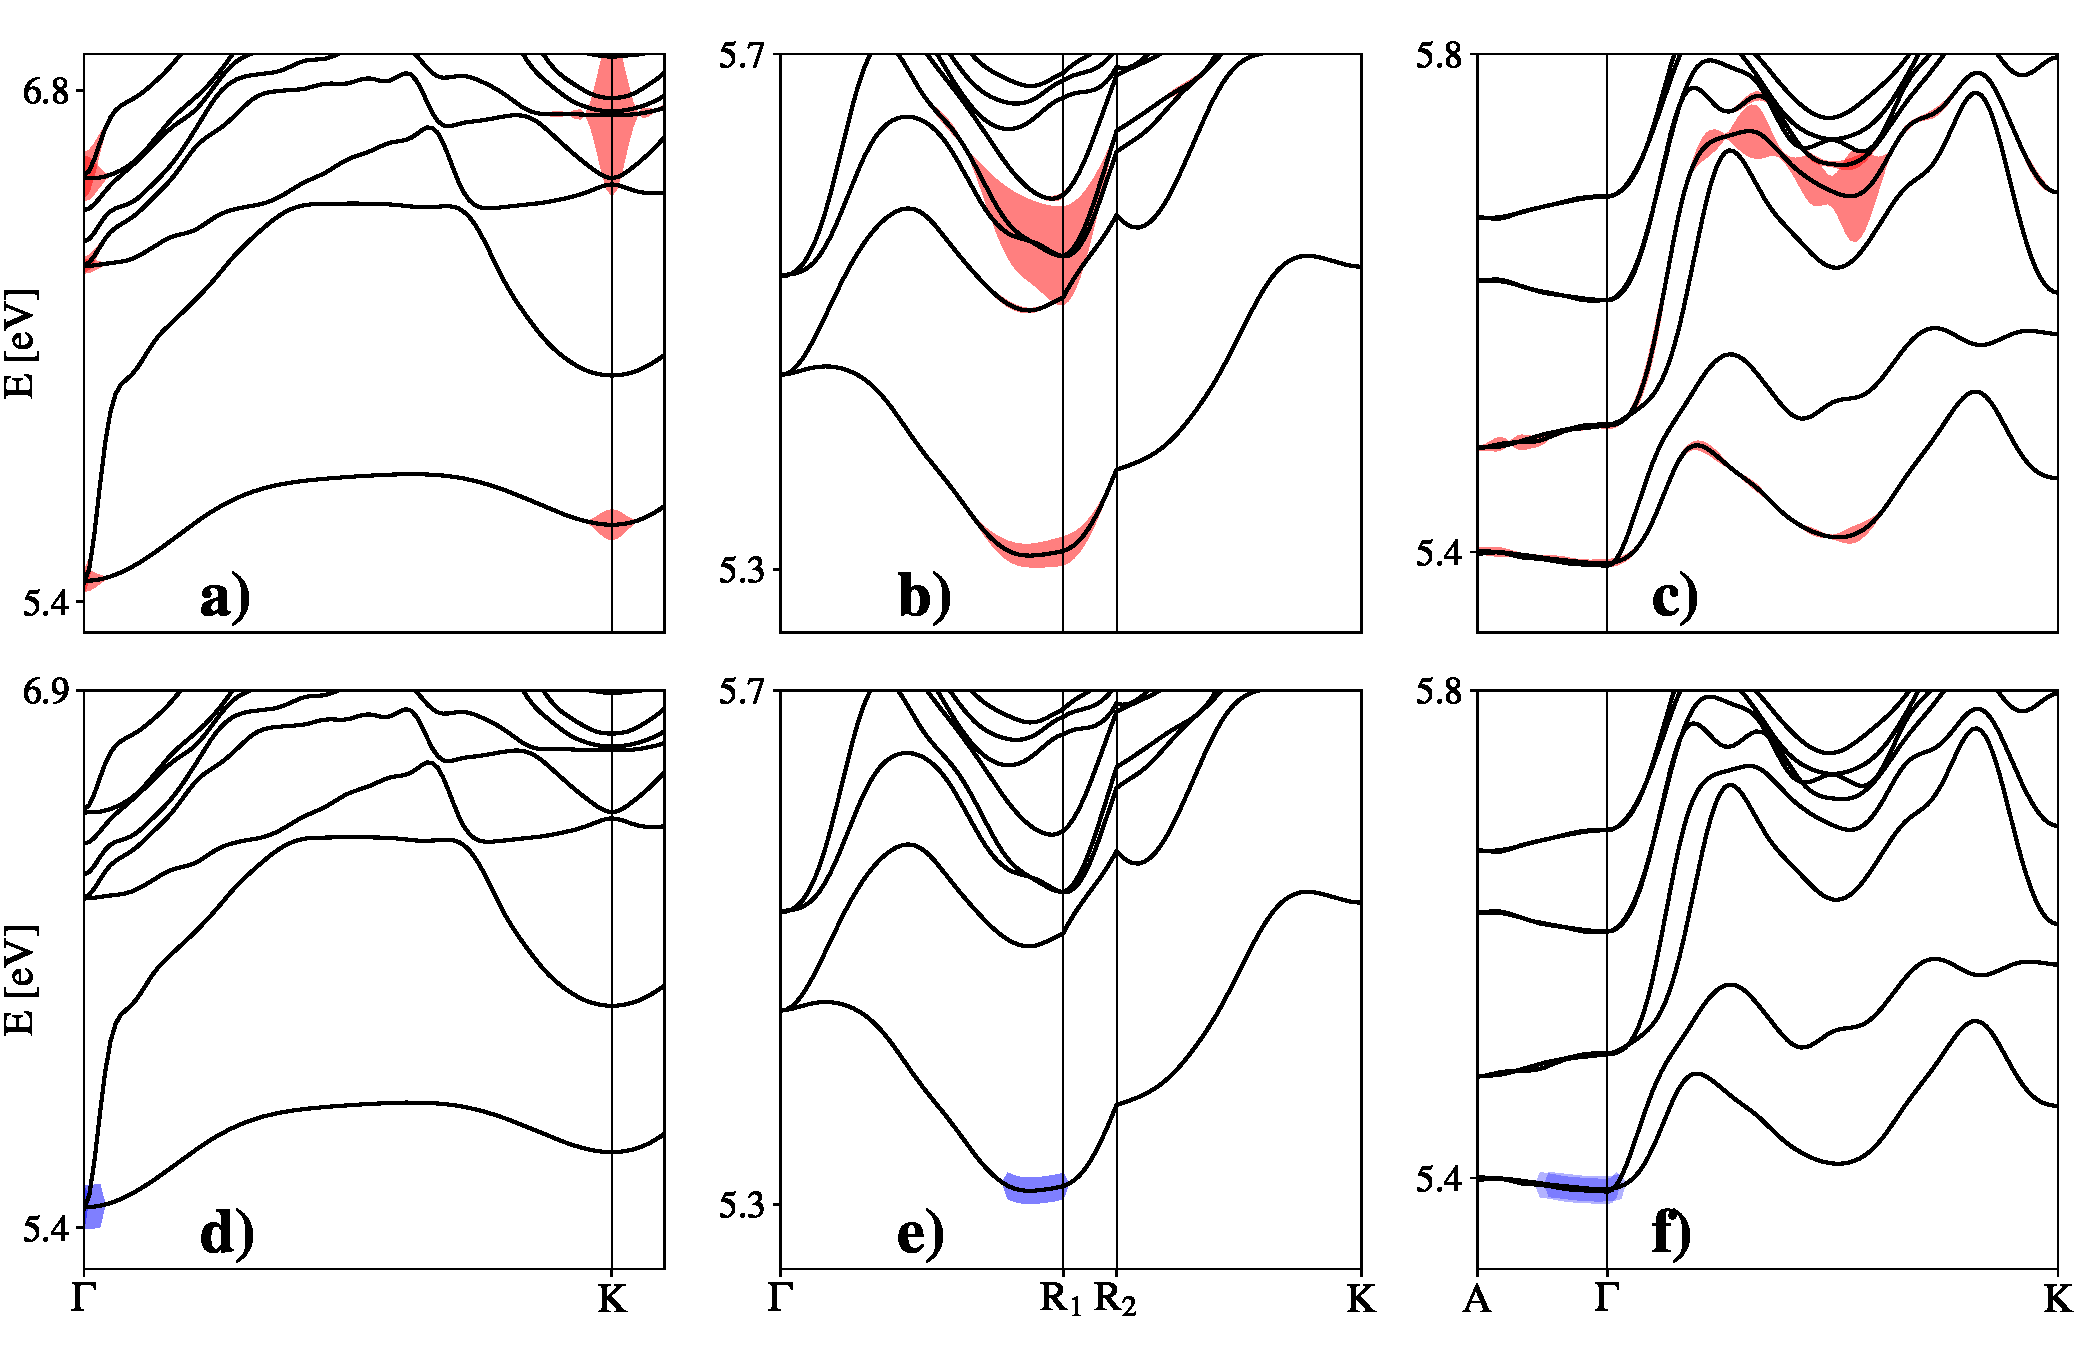
\includegraphics[width=0.9\textwidth]{all_occupations.pdf}
	\caption{Comparison of Boltzmann (blue areas) and quasi-Fermi (red areas) excitonic occupations for \acrshort{mBN} (first column), \acrshort{hBN} (second column) and bBN (third column). See main text for the definition of the occupation functions and section \ref{sec:bulk_hBN} for the definition of the R$_1$ and R$_2$ points. The black lines are the Fourier interpolation of exciton dispersions, calculated at the G$_0$W$_0$+BSE level. \textcolor{blue}{Add a BZ w/ R1 \& R2, labels to distinguish the 3 materials.}}
	%MODIF Add a BZ w/ R1 \& R2, labels to distinguish the 3 materials.
	\label{fig:all_occup}
\end{figure}

The final expression for luminescence intensity Eq. \eqref{eq:I_PL} is to be compared with the one obtained with the finite difference method in Chapter 2, Eq. \eqref{eq:strain_vRS_PL}. Unlike the previous method where only the indirect transitions were included, in the present formula we have both the term coming from direct transitions and the term related to phonon satellites. The major theoretical advance here is that the renormalization factor from Eq. \eqref{eq:renorm_fact} allows to compare the relative intensities of the direct and the satellite peaks. Besides, the satellite weight denominators include the addition or removal of the phonon frequency not present in the static approximation of Eq. \eqref{eq:strain_vRS_PL}. Finally, thanks to this \textit{ab initio} formulation we can perform the whole workflow necessary to evaluate Eq. \eqref{eq:I_PL} in the unit cell, which is also an improvement with respect to the previous method. 


\section{Excitons in mBN and exciton-phonon coupling}
In this section we will apply the theoretical development presented in the two previous sections to the case of monolayer hBN. We will first present its electronic and excitonic properties then we will include phonons and their coupling with excitons.
%
\subsection{Excitonic properties of a monolayer of hexagonal Boron Nitride}
The electronic and optical properties of \acrlong{mBN} have been the subject of numerous studies using both \emph{ab initio} and semi-empirical methods.\cite{galvani2016excitons}
Within DFT, with the LDA exchange-correlation functionals, \acrshort{mBN} is a direct band gap material at high-symmetry point $K$, but the G$_0$W$_0$ corrections change its gap from direct to indirect, going from $K$ to $\Gamma$.\cite{prete2020giant} 
We verified that the system remains indirect even at the semi-self-consistent ``eigenvalue-GW'' level (ev$GW$). We plot the electronic band structure in Fig. \ref{fig:mBN_bands_LDA_G0W0_G4W4} at different levels of theory : \acrshort{DFT} within the \acrshort{LDA}, G$_0$W$_0$ and evG$_4$W$_4$. The latter means that we iterated the Hedin's equation in the $GW$ approximation four times, modifying only the poles of $G$ at every iteration.\cite{van2006quasiparticle} This process is compensating the lack of higher order correction of the G$_0$W$_0$ approximation and usually improves the agreement with experiments regarding the bandgap values.\cite{faber2014excited}
\begin{figure}[h!b]
	\vspace{0.2cm}
	\setcapindent{2em}
	\centering
	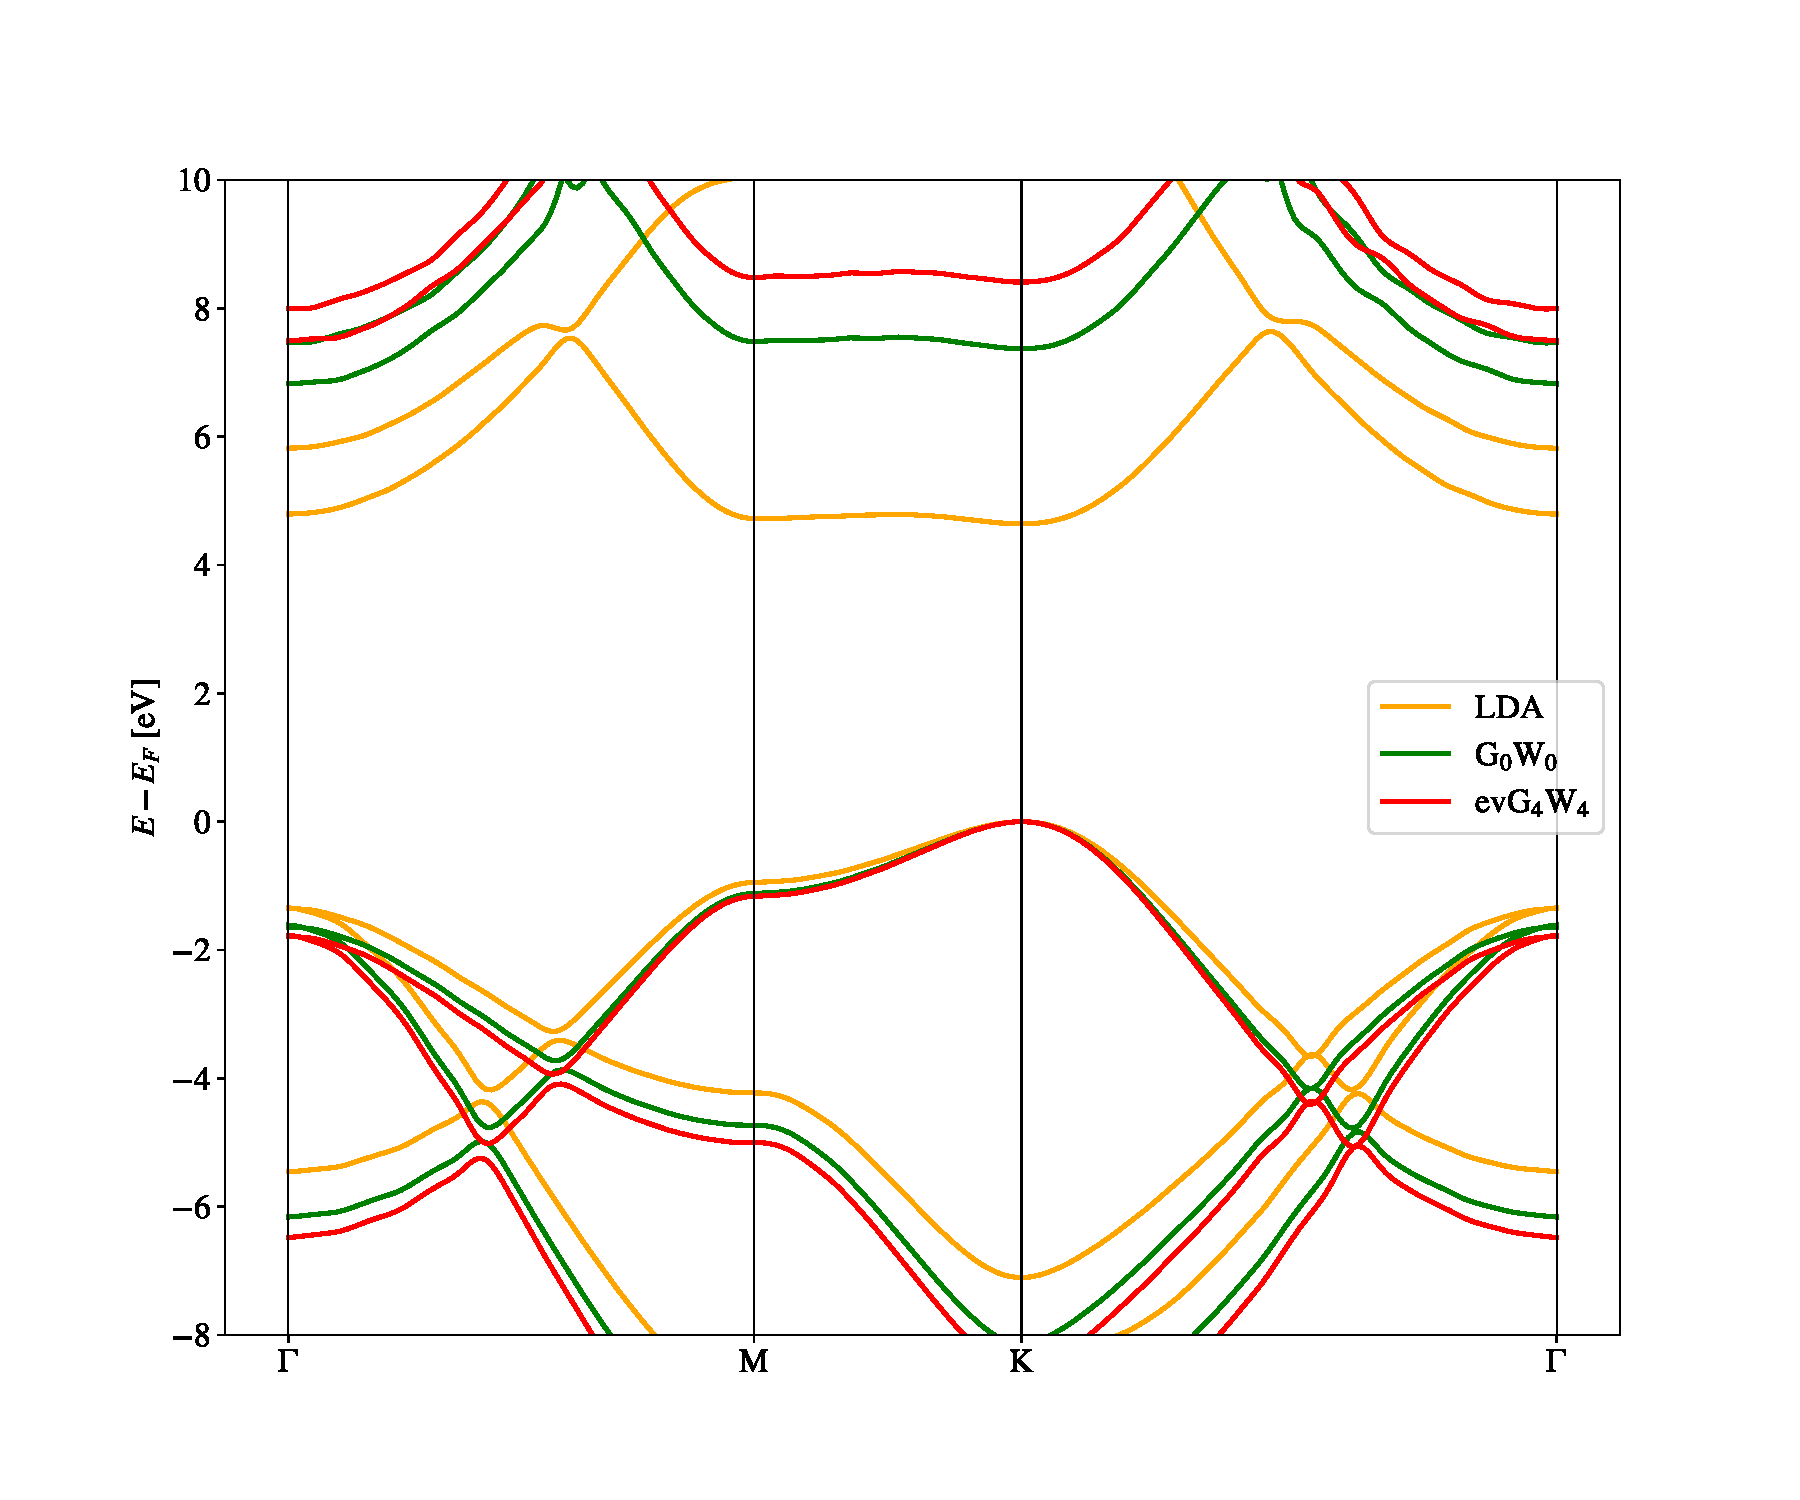
\includegraphics[width=0.8\textwidth]{mBN_bands_LDA_G0W0_G4W4.pdf}
	\caption{Electronic bands of freestanding monolayer BN with different levels of theory : DFT (orange), G$_ 0$W$_0$ (green) and evG$_4$W$_4$ (red)} %MODIF : bigger labels and ticks and legends % add \pi \pi* \sigma \sigma* annotations like in \cite{paleari2018excitons}
	\label{fig:mBN_bands_LDA_G0W0_G4W4}
\end{figure}
In \acrshort{mBN} the indirect gap is due to the presence of nearly-free electron states at $\Gamma$. 
In fact, the $GW$ self-energy does not correct the $\sigma^*$-like states at $\Gamma$ as much as the $\pi$-like states around $K$ and $M$ and this makes the system indirect.
The nearly-free electron states have been investigated in the past in BN nanotubes and mBN,\cite{blase1994stability,Blase1995monolayer} but only at the independent-particles, \acrshort{DFT} level. They may provide a possible mechanism for luminescence quenching.\cite{schue2016dimensionality}

Despite the presence of these states at $\Gamma$, the optical properties of BN-based systems are actually dictated by the $\pi$ bands around $K$ and $M$, and this remains true for mBN.
The optical spectrum of mBN is characterized by a strong doubly degenerate excitonic peak of symmetry $E$ at about $6$ eV. Exciton dispersions have been reported in several articles.\cite{cudazzo2016exciton,koskelo2017excitons,sponza2018direct} In Fig. \ref{fig:mBN_excdisp_lda_gw} we also report our calculated dispersion along selected high-symmetry lines, starting both from the quasiparticle band structure and the DFT one plus a scissor operator. The scissor shift is chosen in such a way that the lowest exciton energy at $\QQ = 0$ matches the one obtained starting from the $GW$ quasiparticle band structure. Our exciton dispersion compares well with previously publicated results.\cite{koskelo2017excitons,sponza2018direct}

\begin{figure}[h!b]
	\vspace{0.2cm}
	\setcapindent{2em}
	\centering
	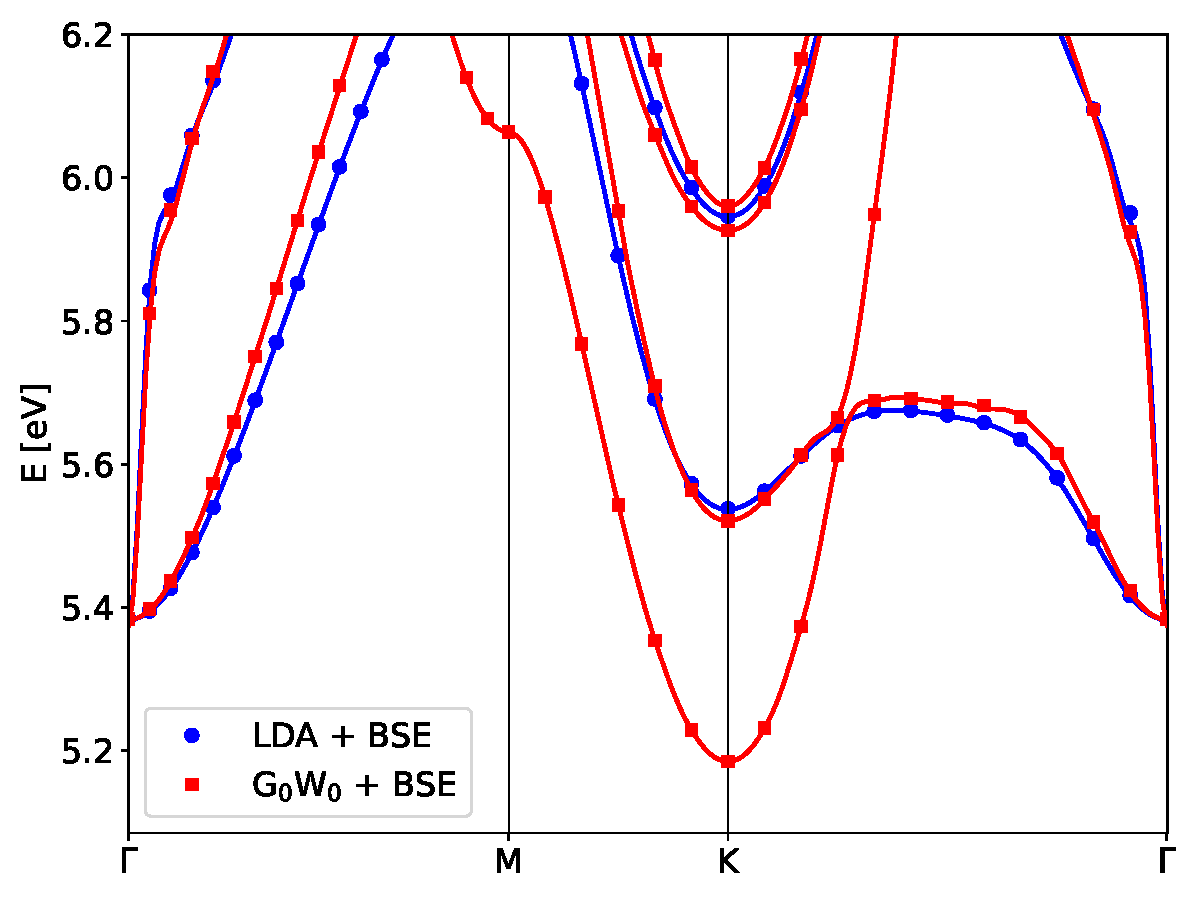
\includegraphics[width=0.8\textwidth]{mBN_excdisp_lda_gw.pdf}
	\caption{Calculated exciton dispersion for monolayer hBN, starting from either the DFT-LDA eigenvalues with a scissor operator (blue) or the G$_0$W$_0$ quasiparticle energies (red). Dots represent our calculated BSE data, lines are Fourier interpolations}
    %MODIF math font for labels, thicker lines and markers
	\label{fig:mBN_excdisp_lda_gw}
\end{figure}
We found that excitons at momentum $\qq=K$ have a lower energy than the direct exciton at $\qq=0$ when starting from the $G_0W_0$, a feature inherited from the indirectness of the quasiparticle structure. In fact, these low-energy excitons are due to transitions towards the nearly-free electron states at $\Gamma$.
These new excitonic states are clearly distinguishable from the ``standard'' BN excitons by plotting their wavefunctions in real space, as it is done in the insets of Fig. \ref{fig:mBN_excdisp_wf} for several different center-of-mass momenta of the various states. We plot the electron distribution in real space when fixing the hole just above a Nitrogen atom, like it would be in a $p_z$ orbital. This is what we call the exciton wavefunction in real space.

We tracked the exciton wavefunction of the lowest two bands the high-symmetry lines. We can see that the exciton momentum confers the wavefunction a shape according to the symmetry of the point, \textit{e.g.} it has a straight shape at \MM~but is circular at $\Gamma$ and \KK. 
While the usual $\pi \rightarrow \pi^*$-derived states (green exciton bands in the figure) display the electronic density strongly localized on the Boron sublattice, when the hole is fixed on top of a Nitrogen, the $\pi \rightarrow \sigma^*$-derived states (red exciton band) present an electron density strongly delocalized away from the layer plane. This is a clear signature of nearly-free electron character.
\begin{figure}[h!b]
	\vspace{0.2cm}
	\setcapindent{2em}
	\centering
	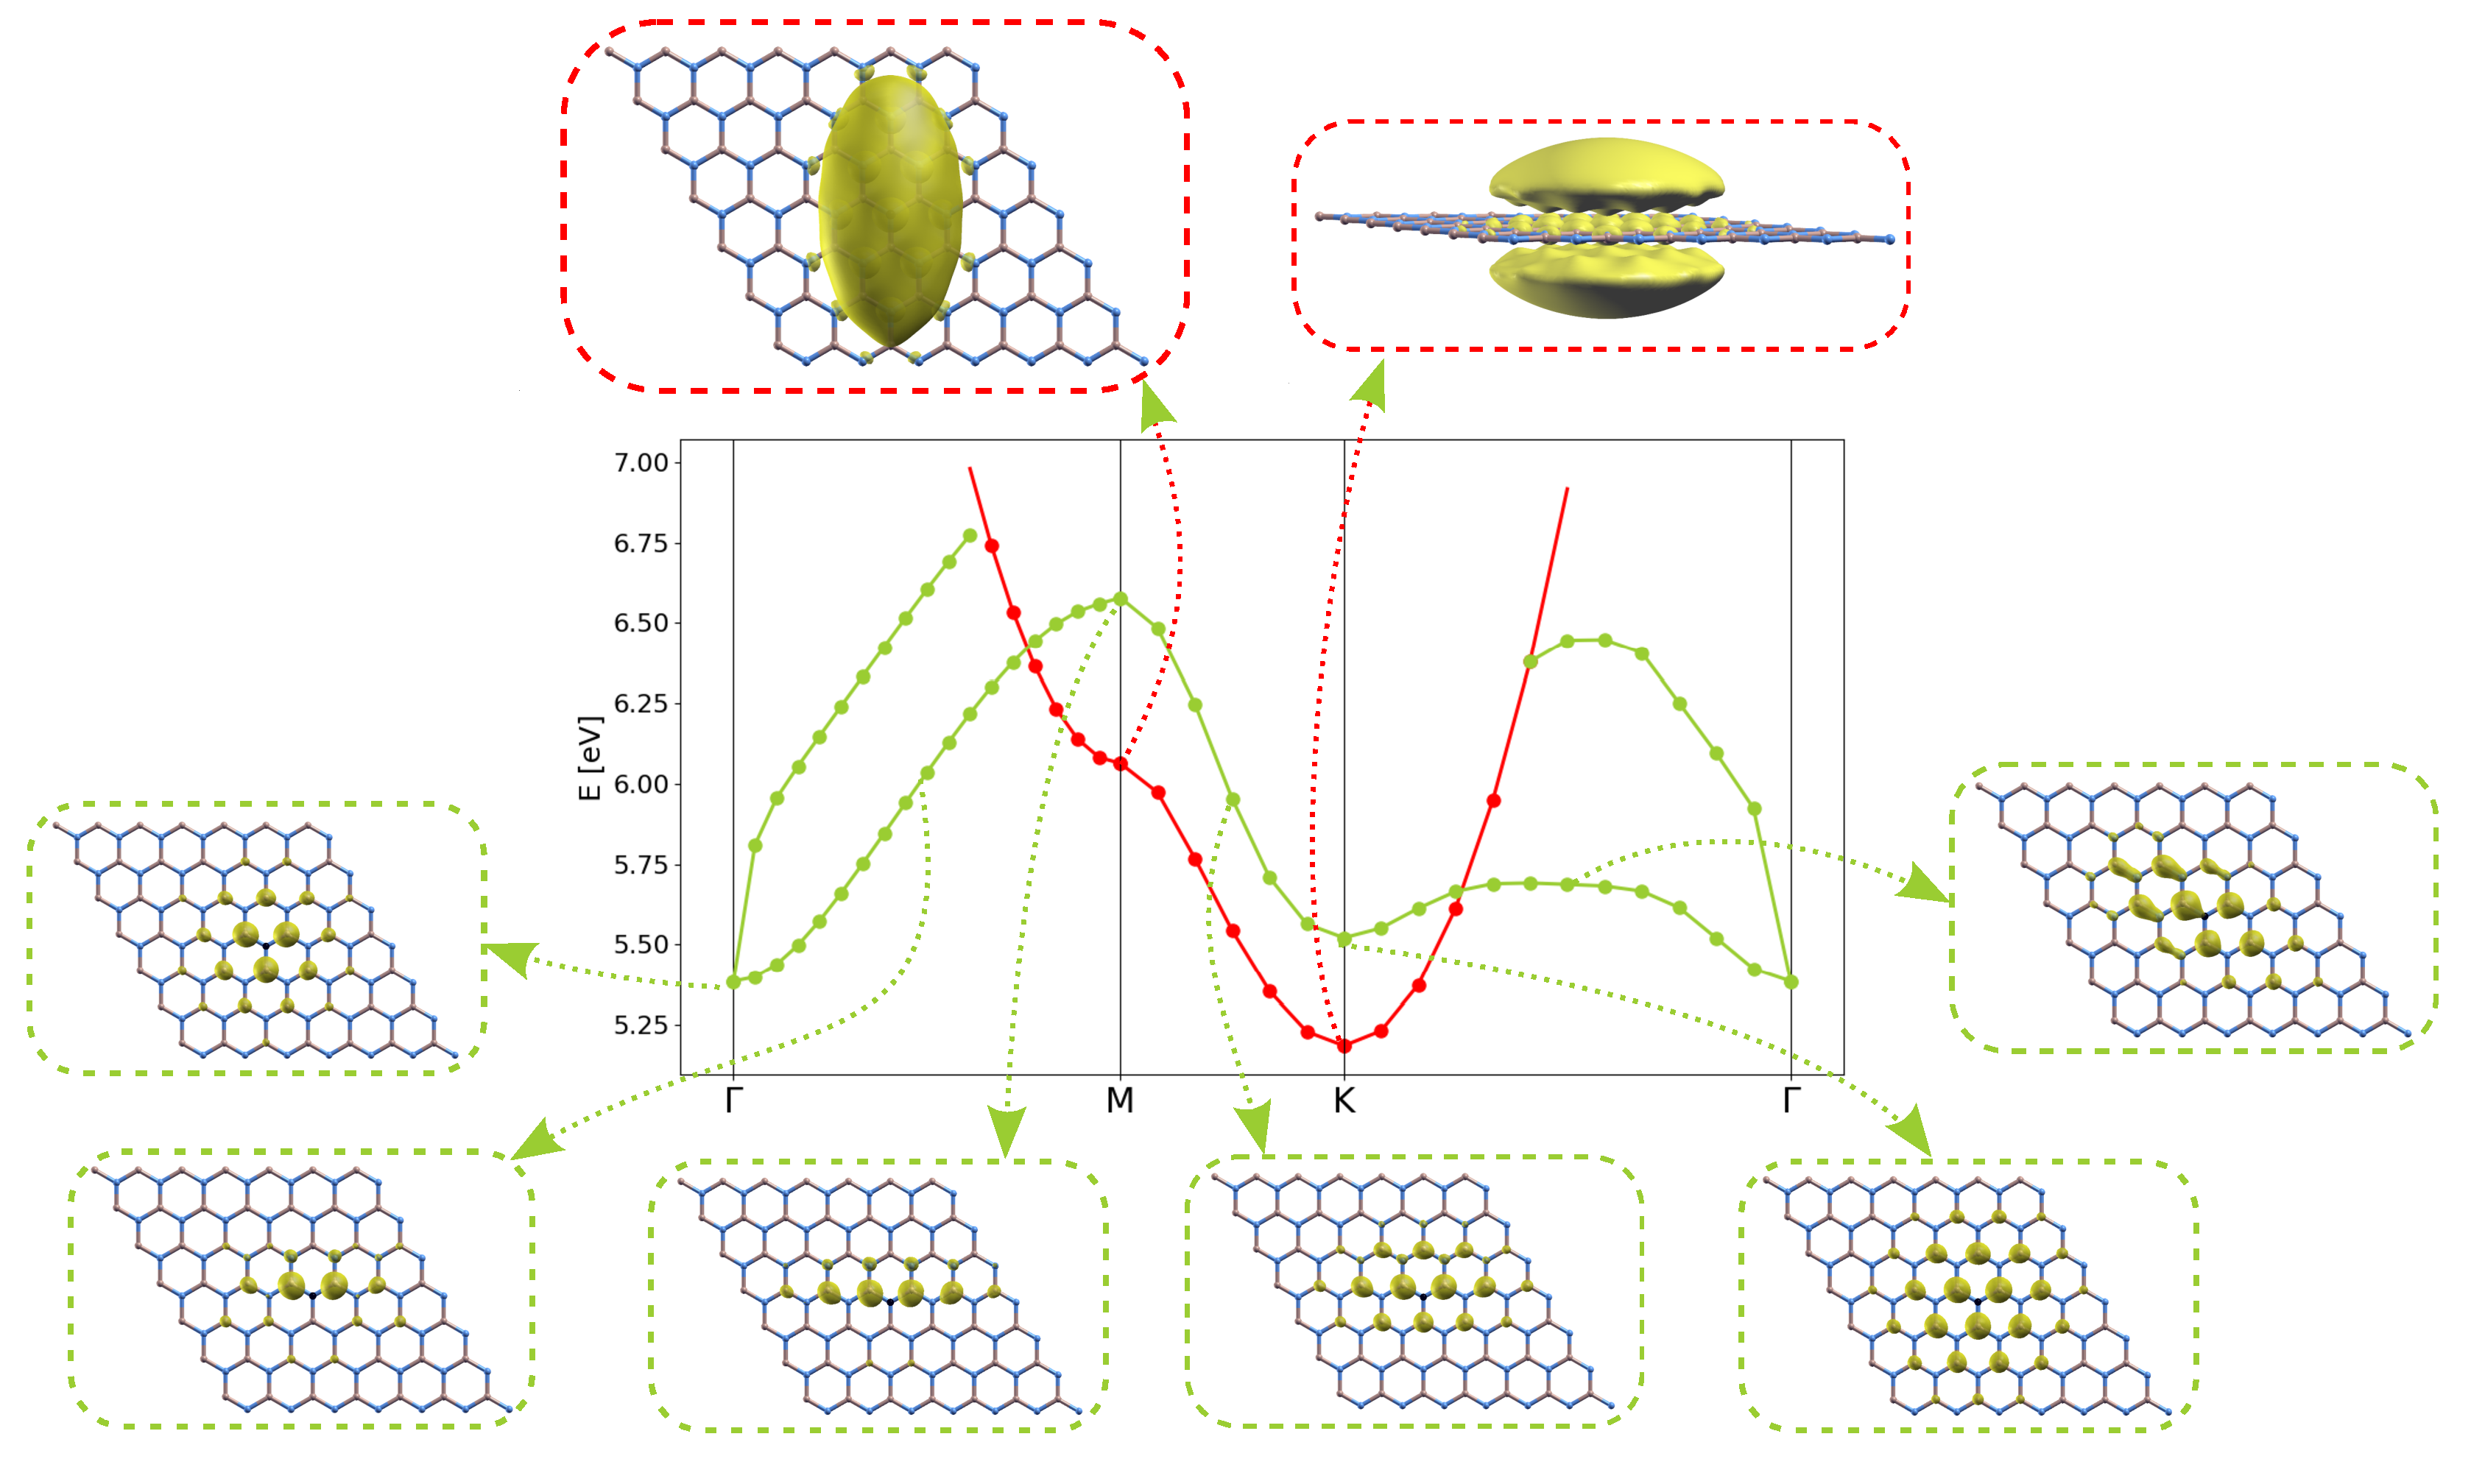
\includegraphics[width=0.95\textwidth]{1l_excdisp_disentangled.pdf}
	\caption{Details of the exciton dispersion of monolayer hexagonal BN. The insets show the spatial localization of the exciton wavefunction at several different $q$-points and branches (this is obtained by fixing the hole position on top of a Nitrogen atom, i.e. on a valence $\pi$ orbital, and plotting the resulting electron density). As evidenced in the insets, the red branch in the dispersion plot is due to the nearly-free electron states (involving conduction bands with $\sigma^*$ character), while the green branches originate from the optically active $\pi-\pi^*$ band transitions.}
	%MODIF : red arrows, bigger labels
	\label{fig:mBN_excdisp_wf}
\end{figure}

With this analysis and for other reasons that will be explained in Sec. \ref{sec:substrate}, we decided to use the \acrshort{DFT} eigenvalues with a scissor operator as a starting point of the \acrshort{BSE} and the subsequent steps, namely the calculation of exciton-phonon coupling and the luminescence spectrum.

%
\subsection{Exciton-phonon matrix elements resolved in momentum}
We can plot the calculated matrix elements over the \acrlong{BZ} thanks to the $\qq$-dependence in Eq. \eqref{eq:Gkkp}. 

\subsubsection{3D bulk hBN}
For the bulk hBN, we plot in Fig. \ref{fig:Gkkp_plot_hBN} the exciton-phonon coupling modulus for the lowest-lying finite-momentum excitons $\beta=1$ and $\beta=2$ scattered into the bright excitons $\lambda=3$ and $\lambda=4$ for all phonon modes. We sum over degenerate excitons and phonon modes. We average over the $\qq_z$ points belonging to discrete planes orthogonal to the $\Gamma A$ line in order to have a two-dimensional plot. The quantity we plot is : 
\begin{equation}
    |\mathcal{G}_{3+4,1+2}(\qq_\parallel)| = \frac{1}{N_{q_z}}\left|\sum_{\mu,q_z} \mathcal{G}^\mu_{3+4,1+2}(q_z,\qq_\parallel)\right|
\end{equation}
We also plot the same quantity but keeping only ZA and ZO phonon modes in the sum. 
\begin{figure}[h!t]%
	\vspace{0.2cm}
	\setcapindent{2em}
	\centering
    \subfloat[All phonon modes.]{\label{Gkkp_plot_hBN:all_phonons} 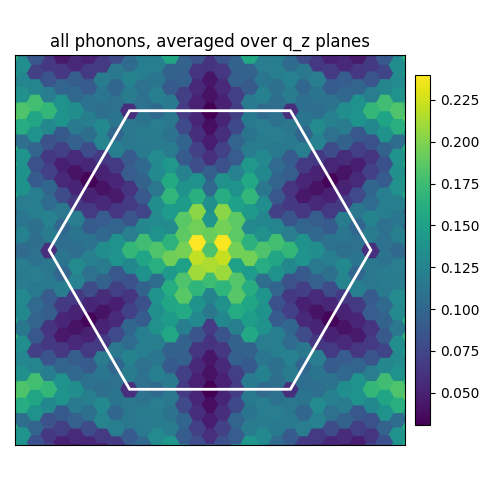
\includegraphics[width=0.45\textwidth]{hBN_all_phonons_all_planes.png}} \qquad 
    \subfloat[ZA+ZO modes only.]{\label{Gkkp_plot_hBN:z_only} 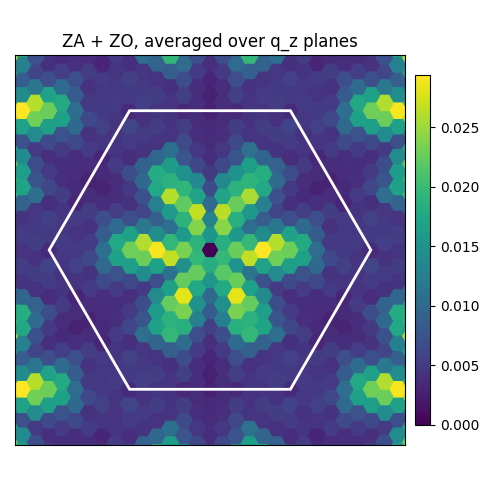
\includegraphics[width=0.45\textwidth]{hBN_z_only_all_planes.png}}%
    \caption{Magnitude of the coupling between the finite-momentum excitons and the lowest-lying bright excitons in bulk hexagonal BN. Color bar is the modulus of $\mathcal{G}(\qq)$ in eV, for a 18$\times$18 $\qq$-points grid. \textcolor{blue}{add label for colorbar}}
	\label{fig:Gkkp_plot_hBN}
\end{figure}
It is the probability that the excitons $\beta=1$ and $\beta=2$ are scattered into the zero-momentum excitons $\lambda=3$ and $\lambda=4$ by all phonon modes with the corresponding momentum. The information we can extract from this plot is that the coupling has the same symmetry as the crystal, where the 3-fold rotation symmetry is clearly visible. From the panel (a) of Fig. \ref{fig:Gkkp_plot_hBN}, we see that the scattering is maximal with excitons close to the $\Gamma A$ line. From the panel (b), we see that the ZA and ZO modes couple more with the minimum excitons on the $\Gamma K$ lines. This coupling contributes to about ten percent of the sum of all modes, as can be seen with the color bars.  

\subsubsection{2D mBN}
For the monolayer BN, we plot a similar quantity in Fig. \ref{fig:mBN_Gkkp}, except there is no need of averaging over planes since the \acrshort{BZ} is two-dimensional. We plot the scattering of finite-momentum excitons $\beta=1$ and $\beta=2$ into the two degenerate bright excitons $\lambda = 1$ and $\lambda = 2$ at $\Gamma$ (where the $\beta$ and $\lambda$ indices coincide).
\begin{figure}[h!t]
	\vspace{0.2cm}
	\setcapindent{2em}
	\centering
	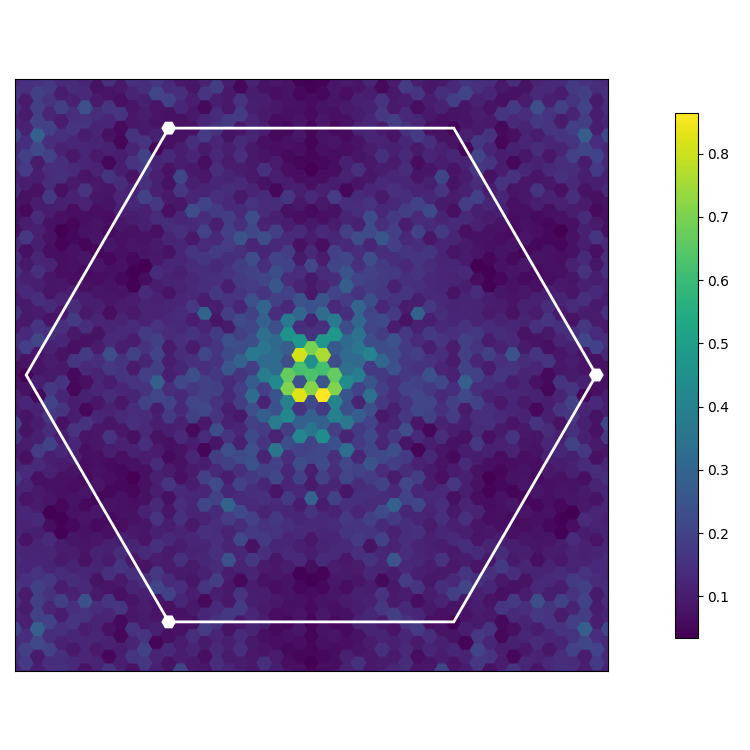
\includegraphics[width=0.55\textwidth]{mBN_Gkkp.png}
	\caption{Magnitude of the coupling between the finite-momentum excitons and the lowest-lying bright excitons in monolayer hBN. Color bar is the modulus of $\mathcal{G}(\qq)$ in eV for a $\qq$-points grid of 36$\times$36 grid. \textcolor{blue}{add label for colorbar}} 
	\label{fig:mBN_Gkkp} %MODIF : trim + add label
\end{figure}
Here the situation is different since most of the coupling happens around $\Gamma$ and is about 4 times stronger than in the bulk materials. The 3-fold hexagonal pattern can still be distinguished but with a lower coupling strength. This result is a first hint that in \acrshort{mBN}, it is less likely to see phonon-satellites coming from the scattering of an exciton at the \acrshort{BZ} edge than at the center.   


%
\section{Luminescence spectra}
%
\subsection{Benchmark on bulk hBN} \label{sec:bulk_hBN}
We now put to the test our method by calculating the luminescence spectra of bulk hBN which will serve as a benchmark. Indeed we can compare it to our finite difference method as well as existing calculations in the literature and most importantly to experiments. We plot in Fig. \ref{fig:ph_exc_disp_hBN} the phonon and exciton dispersion of bulk \acrlong{hBN}. The phonon dispersion has the labels of the different modes.
\begin{figure}[h!t]%
	\vspace{0.2cm}
	\setcapindent{2em}
	\centering
    \subfloat[Phonon dispersion of hBN]{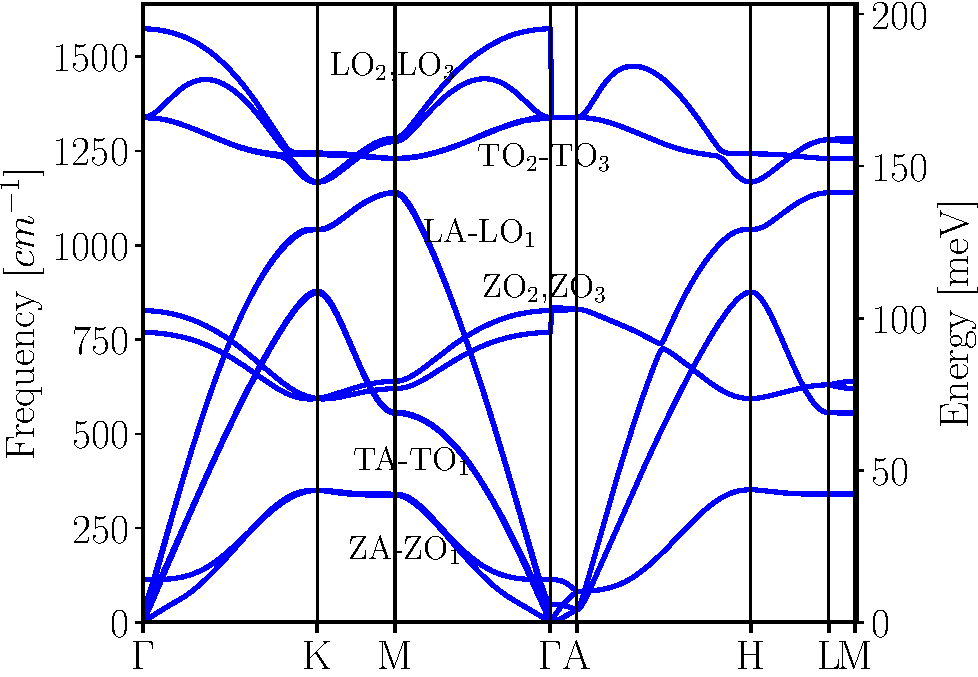
\includegraphics[width=0.42\textwidth]{hBN_phdisp.pdf}}
    \subfloat[Exciton dispersion of hBN \textcolor{blue}{ticklabel is wrong it is H instead of L}]{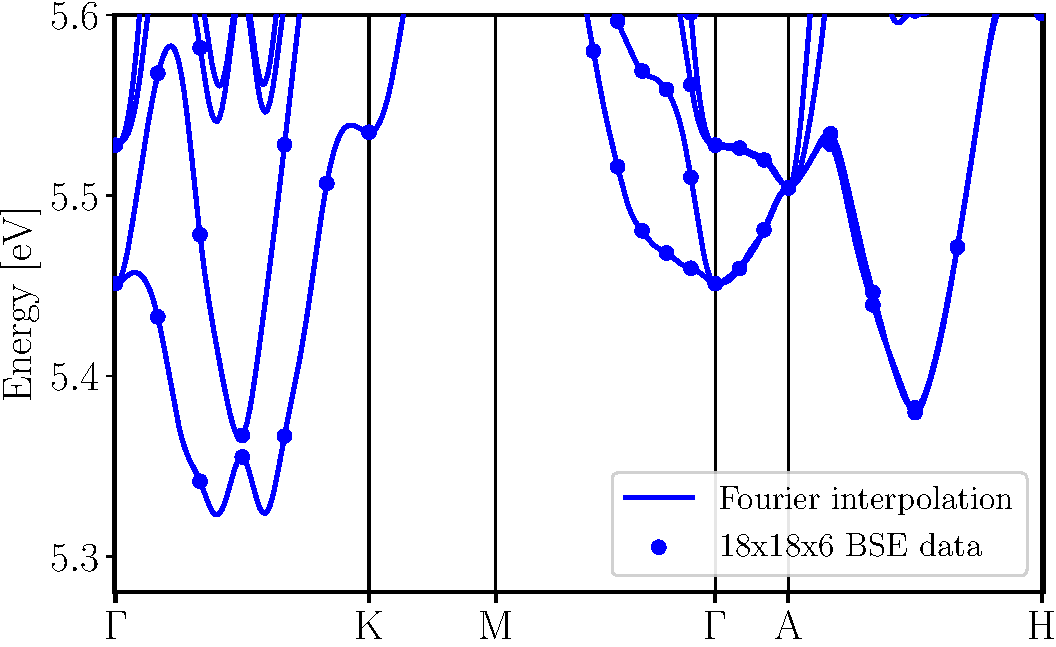
\includegraphics[width=0.48\textwidth]{hBN_excdisp.pdf}}
    \caption{Phonon (left) and exciton (right) dispersions of bulk \acrshort{hBN}.}
    \label{fig:ph_exc_disp_hBN} %MODIF : trim and same size for both
\end{figure}
The exciton dispersion exhibits a double local minimum on the $\Gamma K$ line with the Fourier interpolation. However the true minimum is on a point that is not on the $\Gamma K$ line. This is verified in Ref. \cite{zanfrognini2023distinguishing}.
With our coarse 18$\times$18$\times$6 momentum grid, the points with the minimum excitonic energies are labelled $R_1$ and $R_2$ and their reduced coordinates are fractions of the reciprocal lattice vectors $R_1=(\tfrac{1}{9},\tfrac{2}{9},0)$ and $R_2=(\tfrac{1}{9},\tfrac{5}{18},0)$. With the double-grid approach explained in Appendix \ref{app:comp_details_Chapt3}, the sampling of the exciton dispersion is much finer and the true minimum momentum is more accurately located.

In the left panel of Fig. \ref{fig:hBN_PL_comparison}, we plot the luminescence spectra obtained with the exciton-phonon coupling from finite difference, as presented in Chapter 2, compared with the present \textit{ab initio} method. The peaks are given by a Dirac delta function with a finite broadening added to follow a Lorentzian shape and match the experimental peak shapes (more numerical details can be found in Appendix \ref{app:comp_details_Chapt3}). The shape of the LA/TA phonon satellites on the high energy side of the spectrum, computed with the present \textit{ab initio} method, are broader than the single Lorentzian peaks of the finite difference method. This is a consequence of the integration on the full $\qq$-grid present in the former method and not in the latter. In addition, we used a double-grid for the exciton energies, the phonon frequencies but keeping the exciton-phonon matrix elements on the coarse grid, so that the numerical instabilities of the renormalization factor in Eq. \eqref{eq:renorm_fact} are smoothed out and the dispersions are accurately described. We verified that we obtain similar spectra when we restrict the sum on $\qq$ in Eq. \eqref{eq:I_PL} to the $\bar{q}$ points used in Chapter 2. The difference comes from the renormalization due to the denominators in the self-energy Eq. \eqref{eq:excph_SE_compact} which is missing in the finite difference formula. It should also be noted that the inclusion of phonon absorption processes does not give additional peaks in the spectrum. Indeed, the satellites due to phonon absorption have an intensity proportional to the Bose-Einstein occupation of phonons, which is low for the lattice temperature of 6 K we simulated. We have verified that these peaks appear when the lattice temperature is increased. Similarly, we have verified that higher-energy excitons become populated by the Boltzmann occupation function when we increased $T_{exc}$ and produce satellite peaks in the spectrum. 
\begin{figure}[h!b]%
	\vspace{0.2cm}
	\setcapindent{2em}
	\centering
    \subfloat[Comparison of finite-difference and \textit{ab initio} methods.]{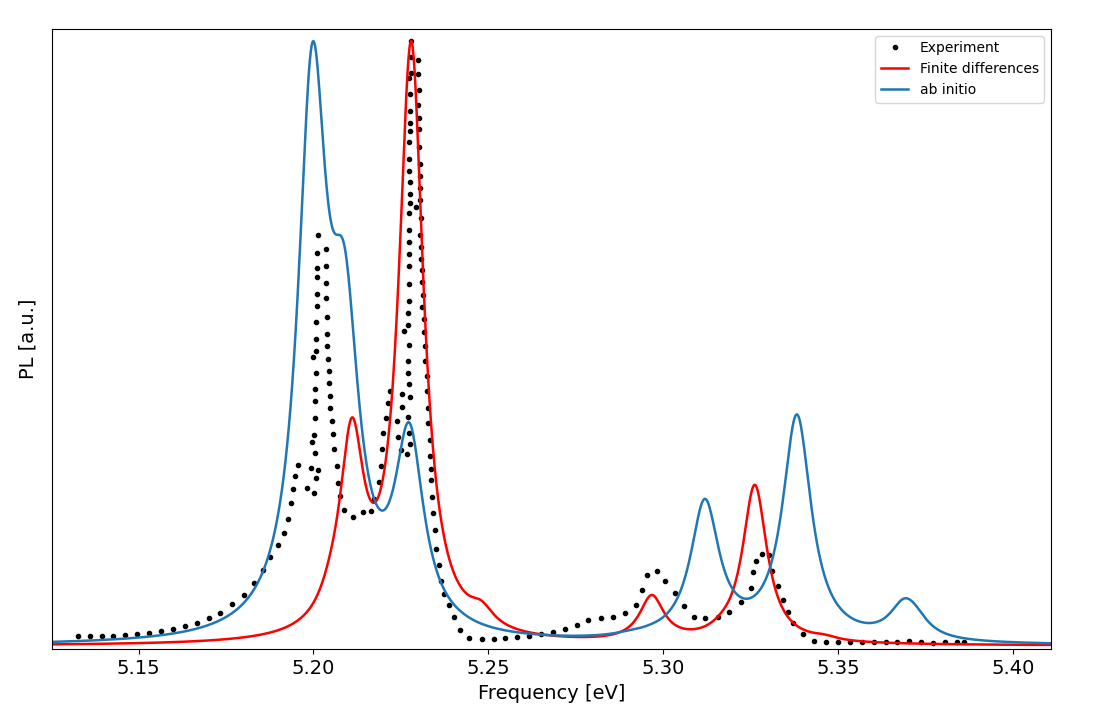
\includegraphics[width=0.45\textwidth]{comparison_pl.png}} \label{comparison_fdd} \qquad 
    \subfloat[Comparison of our \textit{ab initio} method and the one of Chen \textit{et al.}]{\label{comparison_ai} 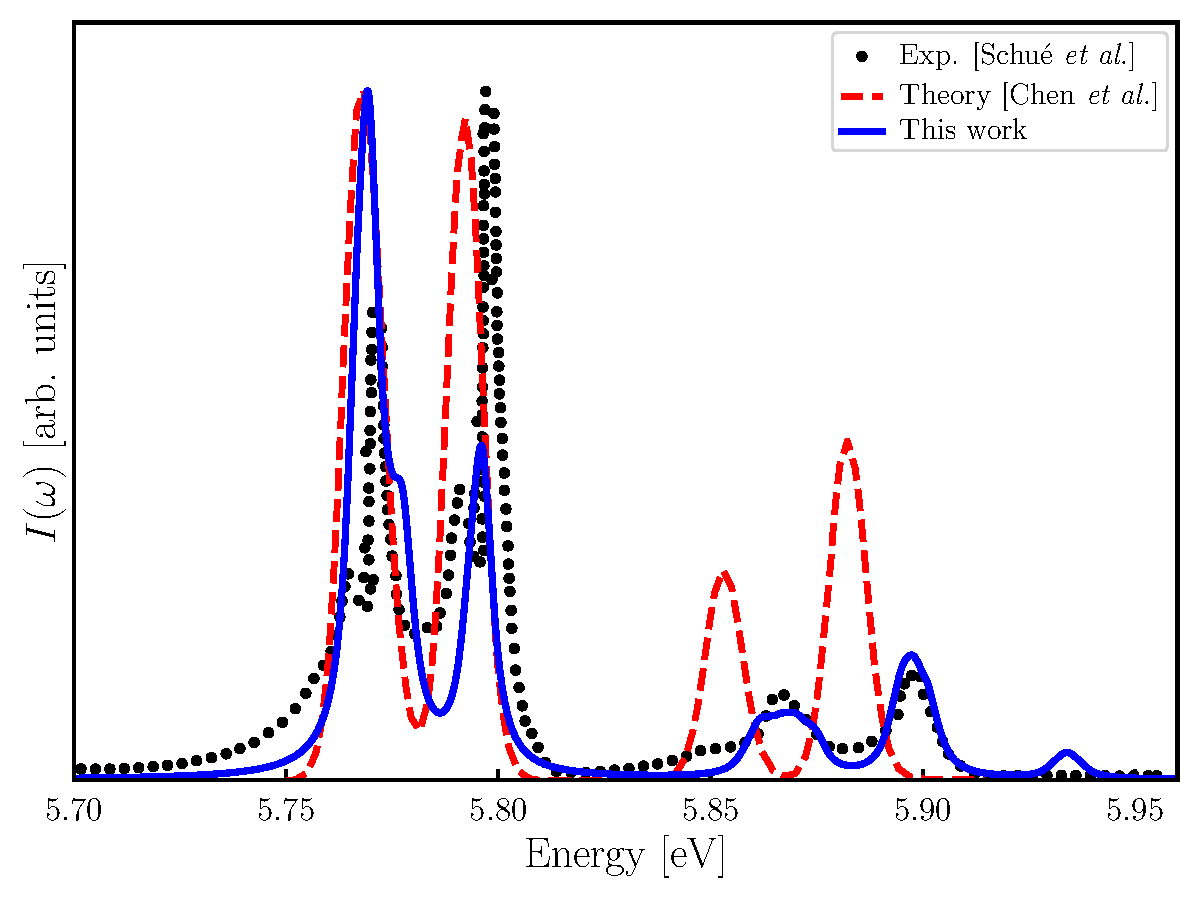
\includegraphics[width=0.45\textwidth]{hbn_pl_bulk.pdf}}%
    \caption{Comparisons of the normalized luminescence spectrum obtained with our \textit{ab initio} method (blue line) and the finite difference method (green line) on the left panel. On the right, we compare it to the result of Ref. \cite{chen2020exciton} (red dashed line). In both panels, the experimental data (black dots) comes from Ref. \cite{schue2019bright}.} %MODIF : trim and same size for both ; add labels for the peaks
	\label{fig:hBN_PL_comparison}
\end{figure}


In the right panel of Fig. \ref{fig:hBN_PL_comparison}, we also compare our result with the spectrum obtained by Chen \textit{et al.} in Ref. \cite{chen2020exciton}. As mentioned previously, the exciton-phonon matrix elements we compute are the same than in their formulation, if we do the correct change of variable to account for their different momentum conservation convention. We implemented their convention in \yambo~and verified that the spectra do not change when using one or the other. They compute the luminescence intensity differently than the van Roosbroeck--Shockley relation, this is why the spectra look different. Our spectrum reproduces correctly the position of the satellites measured in Ref. \cite{schue2019bright} (note that all spectra have been shifted to match the energy of the experimental peaks) and the intensity of the LA/TA doublet on the high energy side, which is an improvement compared to the results of Chen \textit{et al.}. However, the intensity of the LO/TO doublet on the low energy side is not well reproduced. It is in fact inverted, with the TO peak being less intense than the LO one. Since this inaccuracy in the intensity is still in the correct order of magnitude, we decided to proceed with this implementation. 

We can also notice that the experimental peaks have phonon overtones due to the scattering with multiple phonon which give them an asymmetric shape,\cite{vuong2017exciton} and this is not included in our framework.

Besides, another issue in the spectrum is the presence of a low intensity peak at 5.93 eV, which appear neither in other numerical spectra, nor in experimental measurements. To investigate the origin of this peak, we can separate the contribution of each phonon mode to the spectrum. We plot said contributions in Fig. \ref{fig:hBN_split_phonons}
\begin{figure}[h!t]%
	\vspace{0.1cm}
	\setcapindent{2em}
	\centering
    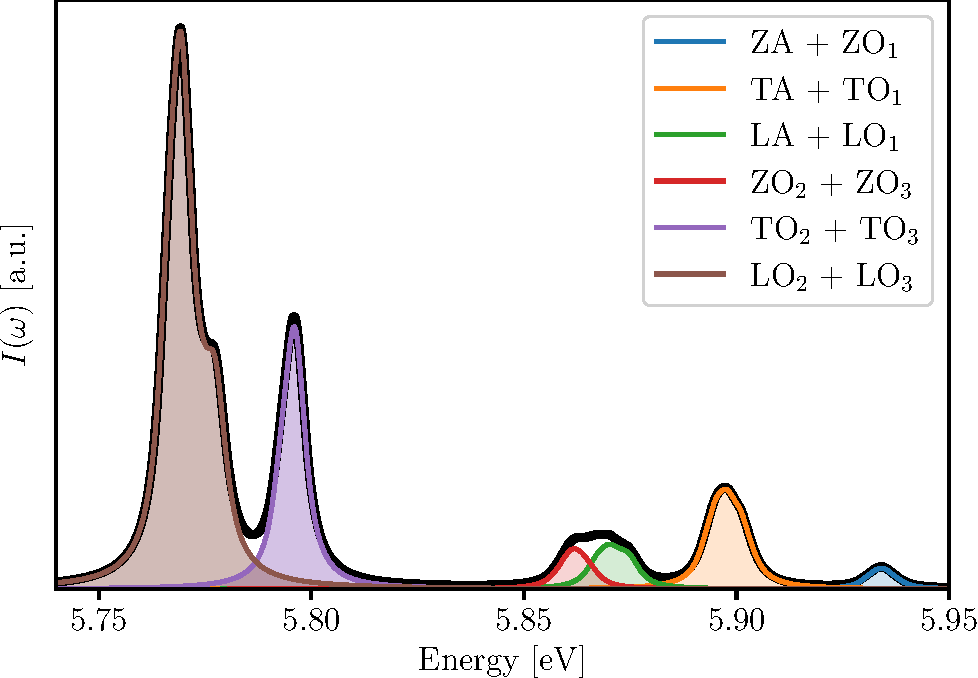
\includegraphics[width=0.6\textwidth]{hbn_pl_split_phonons.pdf}
    \caption{Luminescence spectrum of bulk hBN resolved with respect to the different
    phonon modes on the left panel and phonon dispersion on the right panel.}
	\label{fig:hBN_split_phonons}
\end{figure}
We see that the additional peaks come from scattering of excitons with ZO and ZA phonon modes. In our simulations, we set the light polarization to be in-plane. Hence optically created excitons are in-plane, and their scattering with out-of-plane phonons (namely the ZA and ZO modes) and their successive recombination is forbidden by symmetry.\cite{paleari2019exciton,cassabois2016hexagonal} If the crystal symmetries are changed, then these forbidden peaks can appear in photoluminescence. It is the case for rhombohedral BN.\cite{zanfrognini2023distinguishing} In our case, the problem arises from the construction of the exciton-phonon matrix elements in Eq. \eqref{eq:Gkkp}. The electron-phonon matrix elements and the exciton eigenvectors have different random phases that depend on the different sets of Kohn-Sham wavefunctions that were used to generate them in the first place. It is a non-trivial technical and numerical issue to account for these phases consistently.  Indeed, some \acrshort{DFPT} implementations (like \textsc{Quantum ESPRESSO}) recalculate the KS wavefunctions at $\kk+\qq$ for each $\qq$. Instead, a single set of wavefunctions is used to define the BSE matrix at any momentum $\QQ$ in the \yambo code, where the $\kk+\qq$ wavefunctions are obtained by symmetry transformations, thus imposing a specific choice of the relative phase between the wavefunctions. This difference causes a phase mismatch in the definition of the exciton-phonon matrix elements, Eq.~\eqref{eq:Gkkp}, because both the electron-phonon matrix element and the excitonic coefficients enter as full complex numbers. This is likely the reason why the magnitude of the coupling with ZA and ZO phonon modes is as large as displayed in Fig. \ref{fig:hBN_PL_comparison} (b).
This issue remains also if the electron-phonon matrix elements are obtained via Wannier interpolation\cite{chen2020exciton}, since the wavefunction used to construct the excitonic matrix would be different from the ones resulting via the Wannier procedure.\footnote{Notice the curve of Chen \textit{et al.} in panel (b) of Fig.\ref{fig:hBN_PL_comparison} ends at 5.9 eV, therefore we cannot compare the results for the ZA/ZO case.} In this case the interpolation process should be modified by fixing the wavefunction phases\cite{giustino2007electron}. 
The phase mismatch is not present in calculations based on finite differences\cite{paleari2018excitons,lechifflart2022excitons} because in this case exciton-phonon coupling is directly calculated as a derivative of the exciton dipole matrix elements on a supercell. However, these types of calculations are restricted to a single $\qq$-vector.
In the case of hBN luminescence, we verified that the phase mismatch only gives small changes in the numerical results (by testing different sets of wavefunctions with different random phases). 

A workaround of these issues was used by Zanfrognini \textit{et al.} in Ref. \cite{zanfrognini2023distinguishing} where the same implementation was used to compute the luminescence of bulk \acrshort{hBN} and rhombohedral BN. They did not use the crystal symmetries to reduce the size of the \acrshort{BZ} and wrote an interface with a third simulation code in order to build the exciton-phonon matrix elements without the phase issue. Overall, this was a much heavier numerical calculation but it allowed to solve two issues in the spectrum.
The spectrum they obtained for \acrshort{hBN} does not contain the ZA/ZO satellite and has improved relative intensities for the LO/TO and LA/TA doublet with respect to experiments.

Overall, our spectrum is in fairly good agreement with the experimental one. Keeping in mind the issues discussed above, we turn to the study of a case where the main advantage of our method is fully exploited : the fact that we can compare the relative intensities of direct peaks and phonon satellites.

%
\subsection{Results on mBN}
In this section we report the luminescence spectrum of monolayer hBN calculated using the method presented in Sec. \ref{sec:PL_ai} with the computational parameters reported in Appendix \ref{app:comp_details_Chapt3}. Here we consider an isolated monolayer and compared our results with different experiments reported in the literature. The effect of the substrate will be discussed in the next sections.
\begin{figure}[H]
	\vspace{0.2cm}
	\setcapindent{2em}
	\centering
	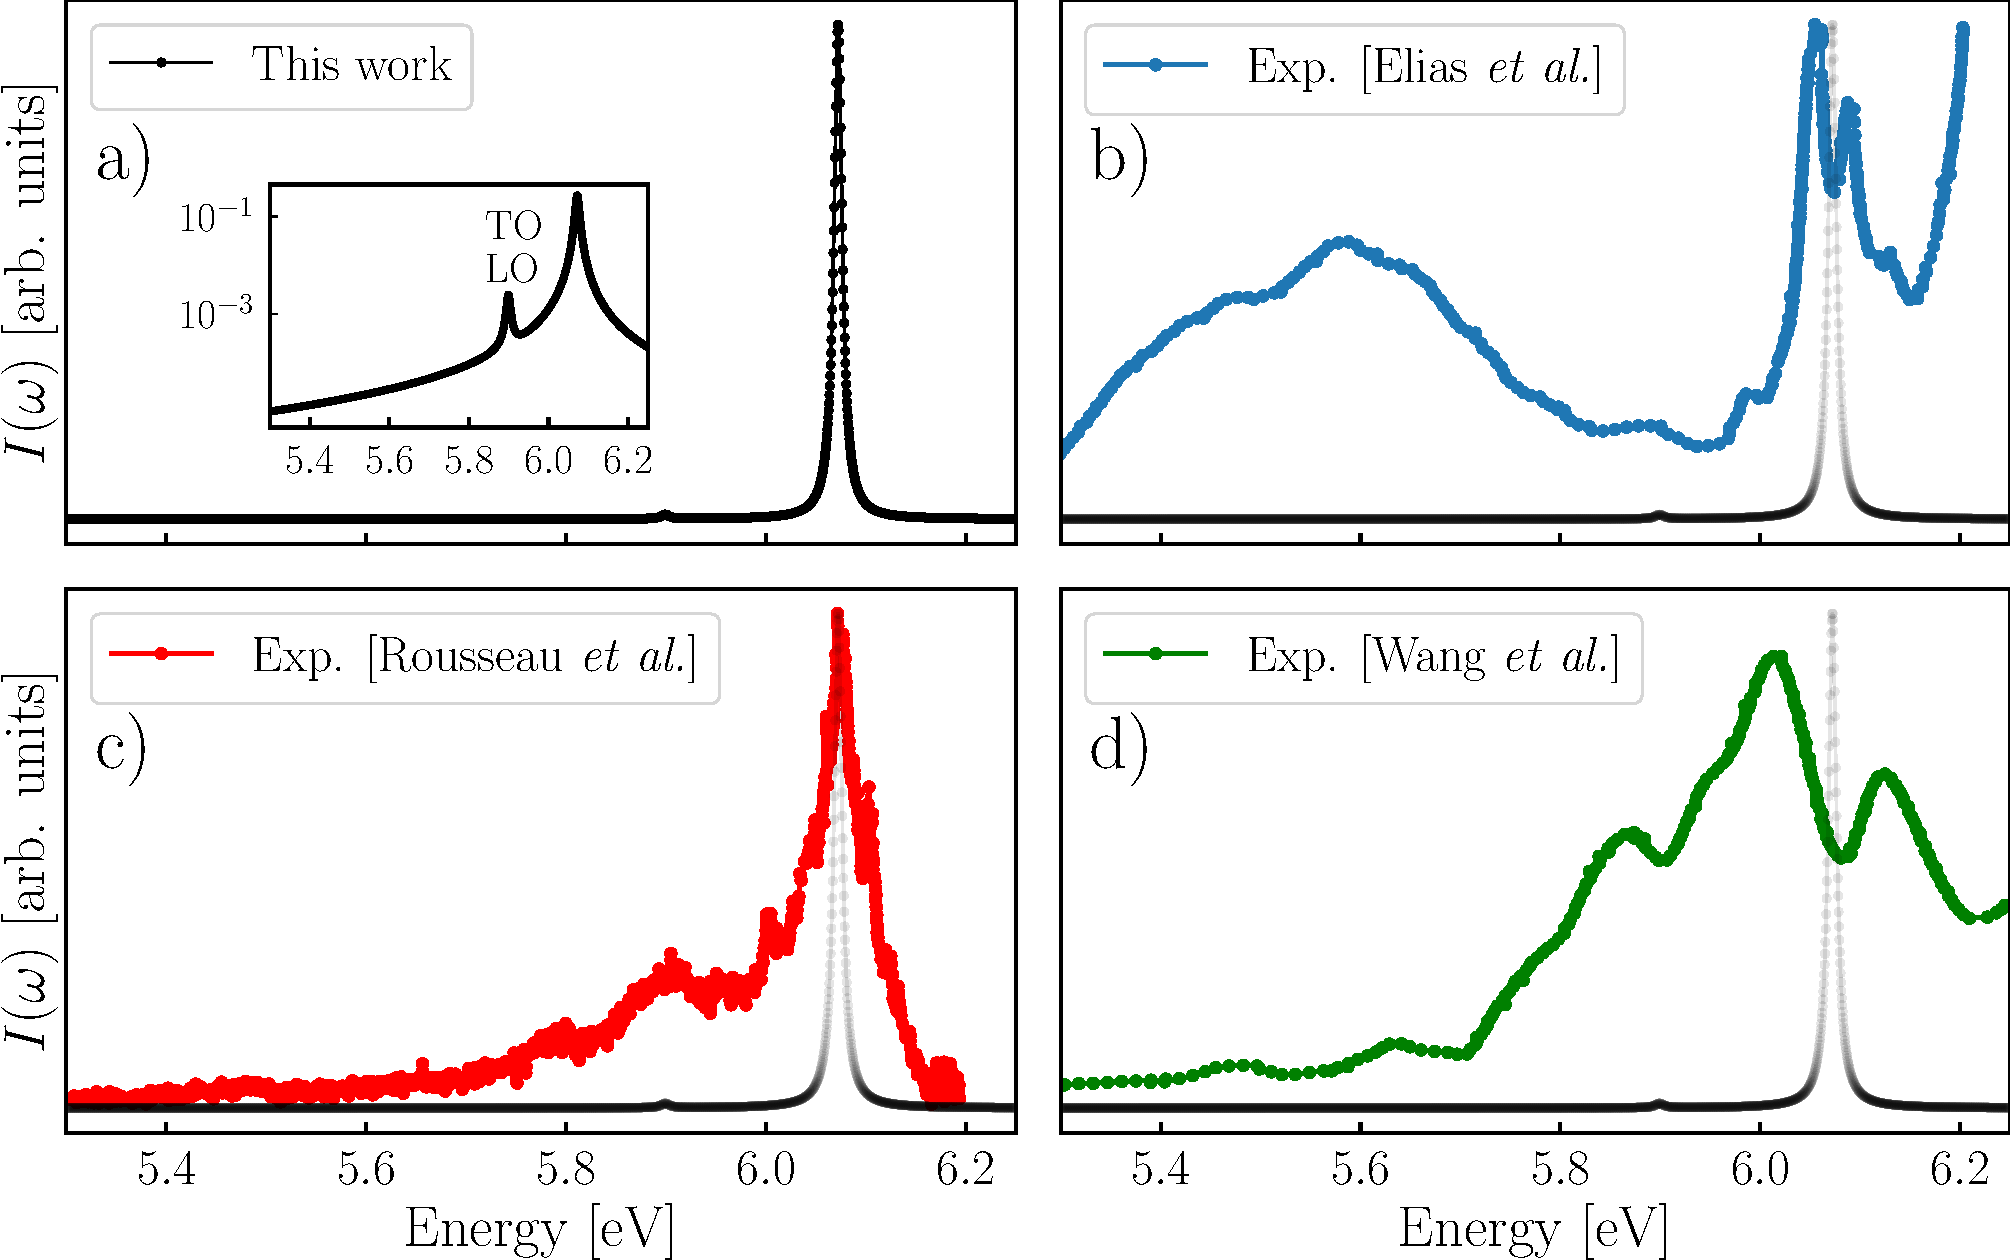
\includegraphics[width=0.9\textwidth]{hBN_monolayer_lum2.pdf}
	\caption{Calculated luminescence spectrum of monolayer hBN (a) compared to the experimental results of Ref. \cite{elias2019direct}(b), Ref. \cite{rousseau2021monolayer}(c) and Ref. \cite{wang2022scalable}(d). The theoretical spectrum has been shifted to match the main experimental peak (c). For clarity, we have plotted the theoretical spectrum next to each experimental result. In the inset of panel (a) we show the theoretical spectrum in a logarithmic scale, revealing the presence of a small phonon satellite.} 
	\label{fig:mBN_PL} %MODIF: put the scale for the log inset
\end{figure}
We plot the central result of this chapter in Fig. \ref{fig:mBN_PL}. In panel (a) we report our luminescence calculations of a single layer m-hBN compared to the measurements of Refs. \cite{elias2019direct,wang2022scalable,rousseau2021monolayer}, panels (b),(c),(d). Beside the main direct emission peak, we found a satellite at lower energy that has a small intensity, about two orders of magnitude lower than the direct peak (see inset in logarithmic scale in the panel (a)). We were able to identify the different terms contributing to the satellite intensity by analyzing the single terms of the sum in Eq. \eqref{eq:I_PL}, both in terms of phonons modes and in momenta. Thus we identify the satellite as a scattering from a zero-momentum exciton due to the LO and TO phonons.

 We also included possible indirect transition from excitons with momentum corresponding to the $K$ point due to the $\pi \rightarrow \pi^*$ transitions (relative minimum of the green curve in Fig. \ref{fig:mBN_excdisp_wf}). However, we found that due to the relatively large energy difference of $0.14$~eV between direct and indirect excitons, the contribution of these latter states to the luminescence spectrum is null.\footnote{We did not consider polaritonic effects that could slightly modify the luminescence spectra, see Ref. \cite{henriques2019optical} for a discussion.} Therefore, the additional peaks seen in some of the experiments are not explained by our calculations.

Finally as a sanity check, we considered the possibility that the distance between the exciton $\KK$ and $\Gamma$ is not well reproduced by our calculations and analyzed the matrix elements of the phonon-assisted transitions between $\KK$ and $\Gamma$. We found that these are in any case too small to explain the additional peak seen close to the main one in the experiments with a Graphite substrate.

In the light of these results, let us now discuss the different experiments. The details of the three luminescence spectra reported in the literature, see Fig.~\ref{fig:mBN_PL}(b-d), are the following: two of them feature mBN grown by molecular beam epitaxy on Graphite,\cite{elias2019direct,wang2022scalable} and one mechanically exfoliated on Silicon Oxide.\cite{rousseau2021monolayer}
With the Graphite substrate, multiple peaks are visible.
These peaks have been attributed to various causes, which we will briefly summarized here. In the work of Elias \emph{et al.},\cite{elias2019direct} the possibility of additional satellites appearing due to scattering of the indirect excitons at $K$ was considered. We also mention that in a very recent article, not peer-reviewed yet,\cite{shima2023cathodoluminescence} cathodoluminescence measurements of mBN on Graphite revealed a faint peak at 6.04 eV, that was attributed to the phonon-assisted recombination of the $K$ exciton assisted with a ZA phonon.
In the work of Rousseau \emph{et al.}\cite{rousseau2021monolayer} they put forward the possible presence of bubbles in the sample as cause of the additional peaks. 
Finally, in the article of Wang \emph{et al.}\cite{wang2022scalable}, these additional peaks were attributed to the presence of multilayer BN regions and the peak at the middle of the three should be caused by defects that would allow the triplet excitons (out of the scope of this thesis) to recombine radiatively. \\


Our theoretical work allows us to rule out the first hypothesis since, as shown above, the energy difference between $\Gamma$ and $\KK$ is large and the phonon-assisted transitions have too low an intensity to have indirect excitons visible in luminescence in the energy range where the second experimental peak appears, while the $\pi\rightarrow\sigma^*$ transitions seem to play no role. Regarding the effect of bubbles in the sample on the luminescence spectra, we have shown in the previous Chapter that strain can induce shifts of the luminescence spectra.\cite{lechifflart2022excitons}
Yet, in order to obtain a significant effect, the strain must be very large, and in addition it is difficult to explain with strain the presence of two well-defined peaks, like those visible in the experimental spectra. 
Finally, there is the hypothesis of defects or multi-layers BN. We think this is the most plausible hypothesis, because it has been shown that some defects can produce levels close to the main exciton,\cite{attaccalite2011coupling} and multi-layers BN induce splittings of the main peak.\cite{paleari2018excitons} 
Finally, note that the presence of defects or edges, which break translational symmetry, could make the indirect exciton visible without the need for phonon mediation.\cite{feierabend2017proposal}


%
\section{Effects of the substrate on the electronic bands and excitons of mBN} \label{sec:substrate}
In the previous section we considered the isolated \acrshort{mBN} and its luminescence spectrum. However it is well known that the interaction of 2D materials with a substrate can strongly modify their electronic and optical properties. In this section we analyze how the presence of a Graphite substrate could modify the picture presented in the previous section. In particular, we will investigate the role of nearly-free electron states and of indirect excitons.
In order to see if we can really expect an optical experimental signature from the exciton made of nearly-free electron states -- that will make the system functionally indirect -- we decided to investigate how the presence of a substrate modifies their position with respect to the direct gap, compared to the freestanding mBN. We included a graphitic substrate in the simulation, analogous to the one used in some of the experiments. Since we are not able to include a full bulk Graphite in the simulation, we modelled it with one and two layers of Graphene. We found that the presence of a graphitic substrate lowers the direct gap at $K$ much more than the indirect one, actually making the system a true direct band gap insulator again. This is most likely due to the stronger interaction of the $p_z$ orbitals of boron with those of Graphene while the planar $\sigma^*$ states are less affected. The dependence of the mBN gaps on the number of substrate Graphene layers is shown in Fig. \ref{fig:mBN_gap_layers} (calculation details are given in Appendix \ref{app:comp_details_Chapt3}). 
\begin{figure}[H]
	\vspace{0.2cm}
	\setcapindent{2em}
	\centering
	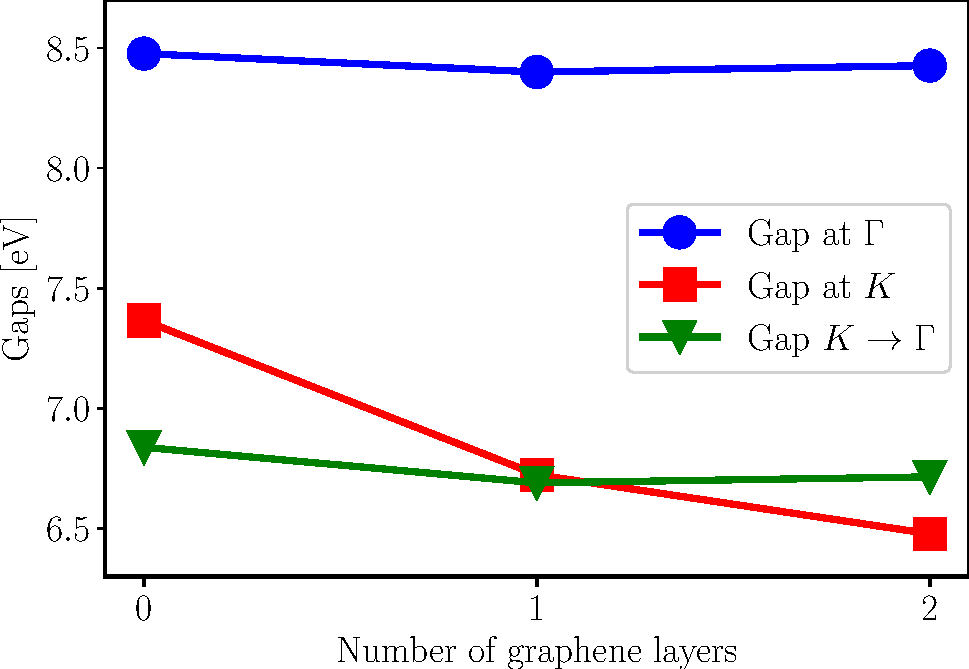
\includegraphics[width=0.8\textwidth]{mBN_gap_vs_layers.pdf}
	\caption{Band gaps of mBN as a function of the number of graphene layers\label{gap_vs_layers}. The large direct gap at $\Gamma$ is in blue, the indirect $\pi\rightarrow\sigma^*$, i.e. $K\rightarrow\Gamma$, is in green and the smallest $K\rightarrow K$ direct gap is in red.} %MODIF : légendes plus grosses, lignes et points plus gros (check my paper with Conor for inspiration) 
	\label{fig:mBN_gap_layers}
\end{figure}
Therefore, we expect that these states at $\Gamma$ will not contribute to the luminescence in a realistic experiment where mBN is deposited or grown on a substrate.
In order to simulate luminescence from an ideal mBN deposited on a substrate we started from the LDA band structure and applied a scissor operator that allows us to maintain the direct nature of mBN (\textit{i.e.} removing the red ``band'' in Fig. \ref{fig:mBN_excdisp_wf}).\\ 


Next, we investigate the effect of a substrate on the indirect excitons of \acrshort{mBN}. As computing the excitonic dispersion in the presence of a substrate would be computationally prohibitive, we decided to use a simple model to study the impact on luminescence. We know that the difference in energy between the excitons at $\Gamma$ and $K$ is due to correlation effects. Therefore with the substrate increasing the screening, we expect this gap to decrease.
Indeed, with increased screening the attractive term in the \acrshort{BSE} kernel is stronger, hence increasing the finite-momentum excitons binding energy. By adding a parameter that renormalizes the exciton energies proportionally to their momentum with the formula $E(\qq) = E_0(\qq) + \alpha |\qq|$, we can roughly simulate this effect and bring the exciton at $K$ lower in energy than the one at $\Gamma$. Hence, this new minimum gets more populated with the Boltzmann occupation function and it might increase the intensity of phonon satellites. An \textit{ab initio} treatment of the Graphite substrate is possible at the $GW$ and BSE level with recent numerical developments,\cite{guandalini2023efficient} but it remains too expansive computationally for our way of calculating the exciton-phonon coupling, given the number of $\kk$ and $\qq$ points needed to accurately describe the sharp electronic dispersion of Graphene layers. More advanced numerical procedures to include the screening of a substrate or any external environment exist,\cite{ugeda2014giant,bradley2015probing} but they are beyond the scope of this thesis.
\begin{figure}[H]
	\vspace{0.2cm}
	\setcapindent{2em}
	\centering
	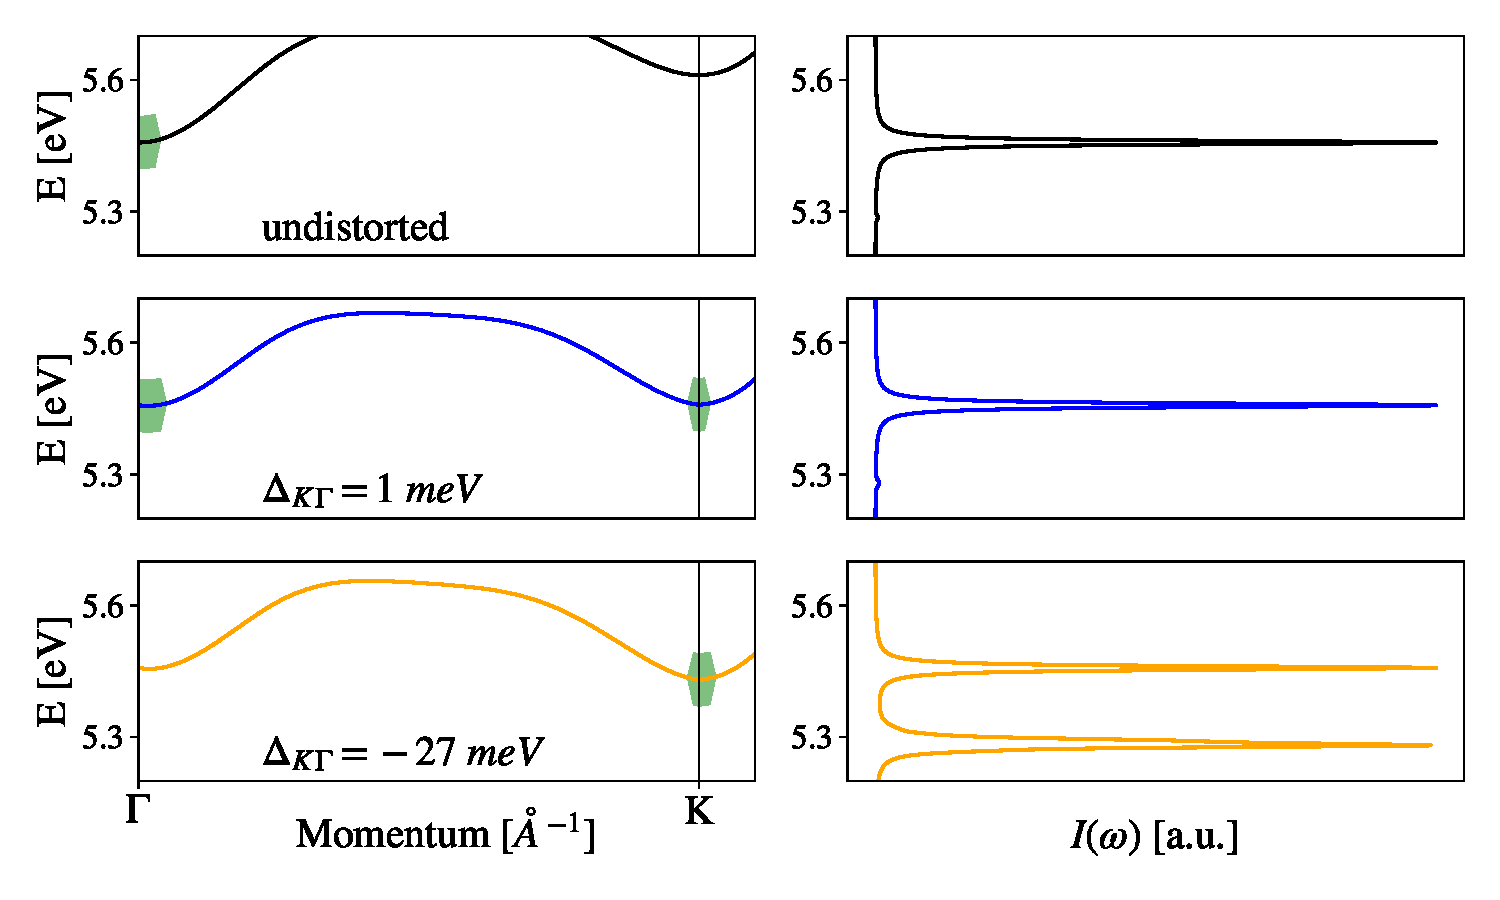
\includegraphics[width=0.8\textwidth]{mBN_distortion.pdf}
	\caption{Left column : plots of the Fourier interpolated lowest excitonic band in the dispersion of mBN, between $\Gamma$ and $K$, when momentum-dependent distortion is applied to decrease the energy at $K$. The Boltzmann occupation function is represented in green. Right column : corresponding luminescence plots, normalized to 1. The main peak is always visible and the phonon satellite gain intensity when the distortion brings the energy at $K$ lower than at $\Gamma$. \textcolor{blue}{I will put arrows or dashes to symbolize the distortion}} %MODIF : put math font for labels, think about colors; add arrow to symbolize distortion: more vspace on xlabel left to highlight Gamma and K; trim
    \label{fig:mBN_distortion}
\end{figure}
We plot the undistorted exciton dispersion and luminescence spectrum in the two upper panels of Fig. \ref{fig:mBN_distortion}. In this case the phonon-assisted satellite coming from the $K$ valley is invisible due to the energy separation. In the middle panels, we see that when $\Delta_{K\Gamma} \equiv E_1($K$) - E_1(\Gamma) = 1 meV$, the valley at $K$ gets populated, but the corresponding luminescence plots still show a phonon satellite barely visible compared to the direct peak. It is an overlap of the satellites from $\Gamma$ and from $K$, that scatter with the same phonon modes and hence have the same energy here. Finally, in the bottom panels when $\Delta_{K\Gamma} = -27$ meV, the $K$ valley is much more populated than the $\Gamma$ one and thus the phonon satellite becomes visible. 

Notice that we did not modify the exciton-phonon matrix elements unchanged for this particular plot, which is probably an inadequate approximation since the screening of the Graphite substrate screening also influences the electron-phonon coupling.\cite{sohier2021remote} It means that the change in the luminescence spectra with the distortion is only due to the change in exciton energies at finite-momentum and to the Boltzmann occupation function. As a consequence, the satellite in the bottom-right panel of Fig. \ref{fig:mBN_distortion} appears because the direct exciton is less populated. In any case, to see this effect the $K$ valley needs to be renormalized of about 170 meV, which seems unrealistic for a Graphite substrate. This is another indication to rule out the possibility that the satellite coming from $K$ could be as bright as the direct peak in the experiments.

%
\section{Preliminary results on bBN}
The Bernal form as a similar crystal structure as \acrshort{hBN}, but the stacking of the layers is AB instead of AA', with a Boron atom lying above the center of an hexagon, as illustrated in Fig. \ref{fig:hBN_stackings}.
This part of the thesis is a preliminary study for a larger work where we will also investigate the effect of different \acrshort{DFT} functionals and convergence parameters on \acrshort{bBN} properties. As a start, we used the same computational parameters as the more studied bulk \acrshort{hBN}, that can be found in Table. \ref{tab:parms} of Appendix \ref{app:comp_details_Chapt3}.

The Bernal stacking type exhibits quite a different exciton dispersion compared to hBN, as displayed in Fig. \ref{fig:bBN_excdisp}. The relative minimum along $\Gamma K$ now has an higher energy than the one at $\Gamma$. The energy of the exciton at $\Gamma$ is 5.39 eV and the minimum at $\qq=(\tfrac{1}{6},\tfrac{1}{6},0)$, which is $|\Gamma K|/2$, is 5.41 eV. This $20$ meV difference means that the indirect exciton will be populated at large effective temperatures by the Boltzmann occupation function, but only sparsely in a low-temperature measurement. We then expect most of the photoluminescence intensity coming from the direct exciton, with very little phonon-assisted satellite peaks in the spectrum.
\begin{figure}[H]
	\vspace{0.2cm}
	\setcapindent{2em}
	\centering
	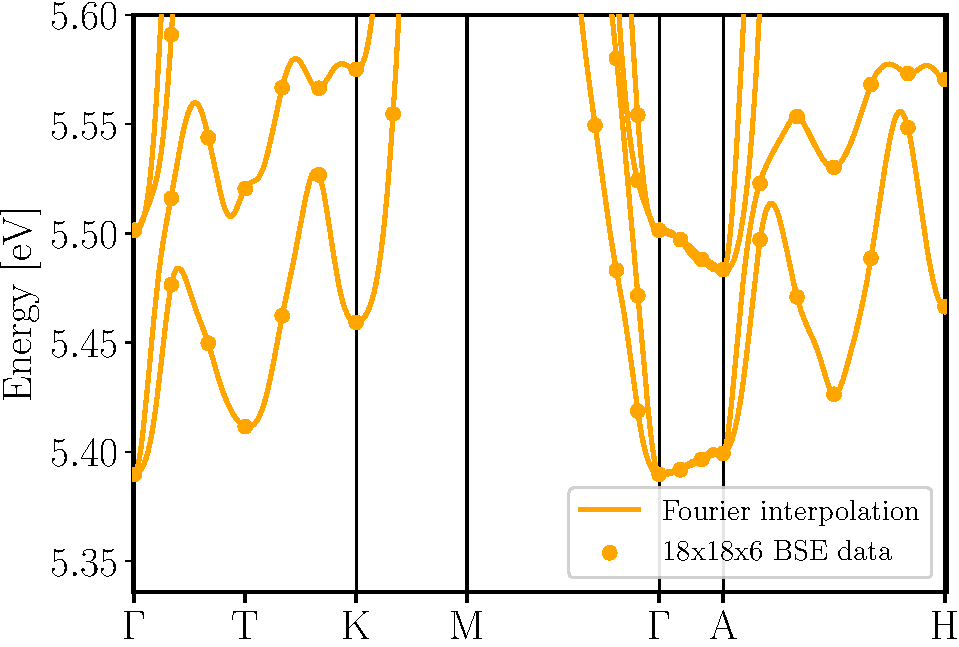
\includegraphics[width=0.8\textwidth]{bBN_excdisp.pdf}
	\caption{Calculated exciton dispersion in Bernal BN \textcolor{blue}{ticklabel is wrong it is H instead of L}} %	
    \label{fig:bBN_excdisp}
\end{figure}

We plot the exciton-phonon matrix elements for \acrshort{bBN} in Fig. \ref{fig:Gkkp_plot_hBN}. The coupling for all phonon modes is very similar than for \acrshort{hBN}, with a snowflake shape. The maximum of the coupling is around $\Gamma$ with some coupling along the $\Gamma K$ lines. Concerning the ZA and ZO modes, the matrix elements are more homogeneous with maxima at the middle of the $\Gamma K$ lines and the coupling is non-zero over the whole \acrshort{BZ}, although the magnitude is slightly lower than for hBN.
\begin{figure}[h!b]%
	\vspace{0.2cm}
	\setcapindent{2em}
	\centering
    \subfloat[All phonon modes.]{\label{Gkkp_plot_bBN:all_phonons} 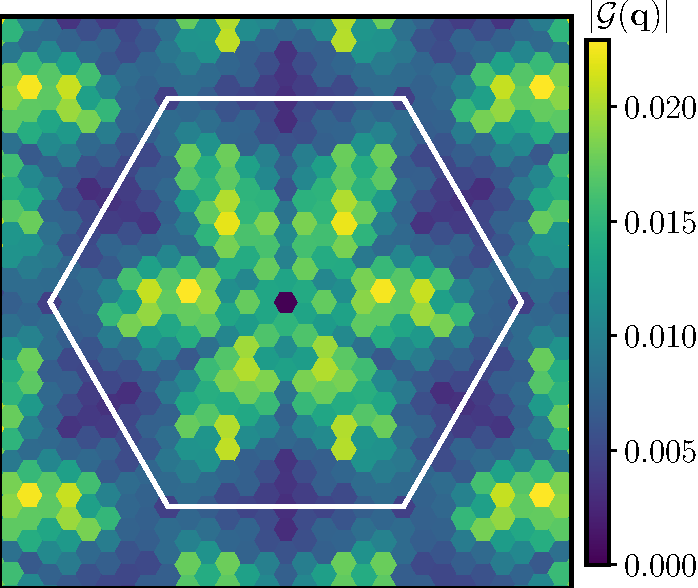
\includegraphics[width=0.45\textwidth]{bBN_Gkkp_allphonons.pdf}} \qquad 
    \subfloat[ZA+ZO modes only.]{\label{Gkkp_plot_bBN:z_only} 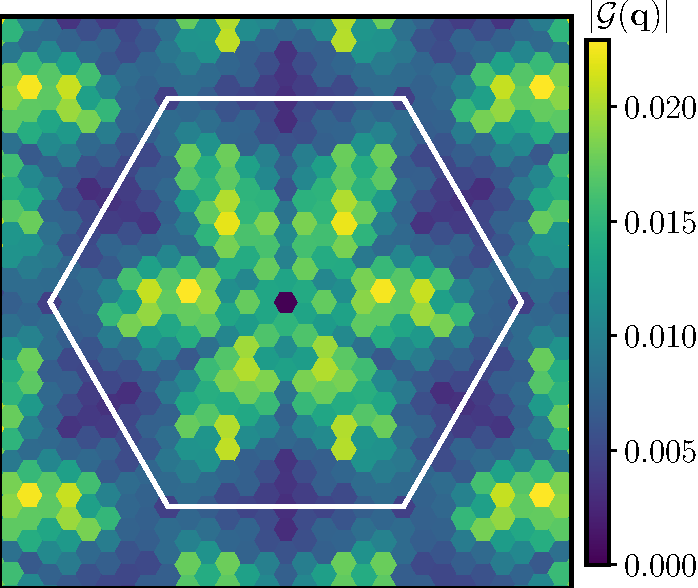
\includegraphics[width=0.45\textwidth]{bBN_Gkkp_zonly.pdf}}%
    \caption{Magnitude of the coupling between the finite-momentum excitons and the lowest-lying bright excitons in Bernal BN. Color bar is the modulus of $\mathcal{G}(\qq_\parallel)$ in eV, for a 18$\times$18 $\qq$-points grid. \textcolor{blue}{add label for colorbar}}
	\label{fig:Gkkp_plot_bBN}
\end{figure}

We found most of the contribution to the luminescence came from excitonic states at $\Gamma$ and along the $\Gamma A$ line which has a low dispersion (see Fig. \ref{fig:bBN_excdisp}). This is in agreement with the exciton-phonon matrix elements showing a higher coupling around $\Gamma$.
\begin{figure}[h!b]
	\vspace{0.2cm}
	\setcapindent{2em}
	\centering
	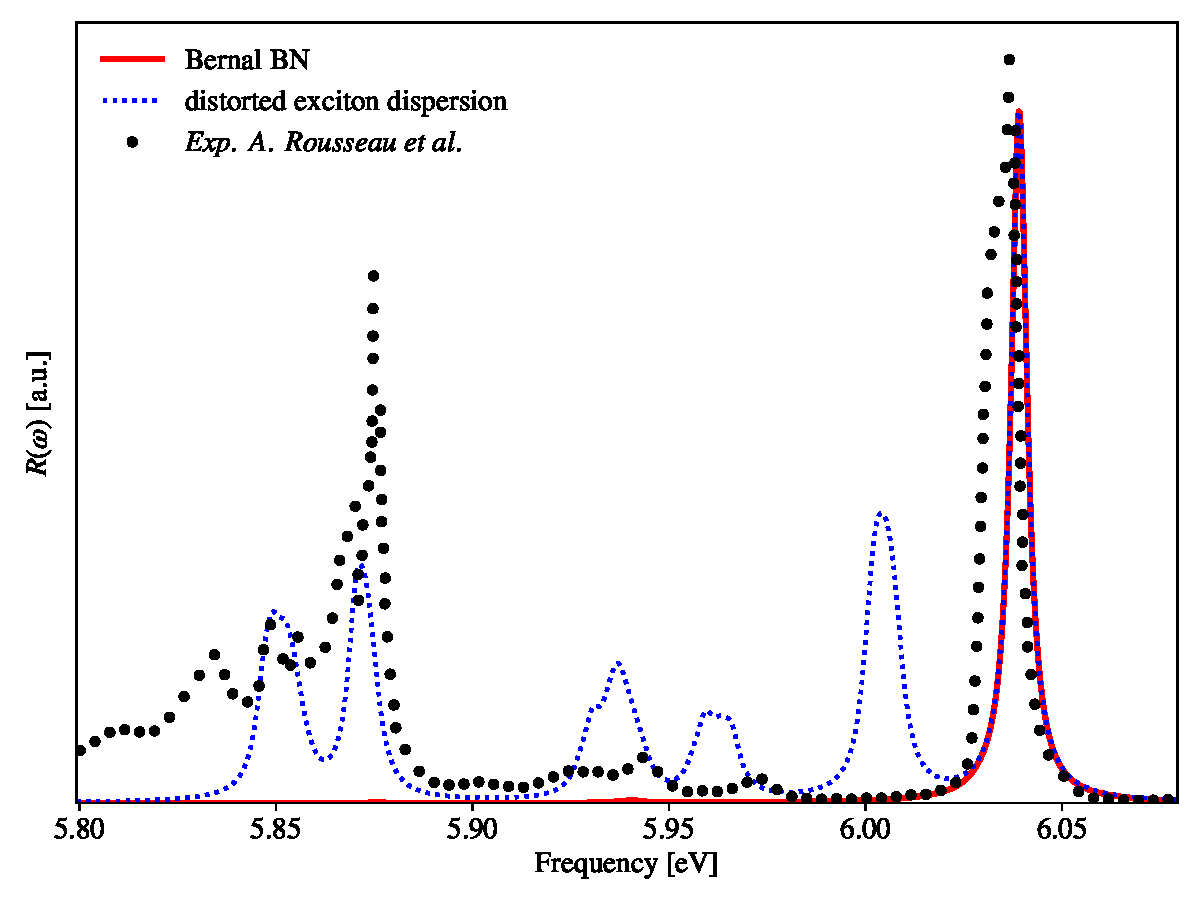
\includegraphics[width=0.8\textwidth]{bbn_pl.pdf}
	\caption{Plots of the calculated luminescence spectrum of Bernal BN, with and without exciton energy distortion, compared to experiments. We shifted the calculated spectra to match the experimental peaks.} %MODIF : align and normalize the peaks better ; add a label for T point
    \label{fig:bBN_PL}
\end{figure}

As in the \acrshort{mBN} case, we now investigate how a small distortion of the excitonic dispersion modifies the luminescence spectra. We expect that some satellite peaks will appear with intensities comparable to the direct one. In Fig. \ref{fig:bBN_PL} we report the luminescence spectra with and without distortion of the excitonic dispersion. We applied a distortion such that the valley at the middle of the $\Gamma K$ line $T = |\Gamma K|/2$ gets a few meV lower that the $\Gamma$ excitonic state : $\Delta_{\Gamma T} = -13$ meV. This corresponds to a renormalization of $\Delta E(T) = 35$ meV. \\
The luminescence plot with separated phonon contributions in Fig. \ref{fig:bBN_PL_split_phonons} allows to identify the peaks that are absent in the experiments and that are made visible with the distortion. Here we plot only the satellite contributions to luminescence. These satellites come from scattering with excitons in the new minimal $T$ valley on the $\Gamma K$ line. We see that one of the major contribution comes from a ZO phonon mode, which should be forbidden by symmetry. This is the same numerical issue that was explained above, for the ZA and ZO peaks in the spectra of \acrshort{hBN}.
\begin{figure}[h!b]
	\vspace{0.2cm}
	\setcapindent{2em}
	\centering
	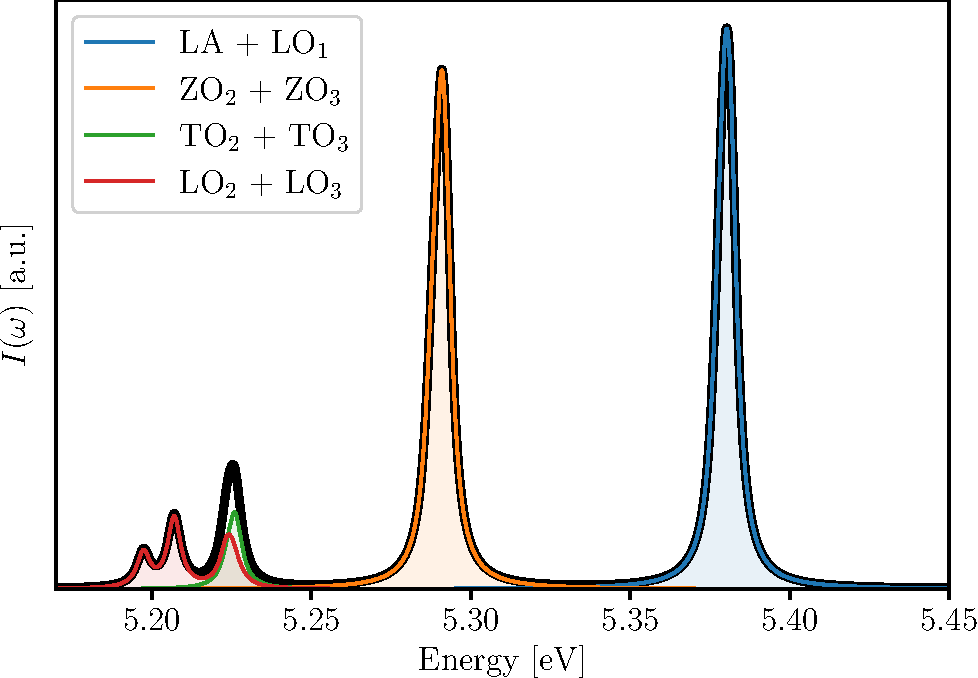
\includegraphics[width=0.8\textwidth]{bbn_pl_split_phonons.pdf}
	\caption{Plots of the satellite contributions to the luminescence spectrum of Bernal BN, where the different phonon mode contributions are separated (shifted to match the experimental peaks).} %MODIF : same modif as for hBN; shift like experiment
    \label{fig:bBN_PL_split_phonons}
\end{figure}

Since a change in the exciton energies can change drastically the luminescence spectrum, we need to perform a careful study of all the numerical parameters involved in the workflow. This is still ongoing work.


\section*{Conclusion of the chapter}

In this Chapter, we presented a first-principles methodology to calculate phonon-assisted luminescence in exciton-dominated materials. It is based on a dynamical correction to the static Bethe-Salpeter equation given by an excitonic self-energy term describing exciton-phonon interaction. Using this self-energy, we obtained a formula for the optical response that contains corrections up to first order in the exciton-phonon coupling.
Unlike previous formulations, we are also able to calculate the renormalization factor for direct transitions, which allows for a quantitative comparison between direct and phonon-assisted emission signatures.
From the optical response function, and employing a steady-state approximation, we obtained a formula for the phonon-assisted luminescence. All ingredients that enter in this formulation have been calculated \emph{ab initio}, except for the excitonic temperature relative to the occupation of excitonic states.
We first validate our approach on bulk \acrshort{hBN}, where clear and well-established experiments exist. We then applied this approach to the BN single layer, where recent discordant photoluminescence measurements were reported independently by different groups. In mBN we found that the luminescence spectrum is dominated by the single direct peak only and phonon replicas, while present, have negligible intensity. In addition, 
phonon-assisted transitions from the lowest indirect exciton remain too low in intensity to explain the measured spectra. Therefore, we rule out phonon-assisted processes as the cause of the additional spectral fine structure sometimes seen in experiment.
We support the interpretation that this fine structure is not intrinsic, nor due only to substrate effects, but depends on sample quality.

Regarding \acrshort{bBN}, our first numerical studies suggest a direct luminescence. Despite considering a small distortion of the excitonic dispersion, our spectrum still differs from the experimental one. We are investigating the role of van der Waals correction and the possible numerical problems in our procedure to provide an accurate interpretation for the experimental results.

Finally, we would like to mention that our methodology based on the dynamical self-energy has been fully implemented in the \yambo code and is applicable to other systems of interest. This formulation allows one to compute more observables than just the luminescence presented here, such as phonon-assisted absorption, exciton linewidths and relaxation rates.


	\chapter*{Conclusion}
\addcontentsline{toc}{chapter}{Conclusion}


Chap 3
perspectives
need to solve the phase problem 
natural extension to cumulant for multi phonons

Bernal : pave to way to engineering of optical properties with exciton valley positions
% 



	\appendix

	\newpage
	\printbibliography[heading=bibintoc] %% bibliographie

	\newpage
	\printendnotes						%% notes

	\setcounter{chapter}{0}
\renewcommand{\thesection}{\Alph{section}}

\chapter*{Appendices}
\newpage
\addcontentsline{toc}{chapter}{Appendices}

\numberwithin{equation}{section}
\numberwithin{figure}{section}

\section{Derivation of equations of motion for field operators}
\label{app:EOM}
Here we derive the equations of motion for the field operators in Heisenberg picture, based on \cite{martin2016interacting, stefanucci2013nonequilibrium, strinati1988application, aryasetiawan1998gw}. In the main text however, the interaction picture is used. The following derivation is left unchanged if one considers the unperturbed Hamiltonian to be the time-independent $\hat{H}$ and any other time-dependent external perturbation, which is exactly what was done in the main text.
We shall make explicit the time dependence of every term appearing in the Green's function in Eq. \eqref{eq:GF}. We start with the time evolution of the field operators. We recall some useful properties of the field operators for fermions in the Schrödinger picture :
\begin{align}
\begin{split}
	\{ \hpsi(x),\hpsidag(x')\} &= \delta (x-x') \\
	\{ \hpsi(x),\hpsi(x') \} &= \{ \hpsidag(x),\hpsidag(x') \} = 0 \\
	n(x) &= \hpsidag(x)\hpsi(x)
\end{split}	
\end{align}
 The total Hamiltonian enters the Heisenberg equation of motion for an operator $\hat{O}$:
\begin{equation}
	i\frac{d}{d t}\hat{O}_H(t) = \hat{U}^\dagger_S(t) \left[ \hat{O}(t),\hat{H} \right] \hat{U}_S(t) + \hat{U}^\dagger_S(t) (i \frac{d}{dt} \hat{O}_S(t)) \hat{U}_S(t)
\end{equation}
where the subscript $H$ and $S$ denote respectively the Heisenberg and Schrödinger pictures, and the transformation from the latter to the former is given by :
\begin{align}
\begin{split}
	\hpsi_H(x,t) &= \hat{U}^\dagger_S(t) \hpsi_S(x) \hat{U}_S(t) \\
	\hpsidag_H(x,t) &= \hat{U}^\dagger_S(t) \hpsidag_S(x) \hat{U}_S(t)
\end{split}
\end{align}
and $\hat{U}_S(t) = \exp(-i\hat{H}t) $ is the time evolution operator. In the following we drop the subscript $H$ for the field operators, as their time dependence will be explicit. The Heisenberg equation of motion for the field operator is then :
\begin{equation}
	i\frac{d}{dt} \hpsi(x,t) = \hat{U}^\dagger_S(t) \left[ \hpsi(x),\hat{H} \right] \hat{U}_S(t)
\end{equation}
and similarly for $\hpsidag$. To compute the commutator, we split the two terms of the Hamiltonian and we use the identity 
\begin{equation}
	\left[ \hpsi(x),\hat{A}\hat{B} \right] = \{ \hpsi(x),\hat{A} \}\hat{B} -  \hat{A}\{ \hpsi(x), \hat{B} \}
\end{equation}
where we take
\begin{align} 
\begin{split}
	\hat{A} &= \hpsidag(x_1) \\
	\hat{B} &= h(x_1) \hpsi(x_1)
\end{split}
\end{align}
Since $\{\hpsi(x),\hat{B}\} = 0$, then 
\begin{equation}
	\left[ \hpsi(x),\hat{H}_0\right] = h(x) \hpsi(x)
\end{equation}
Now we notice that the second term in the commutator contains 
\begin{align}
\begin{split}
	\left[ \hpsi(x), \hpsidag(x_1)\hpsidag(x_2)\hpsi(x_2)\hpsi(x_1) \right] &= \left[ \hpsi(x),\hpsidag(x_1)\hpsidag(x_2) \right] \hpsi(x_2)\hpsi(x_1) \\
	&= \left( \hpsidag(x_1) \delta(x_1-x_2) + \hpsidag(x_2)\delta(x-x_1) \right) \hpsi(x_2)\hpsi(x_1).
\end{split}
\end{align}
Therefore, 
\begin{align}
\begin{split}
	\left[ \hpsi(x),\hat{H}_{int} \right] &= \frac{1}{2} \int dx_1 \hpsidag(x_1)\hpsi(x)\hpsi(x_1) v(x,x_1) + \frac{1}{2} \int dx_2 \hpsidag(x_2)\hpsi(x_2)\hpsi(x) v(x,x_2) \\
	&= \int dx_2 v(x,x_2) \hpsidag(x_1) \hpsi(x_2) \hpsi(x)
\end{split}
\end{align}
where in the second line we used the symmetry property of the Coulomb interaction $v(x,x') = v(x',x)$.
Finally, with the compact notation $1 \equiv (\rr_1, \sigma, t_1)$, we get the equations of motion for the field operators :
\begin{align}
\begin{split}
	\frac{\partial}{\partial t_1} \hpsi(1) &= -i \left[ h(1) + \int d3 v(1,3) \hpsidag(3)\hpsi(3) \right] \hpsi(1) \\
	\frac{\partial}{\partial t_2} \hpsidag(2) &= i \left[ h(2)\hpsidag(2) + \hpsidag(2) \int d3 v(2,3) \hpsidag(3)\hpsi(3) \right]
\end{split}
\end{align}


		

\newpage
\section{From orthorombic strained cell to pseudo-hexagonal unit cell} \label{app:ortho2hex}
% \begin{figure}[!h]
%     \centering
%     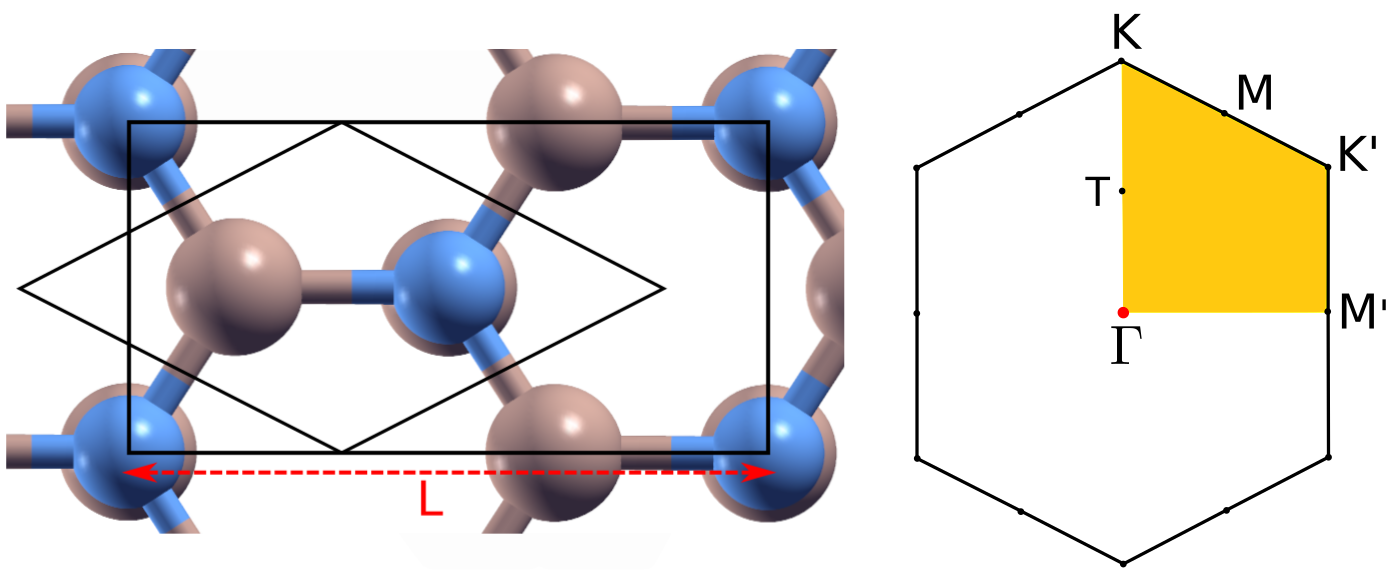
\includegraphics[width=0.5\textwidth]{AppB_structure_BZ.png}
%     \caption{This is Fig. 1 from the main text, put here for convenience.}
% \end{figure}
In our case we a have a crystal with a two-atom basis. We simulate uni-axial strain by elongating or shortening the bond length in only one cartesian direction and letting the atoms relax along the other two orthogonal directions.
It is straightforward to impose such a constraint to a lattice with orthogonal vectors, but more complicated if we had kept the equilibrium hexagonal unit cell. This is why we chose to do the relaxation of structures under strain with orthorombic cells containing 8 atoms (4 per plan).
We want to build a unit cell that preserves the symmetry and periodicity of the strained crystal, with as few atoms as possible. The following is a geometrical generalization of the transformation from orthorombic to hexagonal lattice unit cell in cartesian coordinates.\\
Take an orthorombic unit cell whose matrix in cartesian coordinates is :
\begin{equation}
\begin{pmatrix}
a & 0 & 0\\
0 & b & 0\\
0 & 0 & c
\end{pmatrix}
\end{equation}
with $a,b,c$ being arbitrary lengths.
Now we want to build a strained unit cell that resembles the equilibrium hexagonal cell the most, so that we can compare the different Brillouin zones and the paths on which we plot the electronic structure and the phonon dispersion. The rhombus representing the unit cell of the pseudo-hexagonal cell, viewed from the top, is drawn in Fig. \ref{fig:rhomb}.
\begin{figure}[b]
    \centering
    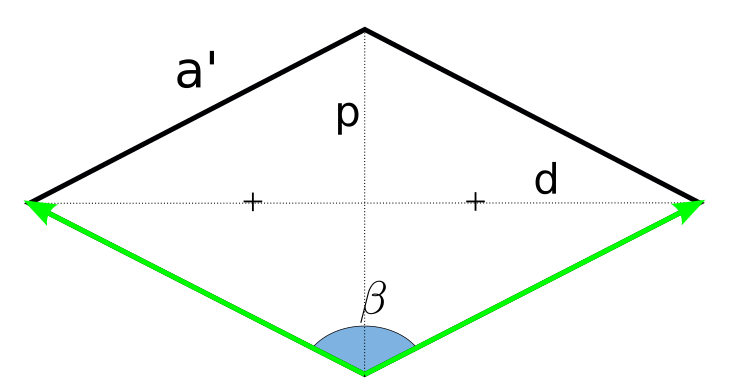
\includegraphics[width=0.5\textwidth]{AppB_rhombus.png}
    \caption{Rhombus used as the unit cell for the pseudo-hexagonal lattice with the atom positions indicated, viewed from top.}
    \label{fig:rhomb}
\end{figure}
Then we have :
\begin{align}
    a' & = \sqrt{d^2 + p^2} \\
    \beta &= \pi - 2 \tan ^{-1} \left(\frac{p}{d}\right)
\end{align}
where $d,p$ are the half diagonals of the rhombus, $a'$ is the side length and $\beta$ the angle as shown in Fig \ref{fig:rhomb}. This is a regular rhombus in the sense that all sides have equal length and the diagonals are orthogonal. The length of the diagonals is obtained from the knowledge of the orthorombic cell, as shown in Fig. \ref{fig:strain_BZ} in the main text.
Then the matrix of this rhombus unit cell, expressed in cartesian coordinates, is :
\begin{equation}
\begin{pmatrix}
a' & 0 & 0\\
a'\cos\beta & a'\sin\beta & 0\\
0 & 0 & c
\end{pmatrix}
\end{equation}
The first two lines are the vectors in green in Fig. \ref{fig:rhomb}. The third vector $c$ is the one perpendicular to the atomic planes and is the same than the orthorombic $c$.
In the equilibrium case, we have $\beta = 120$\textdegree, then this matrix reduces to :
\begin{equation}
\begin{pmatrix}
a' & 0 & 0\\
-a'/2 & a'\sqrt{3}/2 & 0\\
0 & 0 & c
\end{pmatrix}
\end{equation}
which is the standard hexagonal-lattice unit cell. We now have built a 2-atom unit cell which we used to compute electronic, phononic and optical properties of our strained materials. We checked that both the orthorombic and the pseudo-hexagonal unit cells form the same strained crystal when periodically repeated in all directions.
			%% annexes

\end{document}
